\documentclass[a4paper, 12pt]{report}
\usepackage[total={17cm,25cm}, top=2.5cm, left=2.5cm, right=2.5cm,  includefoot]{geometry}
\usepackage[utf8]{inputenc}
\usepackage{array}
\usepackage{multirow}
\usepackage{hhline}
\usepackage{gensymb}
\usepackage{graphicx}
\graphicspath{ {} }
\usepackage[czech]{babel}
\usepackage{enumitem}
\usepackage{pdfpages}
\usepackage{amsmath}
\usepackage{verbatim}
\usepackage{listings}
\usepackage{hyperref}
\usepackage{amssymb}
\usepackage{graphicx} %graphics files inclusion
\usepackage{amsmath} %advanced maths
\usepackage{amssymb} %additional math symbols
\usepackage{rotating}


\usepackage[utf8]{inputenc} % LaTeX source encoded as UTF-8

\usepackage{graphicx} %graphics files inclusion
\usepackage{amsmath} %advanced maths
\usepackage{amssymb} %additional math symbols
\usepackage{rotating}
\usepackage{pdfpages}

\usepackage{dirtree} %directory tree visualisation
% % list of acronyms
% \usepackage[acronym,nonumberlist,toc,numberedsection=autolabel]{glossaries}
% \iflanguage{czech}{\renewcommand*{\acronymname}{Seznam pou{\v z}it{\' y}ch zkratek}}{}
% \makeglossaries


\usepackage{etoolbox}
\patchcmd\thebibliography{\sloppy}{\tolerance 500\relax
                                   \emergencystretch 1em\relax }{}{\fail}
 

\newcommand{\tg}{\mathop{\mathrm{tg}}} %cesky tangens
\newcommand{\cotg}{\mathop{\mathrm{cotg}}} %cesky cotangens


\pagestyle{empty} % vypne číslování stránek




\usepackage[OT2,OT1]{fontenc}
\newcommand\cyr
{
\renewcommand\rmdefault{wncyr}
\renewcommand\sfdefault{wncyss}
\renewcommand\encodingdefault{OT2}
\normalfont
\selectfont
}
\DeclareTextFontCommand{\textcyr}{\cyr}
\def\cprime{\char"7E }
\def\cdprime{\char"7F }
\def\eoborotnoye{\char’013}
\def\Eoborotnoye{\char’003}


\usepackage{graphicx}
\graphicspath{ {figures/} }
\usepackage{array}

\begin{document}



\begin{titlepage}
\begin{center}
\noindent
\Large {\textbf{České vysoké učení technické v Praze}\\Fakulta stavební}
\vspace{3cm}

\huge

%vložení loga cvut
\begin{figure}[h!]
	\centering
	
\includegraphics[width=7cm]{logo.png}
\end{figure}

\vspace{0.5cm}

\Huge  
\textbf{Diplomová práce}\\
\Large Využití virtuální reality při dokumentaci a vizualizaci památkových objektů
\end{center}

\vfill

\begin{flushleft}
\normalsize \textbf{Autor:}
\normalsize Bc. Robin Pflug \\
\normalsize \textbf{Vedoucí práce:}
\normalsize Prof. Dr. Ing. Karel Pavelka\\
\normalsize \textbf{Katedra:} geomatiky\\
\normalsize \textbf{Akademický rok:} 2019/2020
\end{flushleft}

\end{titlepage}

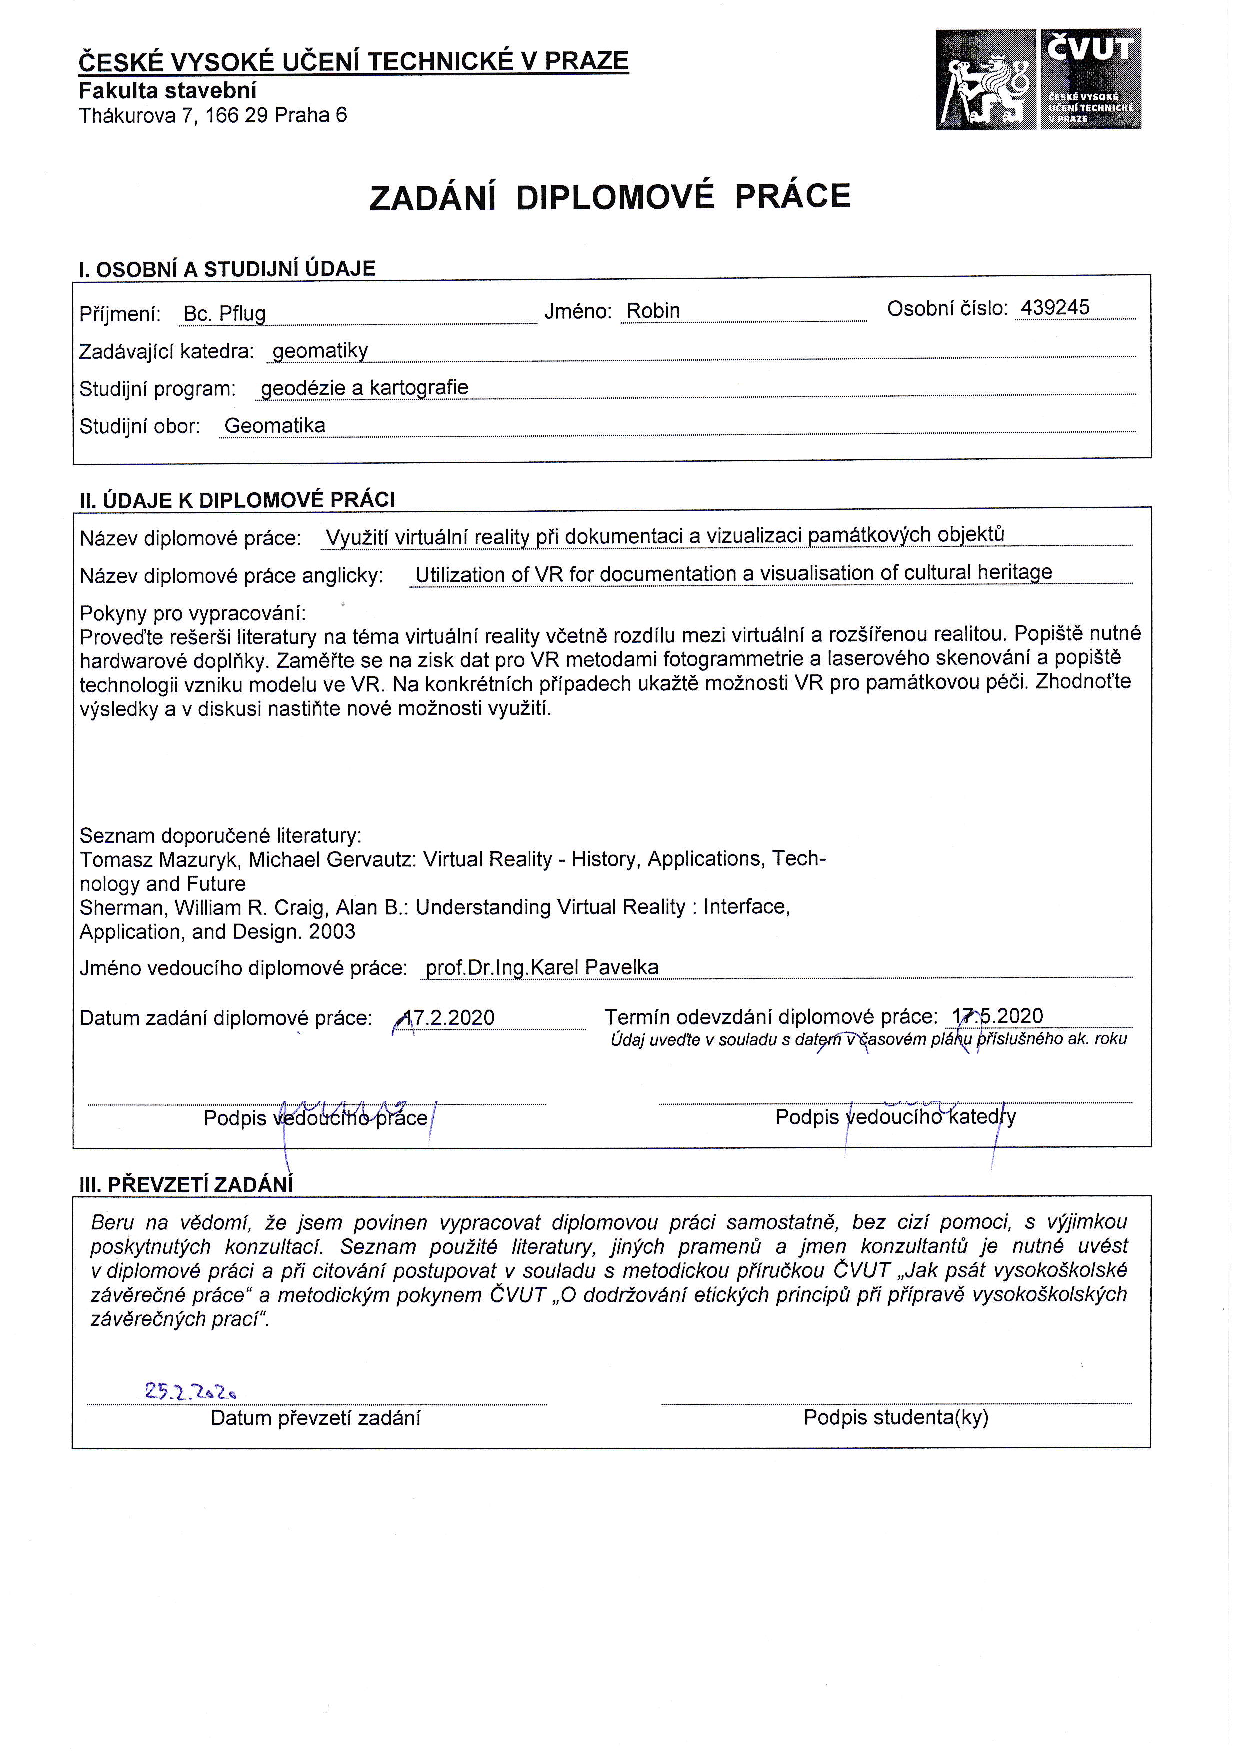
\includepdf[page=-]{zadani.pdf}

\newpage


\renewcommand{\abstractname}{}
\begin{abstract}
\vfill
\begin{large}
\textbf{Poděkování}
\end{large}\\
\\
Děkuji Prof. Dr. Ing. Karlu Pavelkovi za odborné vedení práce a cenné rady. Velké díky také patří Ing. Karlu Pavelkovi za mnoho rad a typů týkajících se nejen virtuální reality, ale také tvorby a zpracování modelů historických objektů. V neposlední řadě děkuji své rodině a přátelům za silnou podporu během celého studia. 
\end{abstract}

\renewcommand{\abstractname}{}
\begin{abstract}
\vfill
\begin{large}
\textbf{Prohlášení}
\end{large}\\
\\
Prohlašuji, že jsem předloženou práci vypracoval(a) samostatně a že jsem
uvedl(a) veškeré použité informační zdroje v souladu s Metodickým pokynem
o etické přípravě vysokoškols-\\kých závěrečných prací.\\
	Beru na vědomí, že se na moji práci vztahují práva a povinnosti vyplývající ze zákona č. 121/2000 Sb., autorského zákona, ve znění pozdějších předpisů, zejména skutečnost, že České vysoké učení technické v Praze má právo na uzavření licenční smlouvy o užití této práce jako školního díla podle § 60 odst. 1 autorského zákona.\\
\\
\\
\\ 
\\
V Praze dne 24. května 2020	 \hfill .................................
\end{abstract}

\renewcommand{\abstractname}{}
\begin{abstract}
\vfill
České vysoké učení technické v Praze\\
Fakulta stavební\\
\copyright 2020 Robin Pflug. Všechna práva vyhrazena.\\
\textit{Tato práce vznikla jako školní dílo na Českém vysokém učení technickém v Praze, Fakultě stavební. Práce je chráněna právními předpisy a mezinárodními úmluvami o právu autorském a právech souvisejících s právem autorským. K jejímu užití, s výjimkou bezúplatných zákonných licencí, je nezbytný souhlas autora.}\\
\\
\textbf{Odkaz na tuto práci}\\
\\
Pflug, Robin. \textit{Využití virtuální reality při dokumentaci a vizualizaci památkových objektů}. Diplomová práce. \\
Praha: České vysoké učení technické v Praze, Fakulta stavební, 2020.

\end{abstract}

\renewcommand{\abstractname}{}
\begin{abstract}
\begin{large}
\textbf{Abstrakt}
\end{large}\\
\\
Cílem této práce je ukázat možnosti využití VR pro památkovou péči. Podstatou práce je tvorba a zpracování modelů historických objektů pro následnou vizualizaci ve VR. Data ve formě fotografií byla získána běžně dostupnými kompaktními fotoaparáty. Pro tvorbu modelů byla použita IBMR technologie. Součástí práce byla také tvorba virtuálního prostředí, do kterého byly následně umisťovány dokumentované objekty. Pro virtuální modely byly, za účelem vhodné vizualizace, vytvářeny nové materiály, které vznikly z příslušných textur a normálových map. Výsledná vizualizace obsahuje krajinu, budovu virtuálního muzea a modely historických objektů. Výsledky práce jsou prezentovány formou VR.
\vfill
\textbf{\\Klíčová slova:} virtuální realita, rozšířená realita, laserové skenování, IBMR, vizualizace,\\ 
fotogrammetrie, Unreal engine, SketchUp, Agisoft Metashape, textury, památková péče
\end{abstract}

\renewcommand{\abstractname}{}
\begin{abstract}
\begin{large}
\textbf{Abstract}
\end{large}\\
\\
Aim of this diploma thesis is to show the possibilities of using VR for monument care. The creation and processing of historic objects models for subsequent visualization in VR is the essence of the work. Photographs, as data for this work, were obtained by commonly available compact cameras. The models were created by using IBMR technology. Part of the work is the creation of a virtual environment, where the documented objects are placed subsequently. For suitable visualization were created new materials for the virtual models, which arise from the relevant textures and normal maps. The visualization result includes a landscape, a virtual museum building, and models of historic buildings. The result of the work is presented in the form of VR.
\vfill
\textbf{\\Keywords:} virtual reality, augmented reality, laser scanning, IBMR, visualization, \\
photogrammetry, Unreal engine, SketchUp, Agisoft Metashape, textures, monument care
\end{abstract}

\pagestyle{plain}     % zapne obyčejné číslování
\setcounter{page}{1}  % nastaví čítač stránek znovu od jedné
\tableofcontents
\thispagestyle{plain}

\chapter*{Seznam zkratek}
\textbf{HMD} Head-Mounted Display\\
\textbf{VR} Virtual Reality (Virtuální realita)\\
\textbf{AR} Augmented Reality (Roršířená realita)\\
\textbf{DOF} Degree Of Freedom\\
\textbf{IR} InfraRed\\
\textbf{LED} Light-Emitting Diode\\
\textbf{SLAM} Simultaneous Localization and Mapping (Souběžná lokalizace a mapování)\\
\textbf{FOV} Field Of View\\
\textbf{OS} Operating Systém (Operační systém)\\
\textbf{CPU} Central Processing Unit\\
\textbf{RAM} Random-Access Memory\\
\textbf{GPU} Graphics Processing Unit\\
\textbf{OLED} Organic Light Emitting Diode\\
\textbf{PS4} PlayStation 4\\
\textbf{IBMR} Image-Based Modeling and Rendering\\
\textbf{RPAS} Remotely Piloted Aircraft Systems\\
\textbf{UE4} Unreal Engine 4\\
\textbf{HTC} High Tech Computer (Corporation)\\
\textbf{N-RoSy} N-way rotational symmetry\\
\textbf{MB} MegaByte\\
\textbf{IMU} Inertial Measurement Unit\\
\textbf{MEMS} MicroElectroMechanical Systems\\
\textbf{TOF} Time Of Flight\\

\listoffigures

\newpage

\chapter{Úvod}
Virtuální realita (VR) je pojem, se kterým se v dnešní době setkal snad každý člověk, jenž se alespoň okrajově zajímá o svět moderních technologií. Virtuální realita se pomalu stává nedílnou součástí moderního světa, ať už se jedná o oblast počítačových her, vědeckých prací, lékařství, vojenství, strojírenství či speciální formy výuky.\\
Snaha zachytit co nejvěrněji okolní realitu je stará jako lidstvo samo. Již primitivní lidé svými malbami v jeskyních tvořili jistou formu umělé reality vzdáleně se přibližující k virtuální realitě v dnešním slova smyslu. Zdánlivě nesouvisející jeskynní malby s tématem této práce však mají hlubší význam. Mají význam ve smyslu snahy člověka vyvíjet metody pro tvorbu a prezentaci nejrůznějších objektů, které nemusí být ani skutečné, co nejvěrnější formou.[1] V dnešní době nejčastěji rozumíme pod pojmem virtuální realita soubor počítačového softwaru a hardwaru, který nám dokáže potlačit vjemy reálného světa a navodit vjemy světa uměle vytvořeného. Možnosti výběru a formy virtuální reality jsou v současné době značně obsáhlé a budou také předmětem následujících kapitol.\\
Tématem diplomové práce je využití virtuální reality při dokumentaci a vizualizaci \\památkových objektů. Hlavním cílem je vytvoření virtuálního muzea, které bude obsahovat vybrané historické objekty zdokumentované metodami fotogrammetrie a zpracované pro vhodnou prezentaci formou VR. Budova virtuálního muzea i okolní prostředí bylo vytvořeno uměle za pomoci grafických počítačových softwarů. Veškeré výsledné objekty jsou prezentovány ve formě virtuální reality. Přínosem diplomové práce je ukázka možností novodobé dokumentace i prezentace historických objektů, v takové formě, u které není možné předměty jakkoliv poškodit či zničit, a dále je možno je analyzovat, aniž bychom s nimi museli být v kontaktu.\\
\\
Dokumentovány byly celkem 4 objekty různých velikostí. Jednalo se o dva římské sarkofágy, sochu sv. Petra a malou chrámovou stavbu z hinduistické svatyně. Objekty byly fotografovány běžně dostupnými kompaktními fotoaparáty a následně zpracovány moderní IBMR technologií do modelů o vysokém rozlišení včetně textur. Pro potřeby vhodné vizualizace ve VR byla poté provedena retopologie objektů a tvorba normálových map textur. Takto připravené modely byly umístěny do předem vytvořeného prostředí ve VR. Na závěr byly vytvořeny nové materiály modelů složené z textur o vysokém rozlišení a příslušných normálových map.\\
\\
První část práce obsahuje rešerši literatury zaměřenou na témata týkající se VR, AR, metod sledování pohybu používané pro VR i AR zařízení a metod fotogrammetrie a laserového skenování pro sběr dat. Část druhá je zaměřená na VR, konkrétně na její definici, historii, využívané metody sledování pohybu zařízení, současný hardware a využití v různých oborech. Poslední kapitola teoretické části této práce je věnována IBMR technologii. V kapitole je popsán způsob sběru dat i tvorba mračen bodů touto technologií. Popis praktické části této práce je rozčleněn do čtyř kapitol. Kapitola \textit{Tvorba virtuálního muzea} popisuje způsob a postupy, jakými vznikalo veškeré virtuální prostředí pro vizualizaci historických objektů ve VR. Další kapitoly jsou pak věnovány historickým objektům: popisu způsobu dokumentace a zpracování do virtuálních modelů včetně následné vizualizace ve VR. Obsahem závěru je zhodnocení výsledků zpracování a vizualizace dat a nastínění nových možností využití VR pro památkovou péči.\\
\\
Textová část práce byla vytvořena ve volně dostupném softwaru LaTeX, na základě šablony poskytované Českým vysokým učením technickým v Praze. LaTeX obsahuje prvky k výrobě kvalitní technické i vědecké dokumentace, podle samotných autorů softwaru se jedná o standart pro zveřejňování vědeckých dokumentů.[3]

\chapter{Rešerše literatury}
Tato práce se zaměřuje na dvě hlavní témata: \\
1) Tvorba a prezentace modelů v prostředí VR, včetně konkrétních ukázek možností využití VR pro památkovou péči v podobě případových studií. \\
2) Možnosti sběru dat moderními metodami fotogrammetrie a laserovým skenováním.\\
\\
Následující rešerše se zaobírá významnými pracemi z oblasti VR, ale je zaměřena i na možnosti rozšířené reality (AR). Technologie virtuální i rozšířené reality zaznamenává v současnosti výrazný rozvoj v mnoha oblastech využití. Tento rozvoj je ovšem způsoben uvedením dostupných zařízení pro veřejnost na trh v období let 2010 až 2012. V předchozích vývojových etapách byla většina VR technologií pro veřejnost nedostupná nebo nedosahovala potřebných kvalit pro potřeby odborného využití. Vzhledem k tomu, že se jedná o obor rozvíjející se především v 21. století, vychází tato práce především z internetových zdrojů zabývajících se problematikou VR i AR. 

\section{VR}
Dílo \textit{Understanding Virtual Reality : Interface, Application, and Design} vytvořené dvojicí autorů William R. Sherman a Alan B. Craig podrobně rozebírá definici a jednotlivé prvky VR. Podle autorů není definice VR jednotná, ovšem v klíčových oblastech se většina definic shoduje. VR definují čtyři klíčové prvky: virtuální svět, ponoření, smyslová zpětná vazba a míra interaktivity. Nezbytnou součástí každé VR je vhodná kombinace těchto hlavních elementů. Části díla podrobně popisující co tvoří VR jsou na závěr shrnuty do pěti vět. VR je komunikační médium. VR vyžaduje fyzické ponoření. VR stimuluje smysly. VR je interaktivní. VR může psychicky pohltit uživatele. [1]\\
\\
Pro ucelený přehled o historii, současnosti i budoucnosti VR posloužilo dílo \textit{Virtual Reality - History, Applications, Technology and Future} od autorů Tomasz Mazuryk a Michael Gervautz. Historie VR je zde mapována od 60. let 20. století. Jako první popisuje VR Ivan Sutherland v roce 1965. Od této doby zaznamenala VR značný rozvoj ve všech směrech: hardware, software, dostupnost. T. Mazuryk a M. Gervautz uvádí ve svém díle několik nejdůležitějších milníků ve vývoji VR. Autoři také popisují co je a co není považováno za VR, základní prvky i vlastnosti VR a moderní způsoby využití. Rozsáhlá část díla také mapuje možnosti hardwaru a podrobně rozebírá způsoby tvorby virtuálního světa. [5]\\
\\
Dílo \textit{Virtual Reality} od autora Steven M. LaValle podrobně popisuje a vysvětluje prvky a principy používané pro tvorbu VR. Autor nejprve v úvodu definuje pojem VR, dále se pak zabývá vhodným hardwarem i softwarem pro prezentaci VR. Podrobně je v díle popisována i fyziologie lidského vidění a od ní odvozené požadavky na kvalitu zařízení. V druhé polovině knihy je popsána fyzika virtuálního světa, metody sledování pohybu VR zařízení, možnosti interakce ve virtuálním prostředí a na závěr autor uvádí možné způsoby hodnocení zařízení pro VR. [49]\\
\\
Některé informace, týkajících se VR, byly čerpány také z internetového informačního portálu \textit{Virtual Reality Society} dostupného na www.vrs.org.uk. [4]\\
\\
Studie Vladimíra Jůvy: \textit{Virtuální muzeum a nové možnosti
vzdělávání} je zaměřena na moderní muzejnictví, způsoby digitalizace muzeí a také na jejich edukační význam. Autor nejprve popisuje vzdělávací význam moderního muzea, dále se pak zabývá vhodnou digitalizací kulturního dědictví a možnostmi virtuálního muzea. Virtuální muzea jsou ze své podstaty závislá na kvalitě zpracování VR. Poslední část studie je věnována propojení prvků vzdělávání s virtuálním muzeem. [35]\\
\\
Vzdělávací portál VIRTUALSPEECH byl využit jako rozšiřující zdroj informací o jednotlivých historických etapách vývoje VR ve světě. Portál obsahuje informace o objevech, publikacích i vývoji hardwaru, které výrazně ovlivnily vývoj moderní VR. Historie je mapována od roku 1838, ve kterém Sir Charles Wheatstone popsal binokulární vidění. [6] Jako pohled do historické představy o budoucnosti VR bylo vhodným zdrojem dílo \textit{The Ultimate Display} od Ivana E. Sutherlanda. [8] \\
\\
Publikací, zabývajících se hardwarem pro VR, je v digitální podobě na internetu mnoho. V důsledku rychlého rozvoje této technologie v posledních několika letech neexistují téměř žádná tištěná díla s danou aktuální tématikou. Dílo \textit{Designing for VR: Beginners Guide for ID and IxD} od Nth Screen shrnuje současný trh s VR a popisuje jednotlivé elementy hardwaru několika předních výrobců. [18] Informační server The Verge poskytuje podrobný rozbor dílů zařízení pro VR od mnoha výrobců včetně přídavného hardwaru. [19] Podrobné informace o parametrech i složení hardwarů jsou dostupné z internetových portálů \textit{PCMag} na www.pcmag.com [25] a \textit{Tom's Hardware} dostupné z www.tomshardware.com. [26]\\
\\
Doplňující informace ke konkrétním zařízením byly čerpány přímo z internetových stránek výrobců: pro HTC VIVE dostupné z www.vive.com [20], Oculus dostupné z \\www.oculus.com [23], PlayStation dostupné z www.playstation.com [24] a pro zařízení od společnosti Valve Index dostupné z www.valvesoftware.com [27].\\
\\
Využití VR nalezneme v mnoha oborech. Publikace, informace a díla týkající se možností jak využít virtuální svět v jednotlivých oborech, jsou snadno dostupné v elektronické i tištěné podobě. Dílo s názvem \textit{Virtual Reality \& Augmented Reality in Industry} od autorů Dengzhe Ma, Jurgen Gausemeier, Xiumin Fan a Michael Grafe se zabývá využitím VR v mnoha průmyslových odvětvích a bylo cenným zdrojem informací i pro tuto práci. [31] Způsoby využití VR v oblasti lékařství jsou popsány na portálu \textit{docwire} provozovaného společností DocWire News, dostupného z www.docwirenews.com [33]. Publikace \textit{Virtual Museum Exhibitions} popisuje možnosti a tvorbu virtuálních muzeí včetně vnitřního fungování. [34]\\
\\
Studie \textit{Augmented and Virtual Reality Evolution and Future Tendency} od autorů Luis Muñoz-Saavedra, Lourdes Miró-Amarante a Manuel Domínguez-Morales je zaměřena na vývoj nových technologií v oblasti AR i VR, včetně nastínění budoucích trendů. První část textu je zaměřena na analýzu vývoje publikací i her zaměřených na AR a VR v posledních letech. Výsledky ukazují klesající tendenci v počtu nově vznikajících odborných publikací oproti letům předchozím. Analýza nově vznikajících her disponující možností použití VR vykazuje obdobnou klesající tendenci. Autoři uvádí, že nižší popularita je pravděpodobně zapříčiněna rozšířením technologií mezi širokou veřejnost, více než v oblasti výzkumu. Studie se také zabývá rozložením četnosti publikací na dané téma v jednotlivých světových regionech. Výsledky uvádí, že většina publikací na téma VR nebo AR je v oblastech výzkumu, zdravotnictví, vzdělávání a průmyslu. Autoři v závěru studie uvádí, že výzkum v oblasti VR i AR bude pokračovat, ale počty publikací budou klesat dokud nedosáhnou stabilní hodnoty. [48]

\begin{figure}[h!]
	\centering
	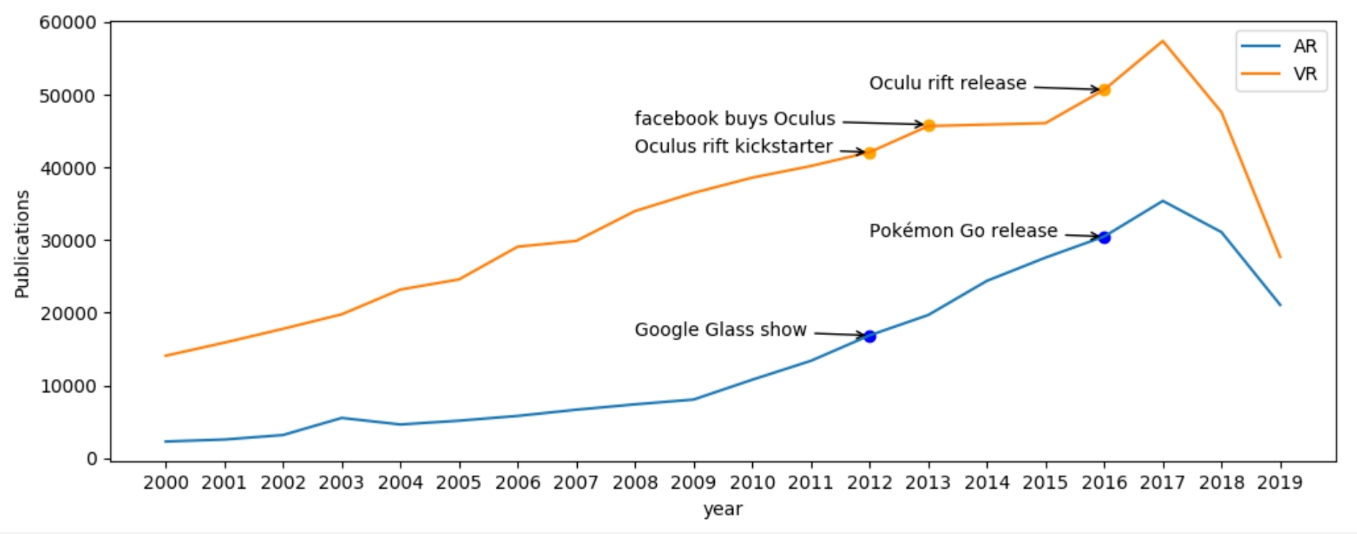
\includegraphics[width=16cm]{publikace_VR.jpg}
	\caption{Vývoj počtu nově vzniklých publikací v oblasti AR a VR. [48]}
\end{figure}

\section{AR}
Autor knihy, \textit{Handbook of Augmented Reality}, Borko Furht definuje rozšířenou realitu jako přímý nebo nepřímý pohled na reálné prostředí v reálném čase, který je rozšířen o počítačem generované informace. Jinými slovy, rozšířená realita propojuje reálný svět s virtuálním. Rozdíl AR od VR je především v míře ponoření. Ve VR je uživatel zcela ponořen, aniž by viděl skutečný svět. AR uživateli pouze rozšiřuje skutečný svět prostřed-nictvím virtuálních objektů. Rozšířená realita nemusí vytvářet výlučně zrakové vjemy, ale také vjemy působící na ostatní smysly. Autor v knize popisuje historii AR, která je úzce spjata s historií VR. Oproti VR se AR dostává mezi širokou veřejnost již na přelomu století, to bylo zapříčiněno prudkým rozvojem mobilních zařízení, které AR zprostředkovávaly.\\
Rozsáhlé dílo poskytuje kvalitní informace o současných i budoucích trendech AR, popisuje základy, principy i systémy rozšířené reality. Značná část je věnována také způsobům využití AR. [52]\\
\\
Publikace \textit{Augmented reality technologies, systems and applications} od autorů Julie Carmigniani, Borko Furht, Marco Anisetti, Paolo Ceravolo, Ernesto Damiani a Misa Ivkovic zkoumá současný stav techniky, systémů a aplikací v oblasti AR. Autoři popisují práce prováděné mnoha různými výzkumnými skupinami, různé účely AR systémů a problémy, které vznikají při vytváření některých AR aplikací. Autoři také spekulují o budoucím vývoji AR. Obsahem díla je opět rozlišení a popis rozdílu mezi VR a AR. AR je zde rozsáhle specifikována. V publikaci je opět vyzdviženo, že AR může potenciálně působit na různé smysly. AR lze také použít k rozšíření nebo nahrazení chybějících smyslů uživatele smyslovou substitucí, jako je například simulace zraku nevidomých uživatelů prostřednictvím zvukových podnětů, nebo rozšíření sluchu pro neslyšící uživatele pomocí vizuálních podnětů. Dílo bylo zdrojem informací pro pochopení metod počítačového vidění v AR. [53]\\
\\
Studie \textit{Effects of Virtual Reality and Augmented
Reality on Visitor Experiences in Museum} od autorů Timothy Jung, M. Claudia tom Dieck, Hyunae Lee, and Namho Chung se zabývá dopadem zařazení VR a AR do kontextu muzeí. Studie například uvádí, že narozdíl od VR, AR poskytuje návštěvníkům muzea přirozený reálný zážitek, který je pouze částečně rozšířen o digitální obsah. U VR i AR je zde objasňován význam osobní, sociální a enviromentální přítomnosti uživatele. Studie se zabývá také rostoucí významností AR i VR v oblasti turismu. Velký potenciál je přikládán také edukačnímu efektu AR a VR. Studie ukázala, že VR i AR výrazně zlepšují hodnotu zážitku návštěvníka muzea.[54]

\section{Metody sledování pohybu}
Metody sledování pohybu HMD i rukou uživatele jsou nedílnou součástí profesionálních VR zařízení. \\
\\
Článek od autorů Miguela Riba, Axele Pinza a Antona L. Fuhrmanna, \textit{A new Optical Tracking System for Virtual and Augmented Reality Applications}, popisuje vlastnosti a parametry, které musí splňovat kvalitní zařízení disponující sledováním pohybu v oblasti VR i AR. Autoři v druhé části popisují vlastní metodu sledování pohybu založenou na stereo vizi sledovacího zařízení, která je vhodná pro VR i AR.[38]\\
\\
Publikace \textit{Head Tracking for the Oculus Rift}, ve které autoři Steven M. LaValle, Anna Yershova, Max Katsev a Michael Antonov představují metody využívané pro přesné sledování pozice zařízení Oculus Rift, detailně popisuje a vysvětluje způsob výpočtu a oprav polohy sledovaného zařízení v reálném čase. Autoři podrobně popisují problematiku a způsoby korekcí tzv. driftu a náklonu, včetně vzorových vzorců a grafů, prostřednictvím gyroskopu a akcelerometru. Druhá část textu je věnována třem metodám, které poskytují snížení hodnoty latence zařízení využitím predikce pohybu. [39]\\
\\
Historické metody sledování pohybu rukou, které využívala zařízení pro VR, jsou kvalitně popsány na informačním portále \textit{Jeremy Norman's: HistoryofInformation.com}. Článek popisuje vznik a vývoj amerického patentu, jehož autorem byl Thomas G. Zimmerman, který spočíval v optickém ohybovém senzoru umístěným v rukavici. Tímto zařízením bylo možné sledovat ohyb prstů uživatele. Následný rozvoj technologie umožnil vytvoření prvních rukavic se sledováním pohybu. První komerčně dostupné rukavice se sledováním pohybu použila firma Nintendo. [9]\\
\\
Informační server Upload dostupný z uploadvr.com posloužil jako obsáhlý zdroj informací o současných metodách sledování pohybu, které jsou využívány v oblasti moderních VR zařízení (Oculus, PlayStation VR, HTC Vive). Článek informuje o rozdílu mezi metodou sledování pohybu s třemi a šesti stupni volnosti. Druhá část textu je věnována metodám a možnostem sledován pohybu právě s šesti stupni volnosti. [16]\\
\\
Do oblasti VR a AR lze vložit i metody SLAM, které umožňují lokalizaci pohybujícího se zařízení. Diplomová práce Bc. Jana Najmana s názvem \textit{Aplikace SLAM algoritmů pro vozidlo s čtyřmi řízenými koly} odborně vysvětluje SLAM algoritmy. [21]\\
\\
Doplňující informace o používaných metodách pro sledování pohybu u jednotlivých zaříze-ních byly čerpány také z internetové stránky \textit{androidcentral} dostupné z www.androidcentr-al.com. [22]

\section{Metody sběru dat}
Využití metod fotogrammetrie a laserového skenování ke sběru dat pro trojrozměrné modely je v současnosti populární téma. Přímo na ČVUT vzniklo několik publikací zabývající se touto problematikou. Informačně přínosné dílo je \textit{Exaktní metody průzkumu památek s využitím geodetických a geofyzikálních metod}, které vytvořil Karel Pavelka a kolektiv. Práce popisuje moderní metody, které jsou vhodné k dokumentaci v oblasti památkové péče a porovnává je s výsledky metod starších. První část díla je věnována fotogrammetrii a metodám s ní spjatých. Veškeré popsané metody jsou zde doplněny o reálné příkladové výsledky. Obsahem této části je také metoda IBMR, která je využita v této práci. Druhá kapitola knihy provádí metodami, využitím a výsledky 3D skenování. Další informačně podstatnou kapitolou je Dokumentace soch a stavebních prvků. Autoři zde popisují historické i novodobé metody, které jsou vhodné pro co nejvěrohodnější a nejpřesnější dokumentaci soch a podobných objektů.[28]\\
\\
Disertační práce Ing. Petra Jaška \textit{Zvyšovaní přesnosti dat 3D skenování pro geodetický monitoring} poskytla odborné teoretické základy týkající se možností 3D skenování. Autor komplexně popisuje rozdělení skenovacích systémů včetně způsobů výpočtu souřadnic bodů. Část práce je také věnována součástem skenovacích systémů a vlivům působících na jejich přesnost. Další informačně relevantní kapitolou, týkající se sběru a vyhodnocení dat, byla \textit{Základní měření a zpracování}.[40]\\
\\
Významná je dále např. publikace od autorů K. Pavelky, J. Šediny, E. Matouškové, M. Faltýnové a J. Řezníčka, která má název \textit{Ověřená technologie nízkonákladové 3D fotogrammetrické dokumentace památkových objektů}. Dílo je zaměřeno na tvorbu trojrozměrných objektů s účelem dokumentace prostřednictvím metody \textit{Image based modeling}. Cílem práce je ukázat ekonomičtější alternativu k laserovému skeneru. Autoři popisují kompletní proces od sběru dat bezkontaktní metodou prostřednictvím digitální fotografie až po výslednou vizualizaci 3D modelu. Z praktického testování jsou vyvozována doporučení a závěry, které je vhodné dodržovat při zpracování s použitím softwaru Agisoft.[29]\\
\\
Článek \textit{Documentation of cultural heritage using digital
photogrammetry and laser scanning} od autora Naci Yastikli zkoumá využití metod fotogrammetrie a pozemního laserového skenování pro účely dokumentace kulturního dědictví. Autor v první části článku uvádí metody dokumentace a zpracování fotogrammetrickými metodami. Další část článku je věnována metodám pozemního laserového skenování. Experimentální část je zaměřena na dokumentaci historických budov. Autor zde uvádí metody, které byly použity pro dokumentace různých typů budov, konkrétně jednosnímkovou fotogrammetrii a stereofotogrammetrii. Z metod laserového skenování je uveden příklad dokumentace laserovým skenerem typu TOF. Výsledky experimentů dokazují vhodnost použití fotogrammetrie i pozemního laserového skenování za účelem dokumentace historických objektů i se složitou geometrií. Při zpracování dat lze využít automatizované postupy a digitální pomůcky.[50]\\
\\
Dalším přínosným článkem, ve kterém autoři P. Grussenmeyer, T. Landes, T. Voegtle a, K. Ringle srovnávají použitelnost pozemního laserového skenování a fotogrammetrických metod v oblast dokumentace historických objektů, byl \textit{Comparison methods of terrestrial laser scanning, photogrammetry and tacheometry data for recording of cultural heritage buildings}. Testovacím objektem je zde hrad Haut-Andlau ve Francii. Autoři se v první části článku zaměřují na popis omezení a limitů jednotlivých metod dokumentace. Porovnání fotogrammetrické metody s laserovým skenováním bylo provedeno na základě rozdílů mezi výraznými hranami nově vzniklých modelů, které byly výstupem těchto metod. Srovnání ukázalo, že obě metody jsou v souladu s požadovanou přesností pro dokumentaci hradu ($\pm 5$ cm v X, Y, Z). Druhým způsobem, kterým výše uvedené techniky sběru dat byly porovnávány, byl výpočet rozdílu celých povrchů. Povrch z fotogrammetrických dat byl ve formě 3D trojúhelníkového drátového modelu a výstupem laserového skenování byla plocha vygenerována z mračna bodů. Autoři uvádí, že navzdory vyšší podrobnosti dat laserového skenování není v tomto směru metoda příliš vhodná z důvodu přílišné detailnosti (drobná vegetace apod.). Rozdíly mezi výstupy byly v řádech jednotek centimetrů (většina do hodnoty 4 cm). Jako řešení je v práci navržena kombinace obou metod. [51]

\begin{figure}[h!]
	\centering
	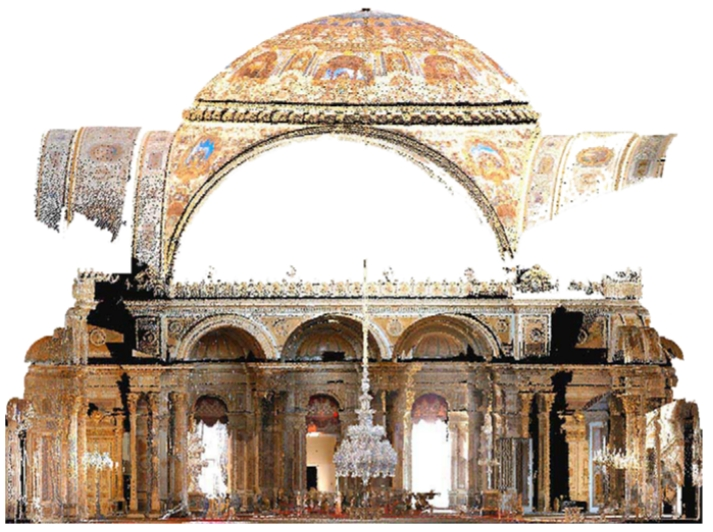
\includegraphics[width=6cm]{laser_scanning.jpg}
	\caption{Výstup dokumentace paláce Dolmabahçe - obarvené mračno bodů [50]}
\end{figure}

\chapter{Virtuální realita (VR)}
Cílem této kapitoly je seznámit čtenáře se základní definicí VR a její historií. Druhá část kapitoly je věnována VR v současné době, výčtu i porovnání zařízení a přehledu využití VR v různých oblastech.
\section{Definice VR}
Definovat VR je složité a stále neexistuje jednotná definice. To, co lze za virtuální realitu považovat, případně za její předchůdce, závisí na úhlu pohledu každého z nás. Různých definic existuje mnoho a značně se v klíčových oblastech překrývají. \\
Obecně však lze označit za VR takový soubor počítačového hardwaru a softwaru, který vizuální projekcí, zvukem a dalším působením na lidské smysly dokáže v co největší míře uživatele pohltit.[4] Jiná definice popisuje jako virtuální realitu trojrozměrnou simulaci prostředí, která je počítačově generována, za využití speciálního hardwaru.\\
\\
Pro VR jsou uváděny čtyři klíčové pojmy: virtual world, immersion, sensory feedback a interactivity. Na kvalitě či hodnotě těchto prvků stojí celkový dojem z VR.[1]\\
\\
Virtuální svět (virtual world) je to, jak virtuální realitu vnímá uživatel. Je vytvořen jeho smysly a může existovat, aniž by byl hardwarem zobrazován. Virtuální svět, který zrovna zařízení nezobrazuje, je popsán v příslušném skriptu, stejně jako tomu je například u her nebo filmů. Virtuální svět je tedy imaginární prostor prezentovaný VR.[1]\\
\\
Druhým klíčovým pojmem je ponoření (immersion). Tento prvek je částečně měřítkem, jak moc je uživatel obklopen virtuálním světem. Ponoření má také za úkol uživatele do imaginárního světa uvést tak, aby si toho byl vědom co nejméně. \\
Příklad: pokud je vytvořen ve VR model budovy s krajinou, je velmi důležitá úroveň detailů textur, fyziky prostředí i možnost interakce. Jsou-li tyto a další prvky na vysoké úrovni, je pravděpodobné, že uživatel bude značně ponořen do tohoto světa. V případě odstranění textur z modelu virtuálního světa bude uživatel ponořen méně.\\
Význam ponoření je tedy míra jakéhosi vcítění se uživatele do virtuálního prostředí. Pojem ponoření lze použít dvěma způsoby: mentální a fyzické. U většiny médií bývá zdůrazňováno ponoření mentální, a to ve smyslu emocionálního zapojení uživatele. U VR je téměř stejně důležité i fyzické ponoření. Fyzické ponoření je schopnost systému VR nahradit nebo rozšířit stimul působící na smysly uživatele.\\
Tato definice ponoření je ovšem jedna z mnoha a v různých literaturách lze nalézt i značně odlišné vysvětlení této problematiky.[1]\\
\\
Smyslová zpětná vazba (sensory feedback) je třetí důležitou částí každé VR. Jako předchozí prvek ponoření, tak i smyslová zpětná vazba je důležitá z hlediska přesvědčivosti umělého prostředí. Na uživatele přímo působí smyslová zpětná vazba na základě jeho fyzické polohy. Okamžitá interaktivní zpětná vazba má za důsledek vysoké nároky na hardware zprostředkujícího zařízení (PC apod.). Pro smyslovou zpětnou vazbu je nutné, aby systém VR měl stále aktuální informace o pohybu a poloze uživatele. Tyto způsoby snímání pohybu uživatele budou obsahem následujících kapitol.[1]\\
\\
Míra interaktivity (interactivity) světa ve VR je schopnost virtuálních objektů a prostředí reagovat na akce uživatele. Uživateli dává interaktivita pocit zapojení do virtuálního světa, uživatel je tak svým jednáním schopen rozhodovat o změnách a akcích v něm. Interaktivita je tedy míra schopnosti ovlivnit virtuální svět prostřednictvím fyzických akcí uživatele.[1] \\
\\
Zohlednění těchto čtyřech složek pro vysvětlení, co je VR, poskytuje vhodnou definici: Virtuální realita je médium složené z interaktivních počítačových simulací, které jsou schopny reagovat na polohu a akce uživatele, nahrazuje nebo rozšiřuje 
zpětnou vazbu působící na jeden nebo více smyslů.[1]

\section{Historie}
V roce 1838 popsal Sir Charles Wheatstone stereopsis  a v roce 1940 byl za vysvětlení binokulárního vidění vyznamenán královskou medailí. Tyto objevy jej dovedly ke konstrukci prvního stereoskopu. Jeho výzkum dokázal, že pozorováním kombinace dvou snímků stejného objektu, pořízených z různých úhlů z nenulové základny, vznikne vjem plastičnosti objektů na fotografiích. Každé oko přitom musí sledovat pouze jednu ze dvou fotografií. Wheatstoneův první stereoskop byl zkonstruován ze dvou zrcadel, natočených pod úhlem 45$^\circ$ vhledem k očím uživatele. Zrcadla odrážela obrazy umístěné stranou vzhledem k uživateli.[6]

\begin{figure}[h!]
	\centering
	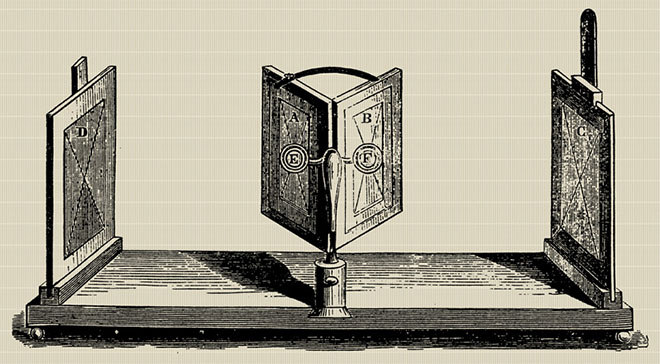
\includegraphics[width=9.5cm]{Wheatstoneův_zrcadlový_stereoskop.jpg}
	\caption{Nákres zrcadlového stereoskopu [4]}
\end{figure}

V roce 1935 spisovatel \textit{Stanley G. Weinbaum} vydal knihu \textit{Pygmalion's spectacles}. Sci-fi dílo, ve kterém hlavní postava využívá speciální brýle. Brýle přenášejí uživatele do smyšleného světa za pomoci holografických nahrávek a vhodné stimulace jeho smyslů. Z hlediska dnešní doby lze toto dílo považovat za první koncept VR, a to z důvodu správné predikce rozvoje tohoto oboru.[6]\\
\\
Za první přístroj, vytvářející a prezentující VR, je považována Sensorama. Stroj Sensorama vytvořil v roce 1956 kameraman Morton Heilig a patentoval jej v roce 1962. Prototyp při projekci krátkých filmů kombinoval trojrozměrné video, zvuk, vibrace, vůně a atmosférické jevy (vítr).[5] Trojrozměrný obraz byl tvořen stereoskopickou 3D obrazovkou. Autor konceptu považoval Sensoramu za kino budoucnosti a bylo vyvinuto šest krátkých filmů.\\
Heilig v roce 1960 také patentoval \textit{Telesphere Mask}. Jednalo se o první displej, který byl umístěn přímo na hlavu uživatele, neboli první \textit{head mounted display} (HMD). Tento přístroj poskytoval pouze trojrozměrné obrazy a zvuk, žádné sledování pohybu uživatele neexistovalo.[6]\\
\\
V roce 1965 představil počítačový vědec Ivan Sutherland svou vizi \textit{Ultimate Display}. Koncept představoval virtuální svět, který byl prohlížen prostřednictvím HMD. Realita měla být replikována na takové úrovni, aby ji uživatel nedokázal odlišit od skutečného světa. Zahrnuta tedy byla i interakce uživatele s objekty. Koncept obsahoval počítačový hardware, vytvářející virtuální svět, fungující v reálném čase. Tato vize je považována za základní plán VR.[6] Sutherland v poslední větě své vize přirovnává vhodně naprogramovaný \textit{Ultimate Display} k pohledu do Říše divů, kterou navštívila Alenka.[8]\\
\\
Vojenský inženýr Thomas Furness vytvořil v roce 1966 první letový simulátor pro výcvik pilotů. Pro VR má tento milník značný význam, protože armáda následně uvolnila velké množství finančních prostředků na zlepšení a další výrobu letových simulátorů.\\
\\První HMD pro VR vytvořil v roce 1968 Sutherland se svým studentem Bobem Sproullem. Co se týče uživatelského rozhraní, hardwaru i vizuálního zážitku bylo zařízení značně primitivní.  Grafika tvořící virtuální prostředí byla schopna prezentovat pouze jednoduché 3D objekty. Objekty měnily perspektivu v závislosti na pohybu hlavy uživatele. Hardware, který měl uživatel na sobě, musel být v důsledku vysoké hmotnosti zavěšen ze stropu. Vzhled byl inspirací pro pojmenování zařízení: The Sword of Damocles. [6]

\begin{figure}[h!]
	\centering
	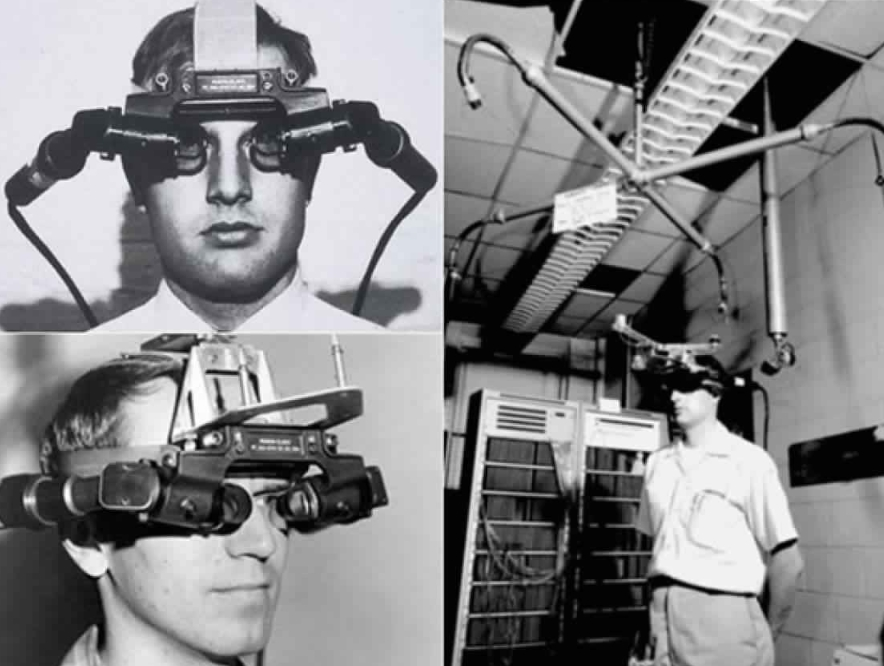
\includegraphics[width=6.5cm]{damoklův_meč.jpg}
	\caption{Zařízení nazývané Damoklův meč [56]}
\end{figure}

V roce 1969 vytvořil Myron Krueger řadu zážitků z umělé reality prostřednictvím počítačů a video systémů. Vytvořil počítačem generované prostředí, které reagovalo na pohyby uživatelů. Kruegerovo projekty byly počátkem technologie VIDEOPLACE. [6]\\
\\
V uměleckém centru Milwaukee byla roku 1975 umístěna první Kruegerova VIDEOPLACE paltforma (interaktiní virtuální realita). VIDEOPLACE využíval počítačové grafiky, projektory, videokamery a zařízení pro snímání polohy. Platforma fungovala zcela bez brýlí a rukavic. VIDEOPLACE byl vytvořen v temných místnostech s velkými obrazovkami, které uživatele obklopovaly. Uživatelé mohli vidět své, počítačem generované, siluety kopírující jejich pohyby a akce. Snímání pohybu bylo realizováno záznamem na kameru. Uživatelé v různých místnostech spolu mohli interaktivně provádět úkony ve virtuálním světě. Tento fenomén povzbudil myšlenku komunikace ve virtuálním světě bez nutnosti fyzické blízkosti.[6]\\
\\
Světově proslulý MIT (Massachusettský technologický institut) vydala v roce 1977 virtuální mapu Aspenu v Coloradu. Jednalo se o virtuální prohlídku podobající se dnešnímu Google Street View. Mapa byla vytvořena pomocí fotografií pořízených z auta projíždějícího městem. Pro tento virtuální model existovaly tři režimy prohlížení: léto, zima a mnohoúhel-níky. Hardware neobsahoval žádný HMD. Přínos tohoto projektu spočívá v myšlence přenosu uživatele na vzdálená místa bez nutnosti fyzického cestování.[6]\\
\\
První datové rukavice pro sledování gest uživatele vytvořili v roce 1982 Sandin a Defanti.[6] Sledování pohybu prstů bylo realizováno na bázi ohebných trubic, vybavených zdrojem světla na jednom konci a fotobuňkou na konci druhém. V závislosti na ohybu prstů se množství světla dopadající na fotobuňku měnilo a tím udávalo míru ohnutí. S tímto nápadem sledování pohybu přišel Richard Sayre, po kterém je zařízení pojmenováno.[9]\\
\\
Jaron Lanier a Thomas Zimmerman založili v roce 1985 společnost VPL Research. VPL Research vyvinula mnoho zařízení pro VR, například DataGlove, EyePhone HMD nebo Audio Sphere. Tato společnost byla první, která prodávala brýle a rukavice pro VR.[6]\\
\\
Mezi lety 1986-1989 vyvinul Thomas Furness letecký simulátor známý jako Super Cockpit. Výcvikový kokpit přenášel počítačem generované trojrozměrné modely i zvuk v reálném čase. Zařízení bylo vybaveno také sledovacím systémem přilby, který umožňoval uživateli ovládat simulátor pomocí gest, řeči i pohybu očí.[6]\\
\\
Scott Foster, zakladatel společnosti Crystal River Engineering, získal v roce 1989 smlouvu na projekt Virtual Environment Workstation Project, který byl pod záštitou NASA. Projekt byl zaměřen na vývoj výcvikového simulátoru pro astronauty ve VR. Společnost Crystal River Engineering vyvinula binaurální 3D zpracování zvuku v reálném čase.[6]\\
\\
Antonio Medina, vědec NASA, navrhl v roce 1991 systém VR pro ovládání robotických roverů na Marsu v předpokládaném reálném čase, a to navzdory zpoždění signálu způsobeným vzdáleností mezi planetami.\\
V tomto období byly přivedeny na trh také první arkádové automaty využívající VR. Hráči byli přeneseni prostřednictvím HMD do virtuálního světa. Některá zařízení disponovala propojením v reálném čase s ostatními. Uživatelé tak mohli hrát hry pro více hráčů. Tento první hromadně vyráběný herní VR systém vytvořila skupina Virtuality.\\
Společnost SEGA oznámila počátkem devadesátých let, že se zabývá vývojem soupravy SEGA VR, která bude cílena na širokou veřejnost. Tato náhlavní souprava byla určena pro arkádové hry na konzoli Mega Drive. Vzhled byl inspirovaný populárními filmy RoboCop apod.. HMD obsahoval LCD displeje, stereofonní sluchátka a senzory pro sledování pohybu hlavy. Navzdory již čtyřem vytvořeným hrám nebyl projekt nikdy dokončen.[6] Až v roce 1994 vydala společnost SEGA VR-1 (velký simulátor pohybu, který se otáčí v souladu s tím, co je promítáno na obrazovku).[10]\\
\\
Roku 1995 představila firma Nintendo herní konzoli Virtual Boy. Na konzoli bylo možné hrát trojrozměrné monochromatické videohry. Jednalo se o první přenosné zařízení zobrazující 3D grafiku svého druhu. Produkce konzole byla již po roce ukončena, uživatelé nebyli spokojeni s nedostatkem barevné grafiky a software neměl dostatečnou podporu.\\
Současně byly představeny nové soupravy pro VR, který byly určeny pro domácí využití: I-brýle od společnosti Virtual IO a VFX1 Headgear od společnosti Forte. [6]\\
\\
Vědci z Georgia Tech and Emory University využívali VR pro vytvoření scénářů v prostředí válečných zón ve Vietnamu. Tento projekt sloužil jako forma expoziční terapie PTSD(post-traumatické stresové poruchy) pro válečné veterány.[6]\\
\\
V roce 2001 se SAS3 nebo SAS Cube stala první kubickou místností založenou na PC, vyvinutou společností ZA Production. Knihovna SAS byla počátkem Virtools VRPack\footnote{\textit{\uv{Doplňková knihovna pro aplikaci Virtools Dev - vývojová platforma pro 3D vizualizaci.}}}.\\
\\
Společnost Google představila v roce 2007 Street View. Jedná se o virtuální prohlížení skutečného světa, vytvořeného z panoramatických snímků. Celý obsah se skládá ze dvou zdrojů: Google a samotní uživatelé.[12] Následně roku 2010 spustil Google stereoskopický 3D režim pro Street View.\\
\\
V období okolo roku 2010 vytvořil Palmer Luckey, osmnáctiletý podnikatel, první prototyp náhlavní soupravy Oculus Rift. Zorné pole zařízení bylo 90$^\circ$. Tento projekt obnovil zájem o vývoj VR. \\
Luckey zahájil kampaň na Kickstarteru pro Oculus Rift v roce 2012,ve které se podařilo získat 2.4 miliony dolarů. Přelomový byl pro společnost Oculus VR rok 2014. V tomto roce koupila společnost za 2 miliardy dolarů Facebook. Teto krok byl rozhodující pro budoucnost VR. \\
Téhož roku společnost Sony oznámila, že pracuje na projektu Morpheus neboli headsetu VR pro PlayStation 4. Google vydal Cardboard (do-it-yourself stereoskopický prohlížeč pro smartphony). Společnost Samsung představila Samsung Gear VR, náhlavní soupravu, která používá prohlížeč Samsung Galaxy. Mnoho dalších společností a odborníků se v tomto období začalo zabývat možnostmi VR, včetně přídavných inovativních doplňků.[6]\\
\\
V roce 2015 již začala být VR běžná mezi širokou veřejností. Wall Street Journal spustil VR roller coaster, který sledoval vzestupy a pády na akciovém trhu Nasdaq. BBC vytvořilo 360$^\circ$ video, kde uživatelé měli možnost sledovat syrský migrační tábor. Mediální společnost RYOT promítala krátký VR film o uvěznění v amerických věznicích. Projekt Gloveone, zaměřen na vývoj rukavic pro VR, byl úspěšný ve své kampani na Kickstarteru. Tyto rukavice umožňují uživatelům interakci s virtuálními objekty.[6]\\
\\
Do roku 2016 vyvíjely VR produkty stovky společností. Většina HMD měla dynamický binaurální zvuk. Společnost HTC vydala headset VIVE SteamVR. VIVE SteamVR bylo prvním komerčním vydáním VR zařízení se senzorovým sledováním polohy, které umožnilo uživatelům volně se pohybovat ve virtuálním prostoru.

\begin{figure}[h!]
	\centering
	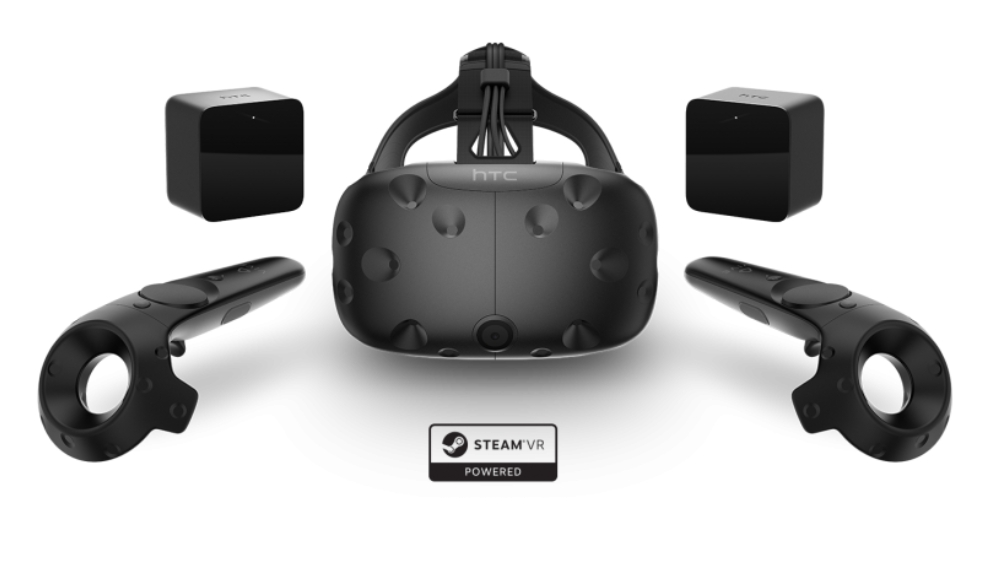
\includegraphics[width=16cm]{vive_steam.jpg}
	\caption{HTC VIVE SteamVR [57]}
\end{figure}

\section{Metody sledování pohybu}
Kromě širokého zorného pole se náhlavní soupravy pro VR liší od běžných 3D displejů tím, že jsou sledovány v prostoru. PC VR, konzolové VR a nyní i některé samostatné náhlavní soupravy mají polohové sledování. Sledování zařízení umožňuje uživateli se ve virtuálním světě volně pohybovat.[16]\\
\\
Většina mobilních zařízení pro VR má pouze rotační sledování neboli tři stupně volnosti (3DoF). Uživatel se může dívat nahoru a dolů, doleva a doprava nebo naklonit hlavu. Ale pokud se bude uživatel pohybovat, celý virtuální svět se bude pohybovat s ním. Tento způsob sledování pohybu neumožňuje uživateli se například procházet virtuálním světem nebo s ním přímo interagovat. Moderní VR zařízení jsou vybavena pozičním sledováním neboli šesti stupni volnosti (6DoF). Poziční sledování umožňuje uživateli se skutečně pohybovat ve virtuálním prostředí. Pokud disponují ovladače také 6DoF, může uživatel přímo interagovat s virtuálními objekty prostřednictvím rukou.\\
\\
Sledování rotace je obvykle u většiny výrobců prováděno prostřednictvím mikroskopických elektromechanických gyroskopů. Společnosti však používají rozdílné technologie ke sledování polohy zařízení.\\
\\
Jednotná primární metoda sledování u většiny VR systémů spočívá v kombinaci mikroskopických elektromechanických akcelerometrů obsažený v \textit{IMU} společně s \textit{MEMS} snímači úhlů. Výstupní veličinou akcelerometru je zrychlení. Pokud je zrychlení derivováno přes čas, výslednou veličinou bude rychlost ($v=\int a \cdot dt$). Dále pak lze získat integrací rychlosti přes čas polohový vektor ($r=\int v \cdot dt$). Sledování založené na akcelerometru a výpočtu jeho polohy se během několika sekund posunuje k nekonečnu. Důvodem je užití dvojité integrace, chyby se při výpočtu hromadí. Účelem sledovacích systémů je opravit posun vypočtený na základě dat z \textit{IMU}.

\subsection{Constellation}
Metoda sledování nazývaná Constellation byla použita u VR zařízení Oculus Rift. Každé sledované zařízení má předdefinovanou konstelaci IR LED diod. Senzory, kterými jsou kamery s filtry pro zobrazení pouze v IR oblasti záření, odesílají obrazová data do počítače. Počítač zpracovává snímky a identifikuje polohu každé diody, určuje tak relativní polohu objektu. Software dokáže snadno rozpoznat, které LED diody jsou viditelné, protože zná tvar konstelace, pamatuje si, kde byl objekt na předchozím snímku. Známá jsou také data z akcelerometru (zrychlení) a gyroskopu (rotace). Každá dioda bliká na jiné frekvenci, aby byla identifikovatelná.

\subsection{PlayStation VR}
PlayStation VR používá také kamery, ale na rozdíl od Oculus Rift pracuje ve spektru viditelného záření. Panel pro zařízení PlayStation 4 obsahuje dvě kamery. Kamerová jednotka je připojena ke konzoli, která používá obrazová data ke sledování barevných pruhů světla na náhlavní soupravě a ovladačích.

\subsection{Lighthouse}
Systém Valve SteamVR Lighthouse je v  využíván produkty HTC Vive. Na rozdíl od většiny ostatních systémů nepoužívá kamery vůbec. Systém je navržen tak, aby umožňoval polohové sledování v měřítku místnosti, aniž by bylo nutné vracet data ze základnových stanic do počítače. Základnové stanice jsou umístěny v protilehlých horních rozích místnosti. Nekomunikují s PC a nenesou senzory. Vyzařují širokoúhlý dvourozměrný IR laserový paprsek přes celou místnost, který tzv. zametáním postupuje celým prostorem po dobu 10 ms. Paprsek je vyzařován postupně po jedné a poté po druhé ose, tedy opakovaně v horizontálním a následně ve vertikálním směru. Před každou změnou osy vyzařování vyzařují silný IR záblesk světla. Každé sledované zařízení obsahuje řadu IR fotodiod připojených k čipu. Tento čip měří čas mezi IR zábleskem a zásahem objektu laserovým 2D paprskem pro každou osu. Tímto způsobem určuje polohu zařízení v místnosti.

\begin{figure}[h!]
	\centering
	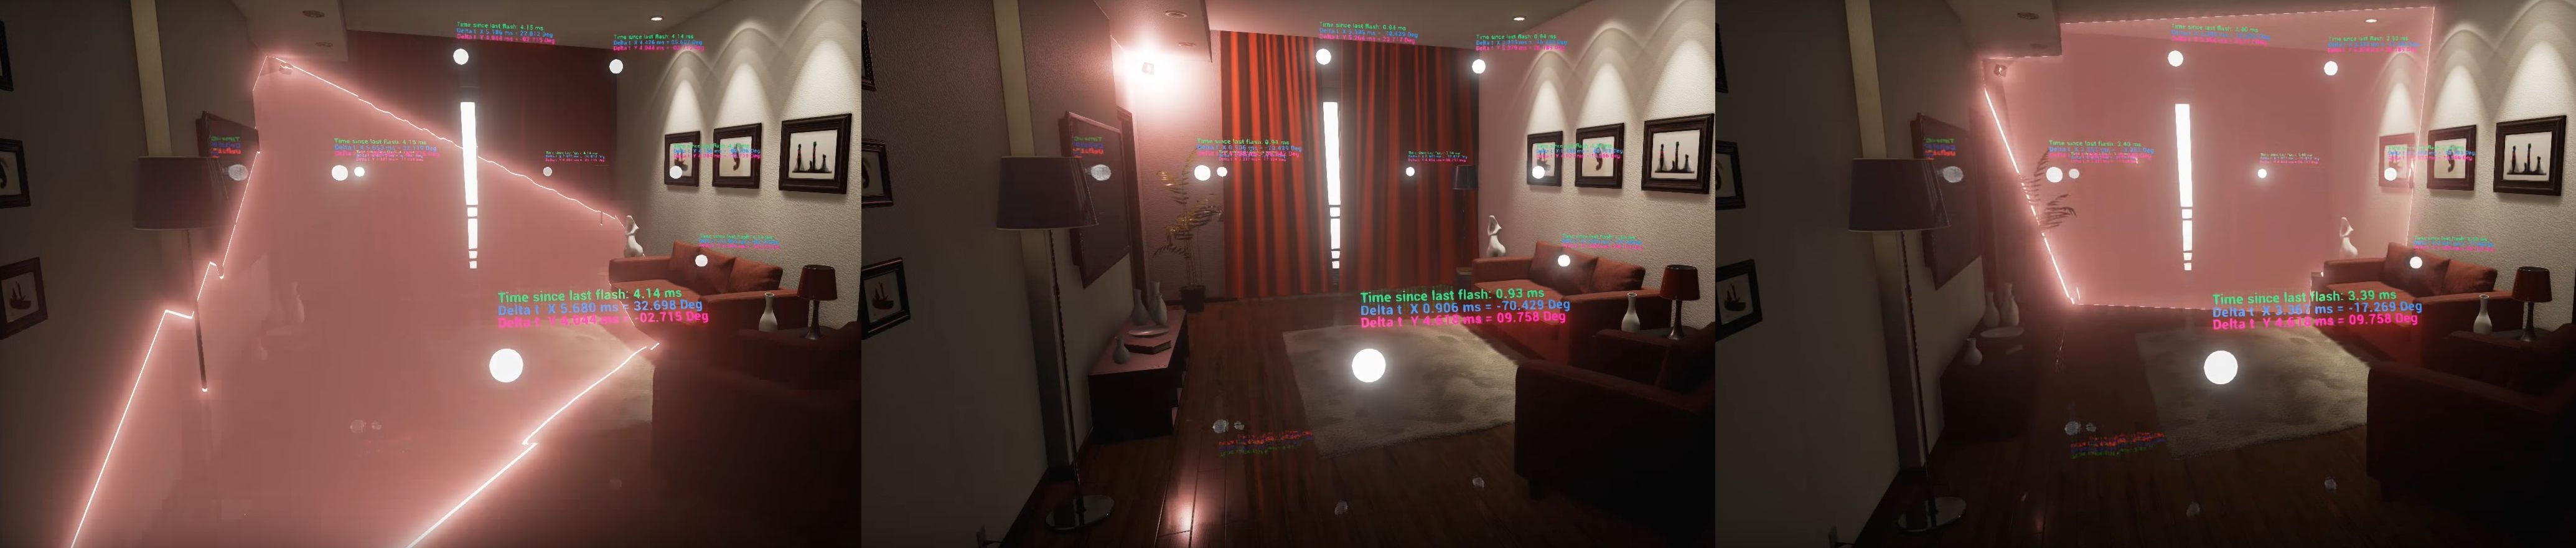
\includegraphics[width=16cm]{VIVE_laser.jpg}
	\caption{Model postupného vyzařování IR paprsku základní stanicí. [zdroj: 15]}
\end{figure}

\subsection{Inside-Out}
Mnoho VR zařízení používá fotoaparáty zabudované přímo do headsetu, které vyhodnocují polohu pomocí algoritmů počítačového vidění. Tento způsob sledování pohybu zařízení je označován jako inside-out. Algoritmus používaný pro vyhodnocení polohy je SLAM. Algoritmus SLAM funguje tak, že kamery zaznamenávají jedinečné statické prvky v místnosti. Porovnáním rotace a zrychlení s tím, jak se zaznamenané prvky pohybují, lze určit polohu headsetu.[16]\\
\\
\textit{Obecný proces při použití SLAM algoritmu:}
\begin{enumerate}
\item Přibližný odhad pozice zařízení - odometrie
\item Měření okolního prostředí - laserový skener
\item Vyhledání orientačních bodů v okolí na základě předchozího měření
\item Porovnání aktuálních bodů s uloženými v paměti z předchozích měření
\item Výpočet změny polohy zařízení z porovnání bodů 
\item Uložení nově pozorovaných bodů do paměti [21]
\end{enumerate}

%\subsection{Objektivy pro VR}
%Veškeré HMD pro VR v současné době nesou v krytu blokujícího okolní světlo dvě věci: obrazovku, která zobrazuje virtuální svět a sadu čoček nacházející se před touto obrazovkou.%

\section{Hardware VR v současnosti}
Hardwarové vybavení pro VR se v současnosti obecně skládá ze tří hlavních prvků: 
\begin{enumerate}
\item PC/konzole/smartphone
\item headset
\item ovladače a senzory.
\end{enumerate}

Jako výpočetní prvek pro zpracování a vykreslení obsahu VR lze použít chytrý telefon. Jedná se o nejekonomičtější variantu, která je spíše provizorním řešením zprostředkování VR. Headset obsahuje pouze slot pro umístění chytrého zařízení a vše ostatní obstarává telefon.\\
Tato možnost je zmíněna pouze pro celkový přehled o možnostech VR a nebude v této práci nadále zmiňována.\\
\\
Předpoklad funkčnosti vysoce kvalitního VR zařízení je hardwarově silný počítač nebo konzole. Hardwarové nároky na zařízení se obecně u každého výrobce VR liší. Další proměnnou je aktivita, která bude s headsetem vykonávána. Jedná-li se o zařízení fungující na výpočetním výkonu konzole a nikoliv PC, uvádí výrobce pro jakou verzi konzole je VR zařízení optimalizováno. \\
\\    
V roce 2020 se na trhu pohybuje mnoho VR zařízení všech typů (využívající výpočetní kapacitu počítače, konzole, samostatný HMD atd.). Mezi nejvýznamnější výrobce běžně dostupných zařízení pro VR patří HTC, Oculus, Sony a Valve. 

\subsection{HTC Vive}
První zveřejnění projektu Vive, na kterém se podílí společnosti HTC (Taiwan) a Valve (USA), bylo v roce 2015. V současné době se pod názvem Vive skrývají čtyři hlavní produkty: Vive, Vive Pro, Vive Cosmos  a Vive Focus.\\

\subsubsection{HTC Vive} Kompletní hardware pro VR obsahuje sluchátka, dva ovladače, dvě základnové stanice a headset. HTC Vive není napájeno samostatně, zařízení využívá výpočetní výkon počítače. \\
\\
Snímání pohybu uživatele je realizováno optickou cestou. Součástí kompletního vybavení jsou dvě základnové stanice. Stanice musí být umístěny v protilehlých rozích místnosti.[16] Výhodou této metody je jednoduchost algoritmu pro výpočet polohy. Základnové stanice nevyžadují propojení s PC, nutné je pouze napájení. Další výhodou je vysoká přesnost určování polohy v čase a široké pole sledování. Nevýhodou jsou vyšší náklady na výrobu, nutnost montáže základnových stanic a citlivost zařízení na reflexní povrchy. Metoda je obsahem kapitoly 4.3 Lighthouse.[16]\\
\\
U HTC Vive se nachází 32 fotodiod přímo na HMD se sluchátky a 24 na obou ovladačích. Fotodiody ochraňuje vnější skořepina obsahující IR filtry. Fotodiody jsou rozmístěny tak, aby byl výpočet polohy možný v jakémkoliv úhlu držení ovladače nebo HMD.[17] Sledování pohybu ovladačů napomáhá také šestiosá jednotka MPU-6500 společnosti InvenSense, kombinující tří-osý gyroskop a akcelerometr.[19]\\
\\
Headset HTC Vive obsahuje dva displeje Samsung AMOLED (447 ppi) s rozlišením 1080x1200 pixelů na jedno oko, kombinované rozlišení je pak 2160x1200 pixelů. Obnovovací frekvence je 90 Hz. Zorné pole displejů je 100$^\circ$ ve směru horizontálním a 110$^\circ$ ve směru vertikálním. Na displeje je pohlíženo přes Frenselovy čočky. Pro vstup je možné použít sloty: HDMI, USB 3.0 nebo 3.5 mm jack. Headset je vybaven Bluetooth a také kamerou od firmy Sunny Optical Technology. Ovladače jsou napájeny Li-poly baterií o kapacitě 960 mAh a napětí 3.85 V.[19] 

\begin{tabbing}
    RAM ~~\= 
    \= 34 \kill
    \bfseries Minimální hardwarové požadavky na PC pro HTC VIVE Pro \> \\[1mm]
    OS: \> Windows 7, Windows 8.1, Windows 10\\
    CPU: \> Intel Core i5-4590 nebo AMD FX 8350 nebo vyšší\\
    RAM: \> 4 GB\\
    GPU: \> NVIDIA GeForce GTX 1060 / AMD Radeon RX 480 nebo vyšší\\
    \end{tabbing}

\subsubsection{HTC Vive Pro} Headset HTC Vive Pro je podobný nižší verzi HTC VIVE. Hlavní rozdíly jsou ve vyšším rozlišení displejů, dvou objektivech kamery na předním krytu a vylepšené ergonomii. Verze VIVE PRO Eye obsahuje také zařízení pro sledování pohybu očí (Eye-tracker).[20]\\
\\
HTC Vive Pro je vybaven dual AMOLED displayem o rozlišení 1440x1600 pixelů na jedno oko. Výsledné rozlišení je tedy 2880x1600 pixelů. Display dokáže zobrazit 615 ppi. Tyto parametry vylepšují celkovou vizuální podobu virtuálního světa. Zařízení také disponuje funkcí pixel boost, který usnadňuje čtení textů. Hardwarové nároky na PC jsou stejné jako u HTC Vive.[20]\\
\\
HTC Vive Pro je vybaven integrovanými sluchátky s certifikátem Hi-Res. Sluchátka poskytují 3D prostorový zvuk. Headset obsahuje i duální mikrofon pro aktivní potlačení okolního šumu a aktivaci režimu konverzace nebo výstrahy. Uživatel má možnost i s nasazeným HMD komunikovat bez problému s okolím.[20]\\
\\
Duální kamera umožňuje základní sledování pohybu rukou bez nutnosti dalšího hardwaru. Jedná se o stereoskopický fotoaparát s rozlišení VGA. Dalším účelem je zachycování hloubkových dat do vzdálenosti dvou metrů a vylepšovat tak ochranné funkce.[20]

\begin{tabbing}
    RAM ~~\= 
    \= 34 \kill
    \bfseries Minimální hardwarové požadavky na PC pro HTC VIVE Pro \> \\[1mm]
    OS: \> Windows 7, Windows 8.1, Windows 10\\
    CPU: \> Intel Core i5-4590 nebo AMD FX 8350 nebo vyšší\\
    RAM: \> 4 GB\\
    GPU: \> NVIDIA GTX 970 / AMD Radeon R9 290 nebo vyšší\\
    \end{tabbing}

\subsubsection{HTC Vive Cosmos} Model Cosmos je vybaven osmi sledovacími kamerami. Kamery umožňují 310$^\circ$ pole sledování s šesti stupni volnosti. Kamery umožňují sledování pohybu a polohy zařízení bez nutnosti instalace základen. Cosmos je vybaven také integrovanými sluchátky s 3D prostorovým zvukem. Duálním displayem s rozlišením 1440x1700 pixelů na oko (celkové rozlišení činí 2880x1700 pixelů). Maximální zorné poje je 110$^\circ$. Další parametry jsou stejné jako u předchozích modelů.[20]

\begin{tabbing}
    RAM ~~\= 
    \= 34 \kill
    \bfseries Minimální hardwarové požadavky na PC pro HTC VIVE Pro \> \\[1mm]
    OS: \> Windows 10\\
    CPU: \> Intel Core i5-4590 nebo AMD FX 8350 nebo vyšší\\
    RAM: \> 4 GB\\
    GPU: \> NVIDIA GTX 970 / AMD Radeon R9 290 nebo vyšší\\
    \end{tabbing}

\subsubsection{HTC Vive Focus} Jediný model, který nevyužívá výkonu PC. Headset využívá procesoru Qualcomm Snapdragon 835 v kombinaci s operačním systémem Android. Zařízení není určeno pro herní využití, cílovou skupinou je podnikový uživatel. Focus obsahuje dva ultrazvukově sledované ovladače, které podporují systém Inside-out 6DoF. Na AMOLED displej s celkovým rozlišením 2880x1600 pixelů již není pohlíženo přes inovativní čočky, poskytující lepší grafiku. Display o 110$^\circ$ FoV je překreslován frekvencí 75 Hz.[20]

\subsection{Oculus}
Oculus je od roku 2014 pod křídly společnosti Facebook. Současná nabídka zařízení Oculus pro VR obsahuje tři položky: Oculus Go, Oculus Quest a Oculus Rift S. Jednotlivé produkty jsou určeny pro různé způsoby využití.\\

\subsubsection{Oculus Go:} Jedná se o první zcela autonomní headset. Uživatel nastaví zařízení pomocí mobilní aplikace a okamžitě může Oculus Go využívat. Není potřeba žádné připojení k PC nebo mobilu, ani externí snímače pohybu. Součástí kompletního hardwaru je i ovladač Oculus. Nevýhodou Oculus Go je, že neobsahuje žádný systém sledování okolního prostředí, případně možnost vytvoření místnosti, ve které bude virtuální zážitek fungovat. Jinými slovy, Oculus Go nedisponuje 6DoF.\\
\\
Headset má technické specifikace podobné smartphonu. Obrazovka je 5,5 palcový LCD displej s rozlišením 2560x1440 (1280x1440 na oko), který je překreslován s frekvencí 60 Hz. Výpočetní výkon je zprostředkován procesorem Snapdragon 821 od Qualcomm a základní model zahrnuje 32 GB úložného prostoru, přičemž je možné pořídit verzi s 64 GB velkým úložištěm. Na display pohlíží uživatel přes Fresnelovy čočky. Oculus Go váží 468 gramů, téměř stejně jako nejnovější HTC Vive. Headset je vybaven integrovanými sluchátky, podporujícími 3D zvuk. K zařízení je možné připojit i externí sluchátka.[19]\\

\subsubsection{Oculus Quest} Jedná se o plně samostatný VR headset systém s možností sledování polohy a pohybu. Quest je určen především pro herní využití.\\
\\
Přední část náhlavní soupravy je vyrobena z tvrdého plastu a obsahuje čtyři širokoúhlé sledovací kamery. Povrchem zadní části je textil, poslední komponentou headsetu jsou upínací popruhy, které v sobě nesou zabudované prostorové reproduktory. K zařízení je možné připojit i externí sluchátka. Obsahem kompletního hardwaru jsou duální ovladače, které disponují sledováním pohybu rukou i prstů.\\
\\
Zařízení poskytuje sledování pohybu se šesti stupni volnosti. Sledování pohybu a okolního světa zajišťuje technologie Oculus Insight, je schopna prostřednictvím kamer analyzovat okolní objekty pro přesnou reprezentaci reálného světa uživatele. Tyto kamery mohou také předávat monochromatické video okolí na obrazovku. Analyzovány jsou hrany, rohy a výrazné prvky okolí, zařízení poté vytvoří 3D mapu hracího prostoru a kombinuje tato data s daty z gyroskopu a akcelerometru. Jedná se o způsob sledování polohy nazývaný Inside-Out. Poloha soupravy je obnovována jednou za milisekundu. Duální ovladače jsou vybaveny prstenem pokrytým infračervenými světly. Senzory v náhlavní soupravě tyto světla sledují a určují tak polohu ovladačů.[22]\\
\\
Zařízení je vybaveno OLED obrazovkou, která má rozlišení 2880x1600 (1440x1600 na oko) a obnovovací frekvenci 72 Hz. Na obrazovku je pohlíženo přes Fresnelovy čočky. Výpočetní výkon zajišťuje 4 GB RAM a procesor Qualcomm Snapdragon 835. Oculus Quest obsahuje dobíjecí sadu lithio-iontových baterií s kapacitou 3648 mAh. Jedná se o dvoučlánkovou baterii se jmenovitým napětím 3,6 V. Zařízení je k dispozici ve dvou variantách, lišících se ve velikosti interního úložného prostoru, a to 64 GB nebo 128 GB. Hmotnost náhlavního zařízení je 571 g.[23]

\begin{figure}[h!]
	\centering
	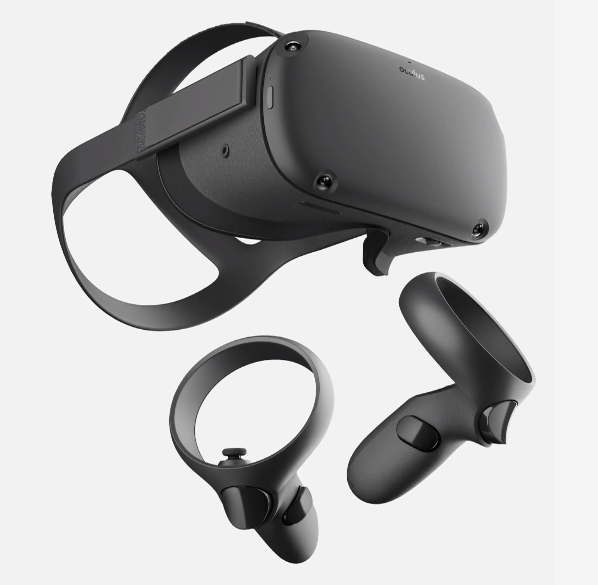
\includegraphics[width=9cm]{oculus.jpg}
	\caption{Oculus Quest [23]}
\end{figure}

\subsubsection{Oculus Rift S} Oculus Rift S je navazující model na předchozí Rift (Rift již není v nabídce firmy Oculus). Headset využívá výkon PC. Jedná se o nejkvalitnější zařízení pro VR, které je firmou Oculus nabízeno.\\
\\
Rift S obsahuje technologii Oculus Insight, která byla poprvé představena s modelem Oculus Quest. Díky pěti kamerám zabudovaným do náhlavní soupravy Rift S je Insight schopen převádět všechny objekty do virtuálního prostoru pro skutečnou reprezentaci fyzického světa. Jedná se opět o metodu Inside-Out, která je doplňována hodnotami z  gyroskopu, akcelerometru a magnetometru. Sledování pohybu rukou zde opět, jako u Oculus Quest, zajišťují dva ovladače vybavené infračervenými světly, které kamery na HMD sledují.[23]\\
\\
Rift S používá jeden LCD panel s rozlišení 2560x1440 a obnovovací frekvenci 80 Hz, který uživatel sleduje přes Fresnelovy čočky. Zorné pole je $115^\circ$ a souprava je vybavena nastavením  interpupilární vzdálenosti. Zvuk zajišťuje dvojice reproduktorů skrytá v pásku u uší. K zařízení lze připojit sluchátka přes 3.5 mm minijack. Zařízení Rift S obsahuje pouze dva kabely pro připojení: jeden USB 3.0 a jeden DisplayPort. Hmotnost headsetu je 561 g.[19]\\

\begin{tabbing}
    RAM ~~\= 
    \= 34 \kill
    \bfseries Minimální hardwarové požadavky na PC pro Oculus Rift S \> \\[1mm]
    OS: \> 64bitový Windows 10\\
    CPU: \> Intel Core i3-6100 / AMD Ryzen 3 1200, FX4350 nebo vyšší\\
    RAM: \> 8 GB\\
    GPU: \> NVIDIA GeForce GTX 1050Ti / Radeon RX 470 nebo vyšší\\
    \end{tabbing}
    
\subsection{PlayStation VR}
Systém virtuální reality, Sony PlayStation VR, je určen pro použití s herní konzolí \\ PlayStation 4 nebo PS4 Pro. Zařízení disponuje kvalitní a přesvědčivou VR s podporou sledování pohybu. Samotná náhlavní souprava je z velké části vyrobena z bílého plastu s výrazným zorníkem, který je nosičem většiny elektroniky, a jedním masivním čelním pásem, který slouží k upevnění zařízení na hlavě uživatele.[25]

\begin{figure}[h!]
	\centering
	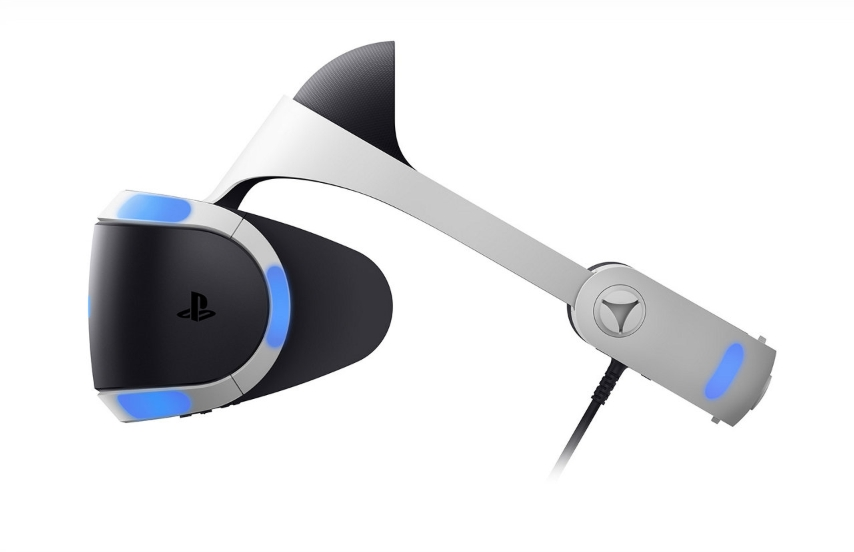
\includegraphics[width=10cm]{PS.jpg}
	\caption{PlayStation VR HMD [24]}
\end{figure}

Sedm šedých panelů umístěných na přední straně brýlí, společně s dvěma dalšími vzadu, skrývají barevná světla, která se rozsvítí při používání headsetu společně s kamerou PlayStation. Zařízení PlayStation Camera je vybaveno duálními objektivy a 3D hloubkovými snímači. Světla společně s kamerou zajišťují sledování polohy náhlavní soupravy i externích ovladačů DUALSHOCK 4, PlayStation Move nebo PlayStation VR aim. Metoda sledování pohybu je obsahem kapitoly 4.2 PlayStation VR.[24]\\
\\
Na OLED display s rozlišením 1920x1080 pixelů a rozměrem 5.7 palce pohlíží uživatel opět přes Fresnelovy čočky. Nejvyšší obnovovací frekvence displaye je 120 Hz. Uživatel je obklopen virtuálním světem se zorným polem o veliksoti 100$^\circ$. Pohyb ve virtuálním světě o šesti stupních volnosti zajišťuje společně s barevnými světly a kamerou také šestiosý systém detekce pohybu (tříosý gyroskop, tříosý akcelerometr). Propojení náhlavní soupravy společně s konzolí a televizí je zprostředkováno skrz externí procesorovou jednotku. Procesorová jednotka propojuje všechna zařízení prostřednictvím USB nebo HDMI kabelu. Zajišťuje 3D zpracování zvuku, zobrazuje sociální obrazovku (uzpůsobuje výstup VR pro zobrazení v televizi), zobrazuje softwarové rozhraní systému PS4 v filmovém režimu a zpracovává zobrazení tradičního 2D obsahu. Umožňuje také vývojářům posílat na připojenou obrazovku video výstup, zcela oddělený od toho, co vidí uživatel na HMD.[24]

\subsection{Valve Index}
Valve Index je souprava pro VR vytvořená a vyrobená společností Valve. Jedná se o vysoce kvalitní headset, který využívá výkon PC.\\
\\
Kompletní hardware pro Valve Index obsahuje dvě základnové stanice (umožňující sledování pohybu), dva ovladače a HMD na nejvyšší úrovni. Další částí jsou napájecí a připojovací kabely. Valve Index také zahrnuje dvojici nástěnných držáků pro základnové stanice. Hmotnost náhlavní soupravy je přibližně 800 gramů. Zařízení Valve Index má pevný, mechanicky nastavitelný upínací popruh. Zadní část popruhu obsahuje malý číselník, který řídí nastavení velikosti.\\
\\
Valve Index obsahuje inovativní integrovaná nepřímá sluchátka Balanced Mode Radiators, která jsou umístěna v blízkosti uší, ale nedotýkají se jich. Náhlavní souprava Valve má dva LCD displaye s rozlišením 1440x1600 pixelů na jedno oko (Valve nezveřejnil velikost panelů). Valve Index je první PC-VR náhlavní souprava, která nabízí panely, jež podporují obnovovací frekvenci 144 Hz. Společnost Valve navrhla pro objektiv vlastní dvouprvkové čočky. Společnost udává, že tyto čočky poskytují vysokou geometrickou stabilitu a minimální zkreslení tvaru. U objektivu zařízení je možné nastavit vzdálenost čoček od očí i vzdálenost čoček od sebe. Kombinace displejů a čoček umožňuje nastavení zorného pole až do rozměru $130^\circ$. Dvojice kamer, umístěna na předním krytu HMD, slouží k zobrazení reálného okolního světa.[26]\\
\\
Sledování zařízení zajišťují senzory SteamVR 2.0, kompatibilní se základnovými stanicemi SteamVR 1.0 a 2.0. Metoda sledování je uvedena v kapitole 3.3.3 Lighthouse. Dva dodávané ovladače Valve Indexu jsou zkonstruovány tak, aby je bylo možné pevně přichytit k ruce. Kombinace sledování pohybu prstů, kterým jsou ovladače vybaveny, a pevného upevnění na ruce umožňuje uživateli ve virtuálním světě například skutečně sbírat a upouštět předměty. Ovladače mají tlakové senzory, které detekují míru stisku ovládacích prvků uživatelem. Každý ovladač používá 87 senzorů různých typů: optických, pohybových, kapacitních a silových.[27]
\\
\\
Přední čelní deska náhlavní soupravy Index obsahuje odnímatelný panel, který zakrývá dutinu, kterou Valve nazývá „Frunk“. Výrobce nemá žádné specifické určení pro přední slot, ale umístil tam port USB, aby s ním mohli experimentovat vývojáři a výrobci hardwaru.[26]
 
\begin{tabbing}
    RAM ~~\= 
    \= 34 \kill
    \bfseries Minimální hardwarové požadavky na PC pro Valve Index \> \\[1mm]
    OS: \> Windows 10, SteamOS, Linux\\
    CPU: \> Dual Core s Hyper-Threading\\
    RAM: \> 8 GB\\
    GPU: \> Nvidia GeForce GTX 970 / AMD RX480\\
\end{tabbing} 

\begin{figure}[h!]
	\centering
	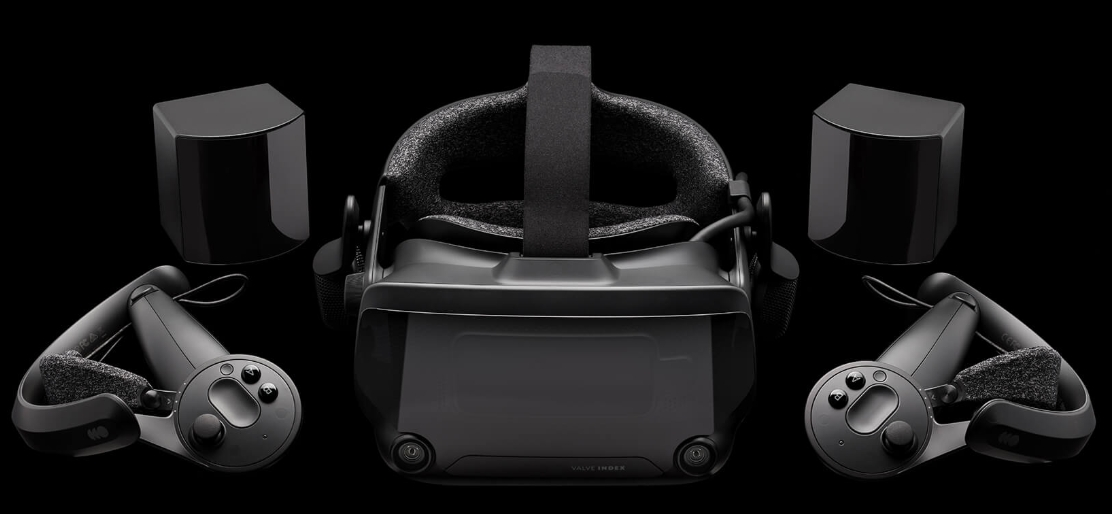
\includegraphics[width=16cm]{valve.jpg}
	\caption{Valve Index [27]}
\end{figure}

\section{Využití VR v současnosti}
V současné době je z médií nejvíce patrný rozvoj VR v oblasti zábavního průmyslu. Hraní her a zábava jsou ovšem pouze část z mnoha způsobů využití. Velmi důležitou úlohu má VR také v stavebním průmyslu, vojenství, automotive průmyslu, marketingu, zdravotnictví, vzdělávání a mnoha dalších oborech. Prudký rozvoj VR v současné době naznačuje, že oblasti využití se budou rychle rozrůstat a VR se v průběhu následujících několika let stane běžným prvkem každodenního života, jako je tomu dnes například u počítačů. V následujících podkapitolách jsou podrobněji popsány jmenované způsoby využití VR.

\subsection{Stavební průmysl}
VR ve stavebnictví je další úrovní 3D modelování. Vytvoření 3D modelu staveniště bývalo složitým fyzickým procesem, který byl nákladný na prostor, čas i materiály. Tyto miniaturní modely pomohly při organizaci projektu, ale nutně obsahovaly nepřesnosti a chyběly podrobnosti. 3D modelovací software umožnil nejen rychlejší a levnější vytvoření podrobného, přesného modelu, ale také sdílení těchto modelů. VR umožňuje uživateli ponořit se do projektu, jako by se tam fyzicky nacházel, a interagovat s prostředím přesně tak, jako by tomu bylo ve skutečnost.[30]\\
\\
VR umožňuje týmům snadnou spolupráci v reálném čase ve sdíleném virtuálním prostředí, kde mohou doslova poukázat na podrobnosti a problémy, klást otázky a okamžitě rozhodovat o změnách. Například nezisková organizace Build Change staví budovy po celém světě, včetně rozvojových zemí a oblastí náchylných ke katastrofám. Používají VR, aby pomohli zúčastněným porozumět potřebám projektu během fáze plánování a také aby mohli sledovat pokrok a poskytovat vstupy během fáze výstavby.[30]\\
\\
Během celého procesu výstavby umožňují zákazníkům aktualizované 3D modely v prostředí VR sledovat vývoj projektu a přesvědčit se, že vše postupuje podle plánu. Pokud vzniknou problémy a dotazy, mohou je zákazníci okamžitě řešit ve spolupracujícím virtuálním světě.[30]

\subsection{Vojenství}
Jak bylo již v kapitole týkající se historie patrné, je VR důležitým elementem vojenského výcviku již mnoho let. Simulace virtuálního světa spolu s interakcí umožňuje výcvik vojáků v jakémkoliv prostředí, bez nutnosti cestování a především bez jakéhokoliv rizika. VR umožňuje vojákům nácvik správných úkonů v krizových situacích a zároveň takový výcvik je méně nákladný než klasické metody. Vojenská využití VR zahrnují: letové simulace, simulace bojiště, zdravotnický trénink, simulace vozidla apod.\\
\\
VR se také používá k léčbě posttraumatické stresové poruchy. Vojáci, trpící traumatem z bojiště a jinými psychologickými stavy, se mohou naučit, jak se vypořádat s jejich příznaky ve virtuálním prostředí.\\
\\
Je zřejmé, že virtuální prostředí je ideálním prostředkem pro vojenský výcvik v tom, že umožňuje účastníkům, tj. vojákům, zažít konkrétní situaci v kontrolovaném prostoru. Například scénář bojiště, ve kterém mohou interagovat s událostmi, ale bez jakéhokoli nebezpečí. Dalšími výhodami jsou čas a náklady: vojenský výcvik je velmi drahý, zejména letecký výcvik, takže použití letových simulátorů je nákladově efektivnější než skutečná letadla. Navíc je možné zavést do scénáře výcviku prvek nebezpečí, aniž by však způsobil účastníkům skutečné fyzické poškození.

\subsection{Automotive průmysl}
V současné době je VR využívána v automobilovém průmyslu například v USA, Japonsku a Evropě. Téměř všechny hlavní automobilové podniky, jako jsou GM, Ford, Chrysler, Audi, Benz, Porsche, BMW, Volkswagen, Honda nebo Toyota používají VR v oblasti výroby i marketingu.[31]\\
\\
VR je používána ve všech oblastech automobilového průmyslu, jako jsou: styling, strojíren-ství,
proces výroby, testování nebo montáž. Poskytuje nejen vhodné prostředí pro inženýr-ské práce, ale také zlepšuje vývojový proces. Výhodou práce ve VR při tvorbě prototypu automobilu je možnost interakce a přímého kontaktu pracovníka s modelem bez nutnosti skutečné výroby prototypu. Nedostatky nebo změny lze ve virtuálním světě okamžitě objevit a opravit bez nutnosti nákladné přestavby prototypu. Ve VR je u mnoha automobilek testována i samotná montáž produktu. Takovéto metody výroby, založené na práci ve virtuálním světě, snižují výrobní náklady v řádech milionů.[31]\\
\\
Například v Mazdě může zákazník použít HMD a ve virtuálním světě měnit barvu automobilu i příslušenství. Automobilka Ford využívá VR například k simulaci údržby motorů.[31]

\subsection{Marketing}
Virtuální svět nabízí digitální zážitek místo fyzického, společnost tak může efektivně propagovat produkty a služby. Kromě propagace stávajících produktů slouží VR k předvedení prototypů, které jsou ve vývoji. Zákazník, který má možnost podílet se na tvorbě nových produktů skrz VR, poskytuje relevantnější zpětnou vazbu. Přístup zákazníka k produktu ještě před jeho vyhotovením jej přiměje do výrobku spíše investovat z důvodu možnosti vlastních úprav a vyzkoušení zboží.\\
\\
Například společnost Amazon v roce 2018 představila v Indii VR kiosky. Nasazený HMD přenese uživatele do virtuálního světa, ve kterém je dopraven horkovzdušným balónem do města plného obchodů. Zákazník má možnost se proházet virtuálním světem a interagovat se zbožím. Prostřednictvím soupravy Oculus Rift má možnost si uživatel nakoupit veškerý sortiment nabízený společností Amazon ve VR.[32]

\subsection{Lékařství}
Podle zprávy společnosti Grand View Research se očekává, že trh VR v oblasti zdravotnictví vzroste do roku 2025 na 5,1 miliardy dolarů. Ve zdravotnictví je VR využívána mnoha způsoby, od školení lékařů až po diagnostiku a léčbu různých stavů.[37]\\
\\
Dětská nemocnice St. Joseph v Tampě využívá  technologii VR k vytváření virtuálních modelů anatomie pacienta. Nemocnice používá  technologii Surgical Theatre Precision Virtual Reality k vytvoření modelů. Stejná technologie je používána pro simulaci stíhacích letadel F-16. Takovéto metody jsou v současné době používány pro oblasti neurologie a srdeční chirurgie. [33]\\
\\
Nedávná práce z University of Cambridge zjistila, že VR by mohla být účinnější při detekci rané Alzheimerovy choroby než tradiční kognitivní testy. Výzkum vychází z práce profesora Johna O'Keefe z University College London v roce 2014. [33]\\
\\
VR je také účinná při budování rovnovážných dovedností u pacientů s Parkinsonovou chorobou. Tento systém úspěšně zlepšil vyrovnání se pacienta s překážkami a důvěru v pohyb ve virtuálním prostředí. [33]\\
\\
Správné provedení operace je pro začínajícího chirurga velmi náročný úkol. Možnosti školení v rané fázi kariéry jsou omezené. V nejideálnějším případě měli první chirurgové možnost provést operaci na mrtvém těle před skutečným zákrokem, při kterém byla bezpečnost pacienta plně v jejich rukou.  Společnost Osso VR vyvíjí pomocí VR chirurgickou tréninkovou platformu pro simulaci mnoha druhů operací.[33]

\begin{figure}[h!]
	\centering
	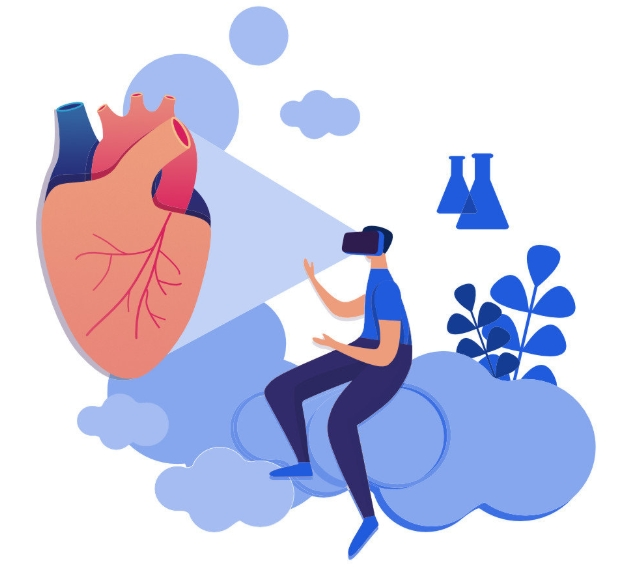
\includegraphics[width=9cm]{lekarstvi.jpg}
	\caption{Využití VR v lékařství [56]}
\end{figure}

\subsection{Vzdělávání}
Vzdělávání je další oblastí, která využívá VR. Výhodou je to, že umožňuje velkým skupinám studentů interagovat navzájem i v trojrozměrném prostředí. Virtuální svět je schopen studentům představit komplexní data, která jsou zábavná a snadno se učí. Studenti mohou interagovat s různými prvky virtuálního světa, aby se o nich dozvěděli více.\\
\\
Například se studenti astronomie mohou dozvědět o Sluneční soustavě přímo fyzickým zapojením se do virtuálního modelu. Mohou pohybovat planetami, vidět hvězdy a sledovat průlet komety. To umožňuje studentům vidět, jak jinak abstraktní pojmy fungují v trojrozměrném prostředí.\\
\\
Vzdělávání se posunulo od knih, sešitů a pera k využívání interaktivních technologií, které pomáhají zábavnou formou předávat znalosti.[34]

\subsubsection{Virtuální muzeum}
Muzea po celém světě se potýkají s problémy spočívajících v omezené kapacitě, riziku poškození exponátů nebo nadměrných nákladech na tvorbu a transport expozic. Některá muzea nejsou ochotna propůjčovat cenné exponáty pro výstavy mimo areál, ačkoliv takovéto exotické expozice jsou v dnešní době nejvíce oblíbené a zajišťují vysoký finanční příjem. VR i AR nabízejí ideální prezentační i vzdělávací médium suplující reálné muzejní expozice. Výhodou je také snadná dostupnost pro širokou veřejnost všech věkových skupin včetně zdravotně postižených jedinců apod.[34] Dalším zvýhodňujícím elementem pro muzeum ve virtuálním světě je možnost vysoké interakce jak s okolím, tak s exponáty bez nebezpečí poškození předmětů, krádeže nebo zranění osob.\\
\\
Virtuální výstavy lze vizualizovat formou standardního webového obsahu nebo na bázi VR či AR prezentace v integrovaném rozhraní koncového uživatele. Význam virtuálních muzeí ve vzdělání je vysoký pro oblasti, kde se potenciální návštěvníci nacházejí ve velké geografické vzdálenosti od muzejních center, která bývají zpravidla umisťována do hustě osídlených oblastí. Edukační význam tak mají virtuální muzea především pro polohově odloučené vzdělávací instituty rozsáhlých zemí (např. Rusko, Austrálie apod.). [35]\\
\\
V poslední době, kdy svět zasáhla pandemie Covid-19, jsou virtuální návštěvy často jedinou možností, jak navštívit kulturní objekty včetně muzeí.

\subsection{Zábavní průmysl}
Nejvíce rozšířený způsob využití VR v běžné společnosti jsou zábava a hry. Výrazný rozvoj VR v oblasti zábavního průmyslu je patrný již od samého vzniku prvních zařízení. Se zařízením určeným pro tento způsob využití lze hrát speciálně vytvořené hry, sledovat interaktivní filmy, dokonce jsou připravovány platformy sociálních sítí ve virtuálním světě. Jak je uvedeno v předchozích kapitolách, VR poskytuje uživateli ponoření do vybraného virtuální světa a společně se zpětnou vazbou na smyslové vnímání i interaktivitou prostředí je ideálním prostředkem pro zábavu.  

\begin{figure}[h!]
	\centering
	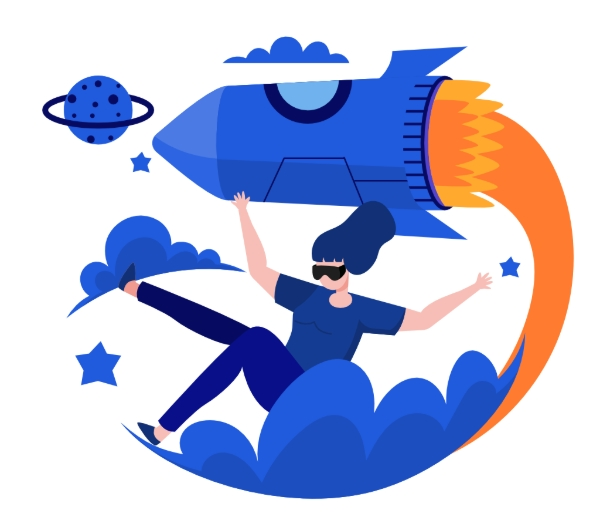
\includegraphics[width=9cm]{zabava.jpg}
	\caption{Využití VR v zábavním průmyslu [56]}
\end{figure}
 
\chapter{Image Based Modeling and Rendering}
IBMR technologie umožňuje tvorbu virtuálních 3D objektů z fotografických snímků. Jedná se o fotogrammetrickou metodu tvorby mračna bodů podobného tomu, které by vzniklo laserovým skenováním téhož objektu. Princip, kterým je získávána prostorová informace bodů na snímkách, se nazývá obrazová korelace. Postup tvorby hustého mračna bodů ze snímků metodou IBMR lze rozdělit do tří fází: sběr dat, extrakce řídkého mračna bodů a následně extrakce hustého mračna bodů.[28]\\
\\
\textbf{Sběr dat:} Při pořizování snímků za účelem následného zpracování metodou obrazové korelace je důležité dbát na velký překryv snímků (70-80\%), které by měly být konvergentní, je vhodné zařadit mezi data i přibližně stereoskopické snímky s rovnoběžnými osami záběru. Vliv na výsledný výstup mají také vnější podmínky, při snímkování je vhodné neměnit nastavení fotoaparátu, vzdálenost k objektu a osvětlení. Při pořizování dat by měla zůstat ohnisková vzdálenost fotoaparátu konstantní. Ačkoliv je pro klasickou fotogrammetrii vyžadováno vypnutí automatického ostření, není tento krok pro tvorbu mračna bodů metodou IBMR nezbytný. Software užívaný v současné době je napsán tak, aby byl vhodný i pro širší veřejnost a s tímto aspektem počítá. Program při zpracování dat vypočítá také změnu měřítka, způsobenou malou změnou ohniskové vzdálenosti objektivu při automatickém ostření.[29]\\
\\
\textbf{Extrakce řídkého mračna bodů:} Tvorba řídkého mračna bodů slouží pro výpočet prvků vnější a vnitřní orientace. Řídké mračno obsahuje body, které jsou v obraze dobře detekovatelné. Nejprve se na jednotlivých snímcích vyberou vhodné body, dalším krokem je tzv. matching neboli přiřazení bodů si navzájem. Princip je založen na obrazové korelaci snímků. Obecně je metoda založena na výpočtu korelačního koeficientu, který je počítán na základě pohybující se matice pixelů po části snímku, kde je předpoklad existence hledaného bodu. Hodnoty jsou počítány pro jednotlivé polohy vyhledávacího okénka. Je-li korelační koeficient dostatečně vysoká hodnota, software určí polohu matice jako pozici hledaného identického bodu. Stejné body, detekované na minimálně dvou snímcích (identické či spojovací body slouží při výpočtu analytické aerotrinagulace – AAT metodou komplexního řešení bloku fotografií. Výsledkem operace je společně s prvky vnější a vnitřní orientace také řídké prostorové mračno bodů.\\
\\
\textbf{Extrakce hustého mračna bodů:} Ze známých prvků vnější i vnitřní orientace a ze snímků vytvoří software za použití obrazové korelace husté mračno bodů, tj. pro všechny body na snímcích, pokud to lze, se počítá jejich prostorová poloha. Bodům je přiřazena textura a výsledkem celého procesu je texturované husté mračno bodů. \\
\\
Nárůst výkonu osobních počítačů zapříčinil výrazný nárůst využití IBMR technologie v běžné praxi. Pro data z RPAS (tzv. dronů) je IBMR hlavní metodou zpracování. Celý proces zpracování dat je ve většině softwarů plně automatický a není možné do výpočtu ve větší míře zasahovat. Výhodou technologie IBMR jsou nízké náklady na používanou techniku v porovnání např. s laserovým skenováním. V mnoha případech, a zejména u blízkých a menších objektů, je IBMR technologie tvorby hustého mračna bodů (a tedy jejich prostorová dokumentace) kvalitnější a detailnější, než při použití laserového skenování.  

\chapter{Tvorba virtuálního muzea}

\section{Tvorba modelu budovy}
Pro vytvoření základního modelu budovy muzea byl použit software \textit{SketchUp},který je v současné době vyvíjen společností \textit{Trimble}. Software umožňuje uživatelům vytvářet 2D i 3D modely pro použití v mnoha oborech, včetně architektury i herního průmyslu. Výhodou programu je intuitivnost a uživatelská přívětivost.[41] Pro tvorbu budovy byly použity pouze základní funkce programu, jako je například tvorba linií nebo nástroj \textit{Push/Pull} pro tvorbu 3D objektů z ploch.\\
\\
Model budovy byl navrhován tak, aby interiér nebyl příliš členitý a vyhovoval následnému využití jako muzeum. Budova obsahuje dvě patra propojená poschodím uvnitř. Vnější část disponuje vyvýšenou terasou a designovými elementy. Výrazným prvkem celého modelu jsou četná okna, která jsou důležitým prvkem pro osvětlení objektů ve virtuálním světě. Zvýšená pozornost při tvorbě jednotlivých částí objektu byla věnována orientaci jednotlivých ploch. Plochy, které mají být v následné vizualizaci viditelné, musí být nastavené jako přední. Plochy, které si nesou informaci opačnou, se v programu \textit{UE4} zobrazí jako průhledné. Výslednému modelu budovy byly přiřazeny základní textury, které jsou implementovány jako součást použitého softwaru. Export byl proveden do CAD formátu \textit{FBX}.

\begin{figure}[h!]
	\centering
	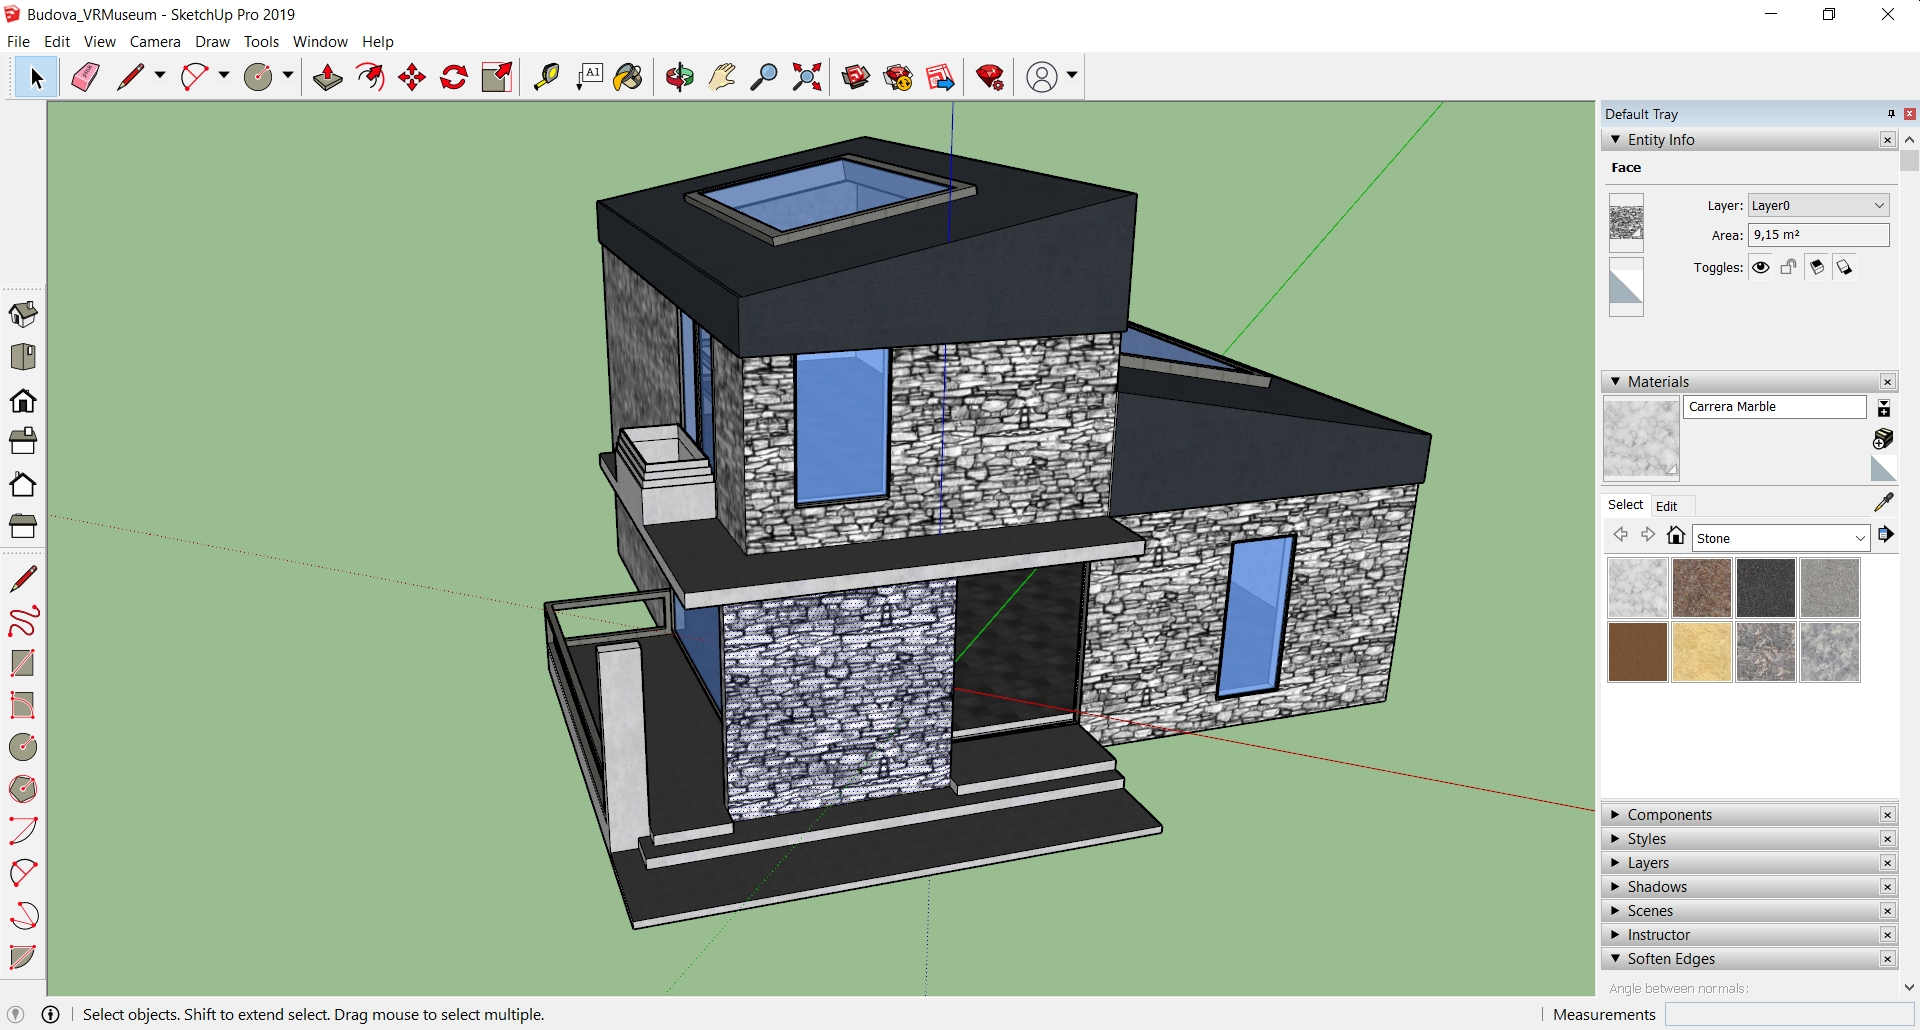
\includegraphics[width=11cm]{budova.jpg}
	\caption{Model budovy vyhotovený v softwaru \textit{SketchUp}}
\end{figure}

\section{Tvorba virtuálního prostředí}
Tvorba veškerého prostředí, včetně umístění všech potřebných objektů pro vytvoření kvalitního VR muzea, byla provedena v herním enginu \textit{Unreal Engine 4}. Produkt \textit{UE4} vytvořený firmou \textit{Epic Games} je vysoce kvalitní volně přístupný nástroj pro 3D tvorbu v reálném čase. Jádro softwaru je napsáno v programovacím jazyce \textit{C++}. Engine podporuje v současné době mnoho platforem a disponuje také možností vlastního skriptování při tvorbě nového obsahu.[42] V aplikaci \textit{Epic Games Launcher} umožňuje sekce \textit{Marketplace} stažení volně přístupného i placeného obsahu pro projekty vytvářené v \textit{UE4}.\\
\\
Prvním krokem pro vytvoření prostředí bylo založení nového projektu. \textit{UE4} nabízí čtyři kategorie pro vytvoření nového projektu: \textit{Games; Film, Television and Live Events; Architecture, Engineering and Construction; Automotive, Product Design and Manufacturing}. Vzhledem k povaze a účelům této práce byla zvolena kategorie \textit{Games}. Zvolená kategorie disponuje čtrnácti různými šablonami, včetně prázdné. Pro tvorbu prostředí, které má být prezentováno formou virtuální reality, byla zvolena stejnojmenná šablona. Šablona \textit{Virtual Reality} obsahuje připravené funkce a obsah pro tvorbu virtuálního prostředí bez nutnosti programování.\\
\\
Dalším krokem bylo vytvoření nového levelu v projektu. Implicitně připravený level, který se po spuštění projektu v \textit{UE4} zobrazí, nebyl vhodný pro účely této práce. Při tvorbě nového levelu: $File \rightarrow New Level...$, byla zvolena možnost $Default$. Zvolená možnost přidá do nově vytvořeného levelu základní prvky osvětlení, atmosféry a \textit{static mesh} s názvem \textit{Floor}. Veškerý tento základní obsah byl v průběhu tvorby prostředí odstraněn a nahrazen nově vytvořenými prvky.

\begin{figure}[h!]
	\centering
	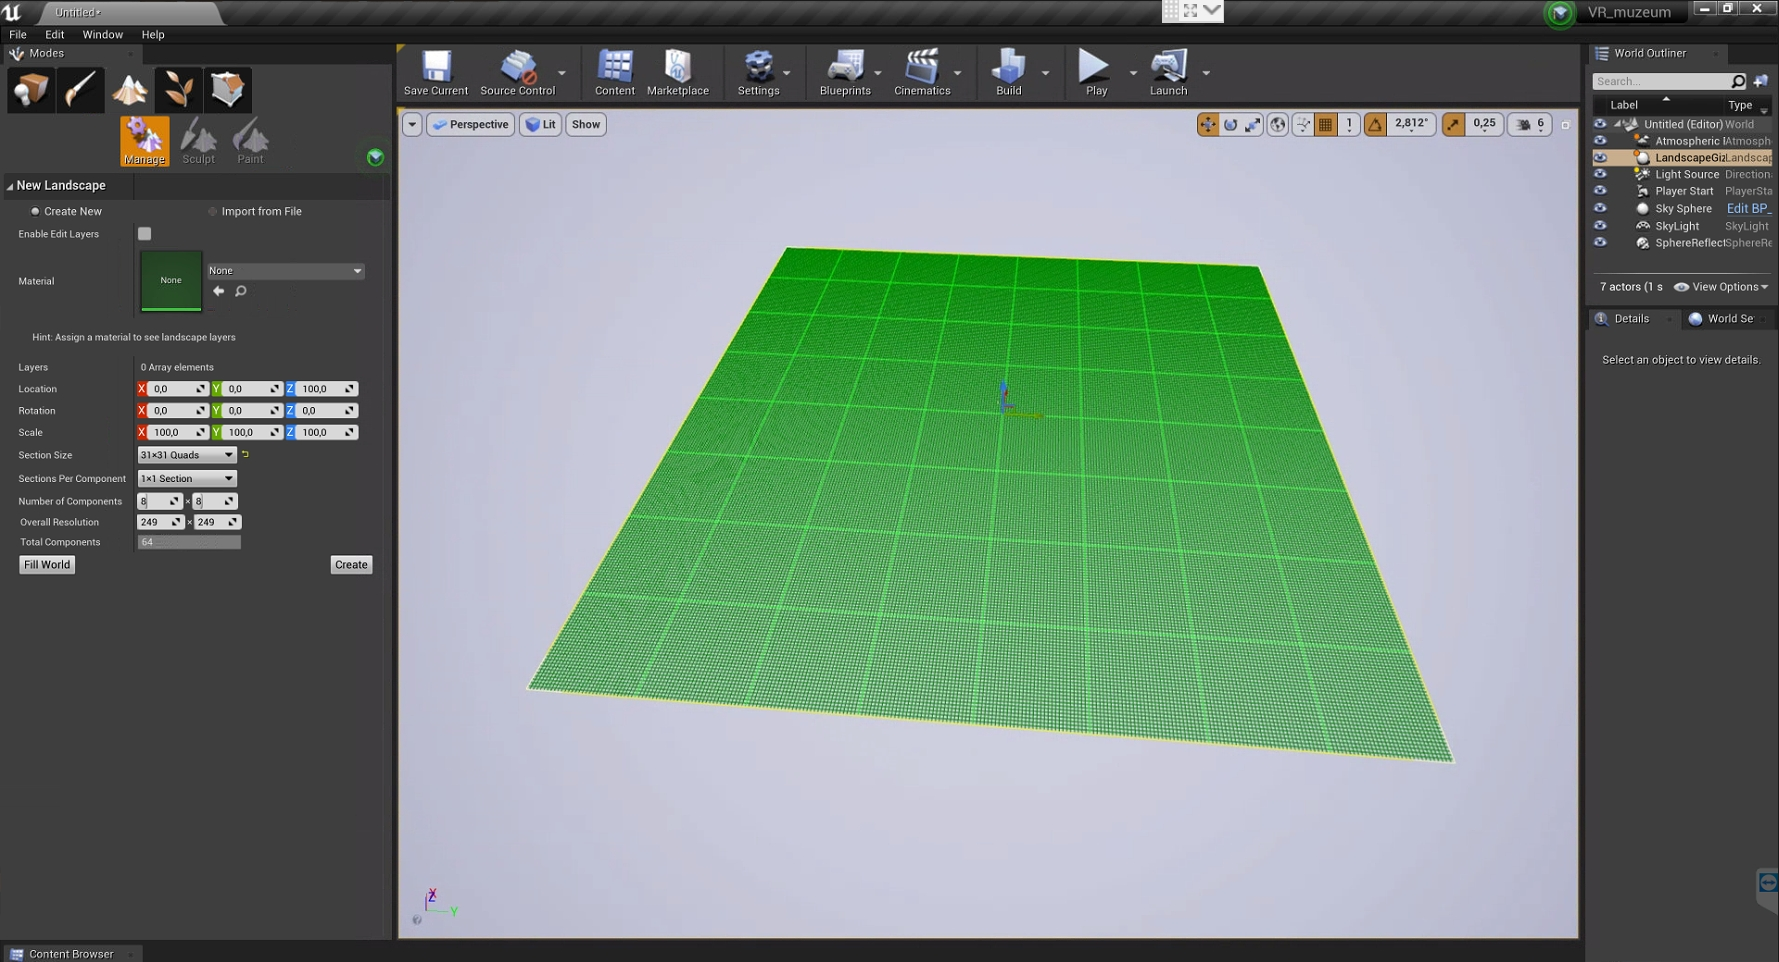
\includegraphics[width=16cm]{newLevel_settings.jpg}
	\caption{Tvorba a nastavení nové krajiny v \textit{UE4} }
\end{figure}

Pro tvorbu virtuální krajiny je v \textit{UE4} implementována funkce \textit{Landscape}. \textit{Landscape} disponuje třemi hlavními nástroji: \textit{Manage, Sculpt} a \textit{Paint}. Záložka s názvem \textit{Manage} obsahuje možnosti importu nebo vytvoření a nastavení nové virtuální krajiny. Model krajiny je v \textit{UE4} rozdělen do komponent (ve formě pravidelné čtvercové sítě), které jsou základní \textit{Unreal} jednotkou pro vykreslování, výpočet viditelnosti a kolize. Pro projekt byl nastaven počet komponent na $8\times8$. Tyto komponenty jsou rozděleny do sekcí, které jsou definovány počtem vrcholů uvnitř (\textit{Section Size}). Oproti defaultní hodnotě byla změněna \textit{Section Size} na $31\times31$ $quads$. Hodnoty rozměru a rozlišení krajiny byly voleny s ohledem na potřebu vysoké míry ponoření uživatele do virtuálního světa i na výpočetní výkon PC. Po zvolení možnosti \textit{Create} byla vytvořena plocha pro následující tvorbu a editaci krajiny. \\
\\
Po vytvoření plochy krajiny byly zaktivovány nástroje pro modifikaci tvaru a barvení. Záložka \textit{Sculpt} obsahuje sadu nástrojů pro editaci tvaru krajinné plochy. Nástroje obsahují různé parametry a lze s nimi například vytvářet nová pohoří, roviny i nížiny, aplikovat různé druhy eroze nebo přidávat výškový šum. Každý nástroj obsahuje nastavení parametrů určující jeho tvar, rozměr i sílu. Další parametry nástrojů se liší v závislosti na jejich funkci. Pracovní postup pro vytvoření krajiny v této práci byl následující:\\
\\
(1) Tvorba základních výškových prvků terénu (\textit{Sculpt}). Kopce a pohoří byly tvořeny především na okraji virtuální krajiny. Tento postup byl zvolen z důvodu potřeby obklopení uživatele virtuálním světem.\\	
2) Zanesení eroze včetně vodní v oblasti výškově výrazných tvarů (\textit{Erosion; Hydro Erosion}). Vhodné parametry nastavení nástroje pro erozi byly získány na základě praktických pokusů, nelze obecně určit vhodné nastavení.\\	
3) Vytvoření výškového šumu v rovinatých oblastech (\textit{Noise}). Výškový šum je pro autentičnost prostředí velmi důležitý, bez jeho zavedení by měl uživatel dojem umělé uhlazenosti virtuální krajiny. Parametry šumu byly opět nastaveny na základě četných experimentů.\\	4) Jako poslední nástroj pro tvorbu tvaru krajiny bylo použito vyhlazování (\textit{Smooth}). Vyhlazování bylo použito především v oblastech ostrých terénních hran a u nepřirozených tvarů.\\
Postupnou iterací výše uvedeného postupu s obměnou některých parametrů jednotlivých nástrojů bylo docíleno přirozeného tvaru krajiny, vhodného pro účely virtuálního muzea.\\
\\
Dalším krokem pro dosažení realistické krajiny bylo vytvoření základní sítě materiálů, ze kterého bude povrch krajiny složen. Materiály v \textit{UE4} mohou obsahovat definice barev, hrubosti, průhlednosti a mnohem více. Materiál slouží k výpočtu interakce dopadajícího světla s daným povrchem. [43] Pro povrch krajiny, který je složen z více druhů materiálů (multi-materiál), bylo nutné vytvořit novou materiálovou síť. Ve složce \textit{Materials}, která je součástí projektu, byl vytvořen nový materiál nesoucí název \textit{M\_LandscapeNew}. V \textit{UE4} je k dispozici komplexní editor pro tvorbu a editaci materiálů založený na tvorbě grafu. Standardně každý materiál obsahuje jeden základní uzel. Po otevření nově vytvořeného materiálu v editoru obsahuje graf pouze zmíněný výsledný uzel. Z důvodu potřeby možnosti volby mezi různými vrstvami povrchu (tráva, suchá tráva, hlína, kámen, lesní půda) byla do grafu přidána položka \textit{Layer Blend}, která bude sloužit jako přepínač mezi jednotlivými vrstvami. Jako první část grafu byly vytvořeny základní barvy všech pěti elementů materiálu. Jednotlivé barvy, získané z volně dostupných knihoven, byly přiřazovány do prvků grafu s názvem \textit{Texture Sample} a následně propojeny s odpovídajícími elementy v \textit{Layer Blend}. Posledním krokem bylo propojení výstupu \textit{Layer Blend} s hlavním uzlem materiálu ve slotu \textit{Base Color}. Pro udržení přehlednosti byl nově vytvořený celek se základními barvami zakomentován. Pro vstup normálových map textur byla část definující základní barvy zkopírována. Zaměněny byly pouze textury obsažené v \textit{Texture Sample} za odpovídající normálové mapy. \textit{Layer Blend} normálových map byl opět propojen s výsledným uzlem přes příslušný slot (\textit{Normal}). Informace o hrubosti materiálu nebyly u žádné vrstvy k dispozici. Tento problém byl vyřešen prostřednictvím skalárních parametrů, které byly později nastaveny na vyhovující hodnotu. Definice hrubosti byly opět přiřazovány jednotlivým typům povrchů přes \textit{Layer Blend} a připojeny na výsledný uzel slotem \textit{Roughness}. Posledním krokem bylo vytvoření možnosti škálování textur. Tento krok byl realizován skrz prvek \textit{LandscapeCoords}, který umožňuje manipulovat se souřadnicemi připojených vrstev. 

\begin{figure}[h!]
	\centering
	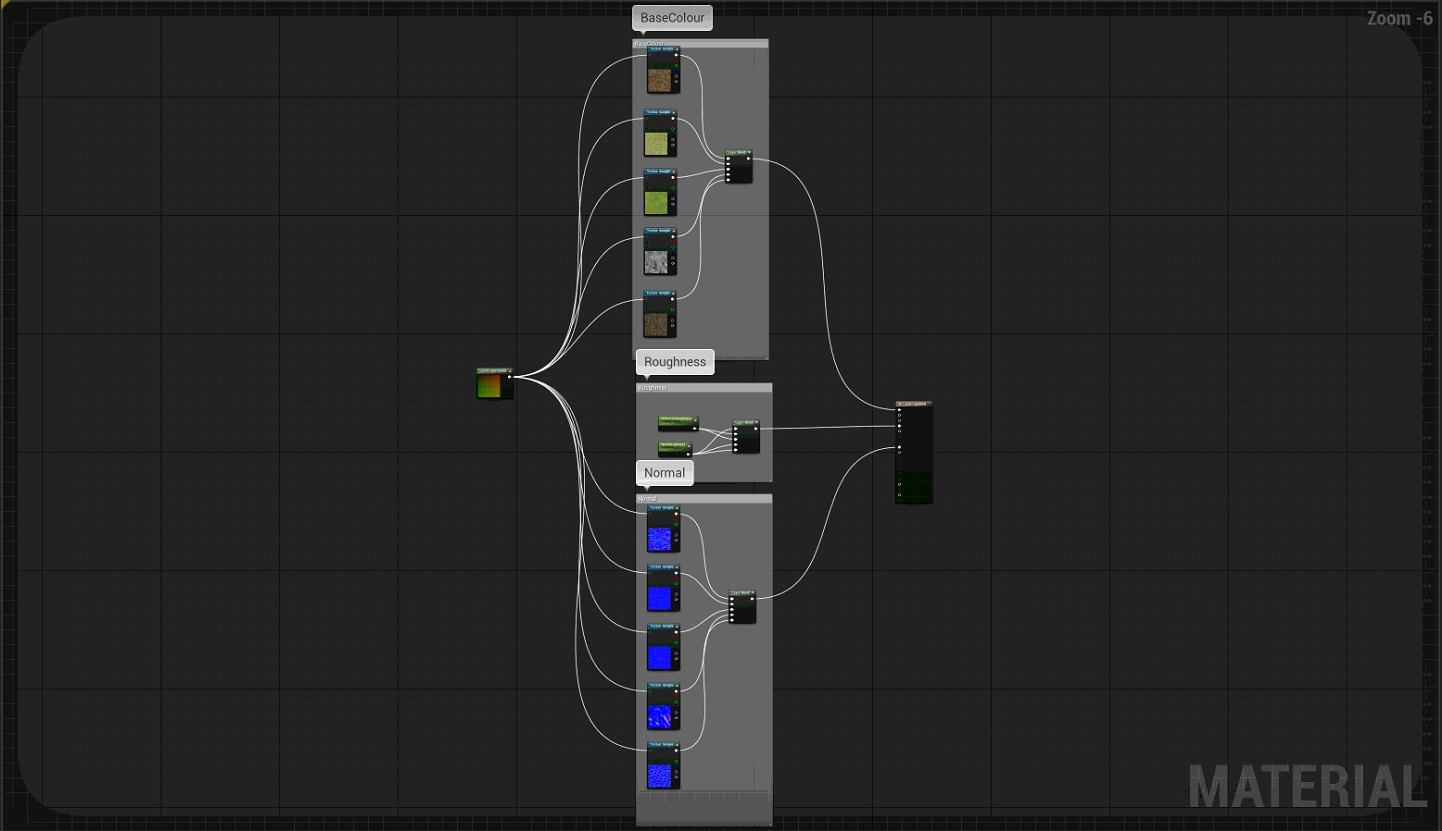
\includegraphics[width=16cm]{Landscape_Material.jpg}
	\caption{„Nudlový“ graf nového materiálu krajiny}
\end{figure}

Nově vytvořená a uložená, výše popsaná, síť materiálů byla nastavena jako materiál krajiny. Třetí nástroj funkce \textit{Landscape}, jak bylo uvedeno v předchozím textu, je malování (\textit{Paint}). Nástroje v režimu Malování umožňují upravovat vzhled krajiny pomocí selektivního nanášení vrstev materiálu na části krajiny.[43] Před samotným začátkem malování je nezbytné vytvořit pro každou vrstvu materiálu krajiny \textit{layer info object}. Existují dva druhy \textit{layer info object}: \textit{Weight-Blended} a \textit{Non Weight-Blended}. [43] Vlastnosti a podstata těchto informačních objektů jsou podrobně popsány v dokumentaci softwaru \textit{UE4} a z důvodu odlehlosti od tématu této práce nebudou dále popisovány. Pro jednotlivé vrstvy byl vytvořen \textit{layer info object} typu \textit{Weight-Blended}. Přes možnosti vrstvy pod názvem \textit{Layer Actions} byla celá krajina vykreslena funkcí \textit{Fill Layer} materiálem suché trávy (\textit{GrassDry}). Následně bylo prováděno ruční nanášení vrstev. \textit{UE4} umožňuje rozsáhlé nastavení kreslících nástrojů, pro krajinu v této práci byl použit pouze základní stětec se změnou parametrů intenzity nanášení (\textit{Tool Strength}), velikosti štětce (\textit{Brush Size}) a offsetu malování (\textit{Brush Falloff}). V oblastech pomyslných vyšších nadmořských výšek byla nanášena vrstva s materiálem kamene (\textit{Rock}), která postupně přes vrstvu hlíny (\textit{Dirt}) a lesní půdy (\textit{Forest}) přecházela v trávu. V oblastech s potenciální vyšší koncentrací vlhkosti byla nanesena vrstva bujné trávy (\textit{GrassLush}). Po vymalování krajiny byly upraveny parametry hrubosti materiálů a měřítko textur pro přirozený výsledný vzhled krajiny.

\begin{figure}[h!]
	\centering
	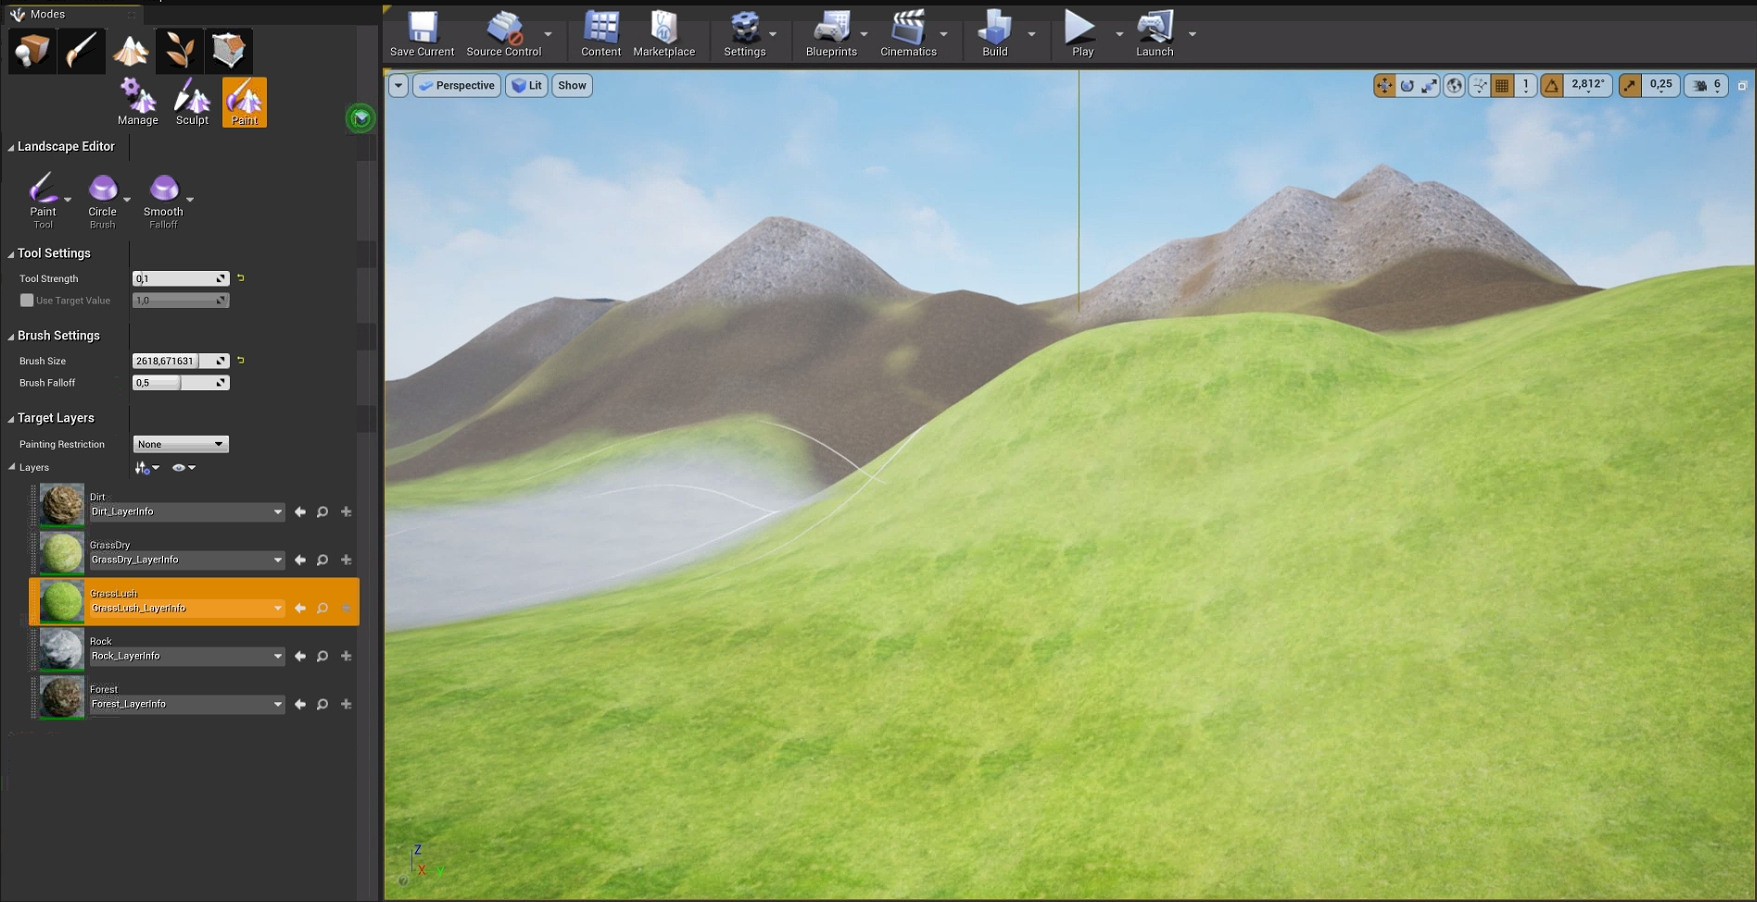
\includegraphics[width=16cm]{Landscape_Paint.jpg}
	\caption{Nanášení vrstev materiálu na krajinu}
\end{figure}

Následně byl importován a umístěn vytvořený model budovy muzea. Import lze provést pouhým přetažením \textit{FBX} souboru do požadované složky obsažené v projektu. Budova byla importována jako tzv. \textit{Static Mesh}. Software automaticky určí o jaký typ souboru se jedná a vyvolá dialogové okno s možnostmi nastavení importu. Veškeré možnosti a popis nastavení importu je také obsahem dokumentace \textit{UE4} a nebudou v této práci podrobně rozebírány. Importovaný soubor s modelem budovy neobsahoval kolize, které v \textit{UE4} slouží jako vymezení pevných (neprůchozích) částí objektů. Z tohoto důvodu byla při importu zvolena možnost automatického vygenerování kolize (\textit{Auto Generate Collision}). Veškeré ostatní možnosti byly ponechány na defaultní hodnotě. Po úspěšném importu následovalo přiřazování nových textur, které byly získány z volně dostupných zdrojů přímo v \textit{Epic Games - Marketplace}. Nové texturování jednotlivých elementů, vytvořených na základě prvotního přiřazení textur v softwaru SketchUp, bylo provedeno v \textit{UE4} editoru pro \textit{Static Mesh}. Po přiřazení textur všem částem budovy byla budova umístěna do krajiny. Problém nastal při testování průchodnosti budovy v režimu \textit{Play}. Uživateli nebyl umožněn průchod budovou, důvodem bylo špatné nastavení automaticky vygenerované kolizní sítě. Chyba byla vyřešena změnou výchozího typu kolize na \textit{UseComplexAsSimple}.\textit{ UseComplexAsSimple} znamená, že objekt přestane využívat jednoduchou kolizi. Ta neohraničuje pouze jednotlivá primitiva ze kterých je objekt složen, ale ohraničuje základními 3D tvary (krychle, koule apod.) objekt jako celek. Princip je podobný jako u obdélníku s minimální plochou, který je opsaný množině bodů, používaného při kartografické generalizaci. Volba \textit{UseComplexAsSimple} tedy použije kolizní síť složenou z jednotlivých elementů objektu a uživatel je poté omezen pouze fyzicky přítomnými prvky (zeď, schody, apod.).

\begin{figure}[h!]
	\centering
	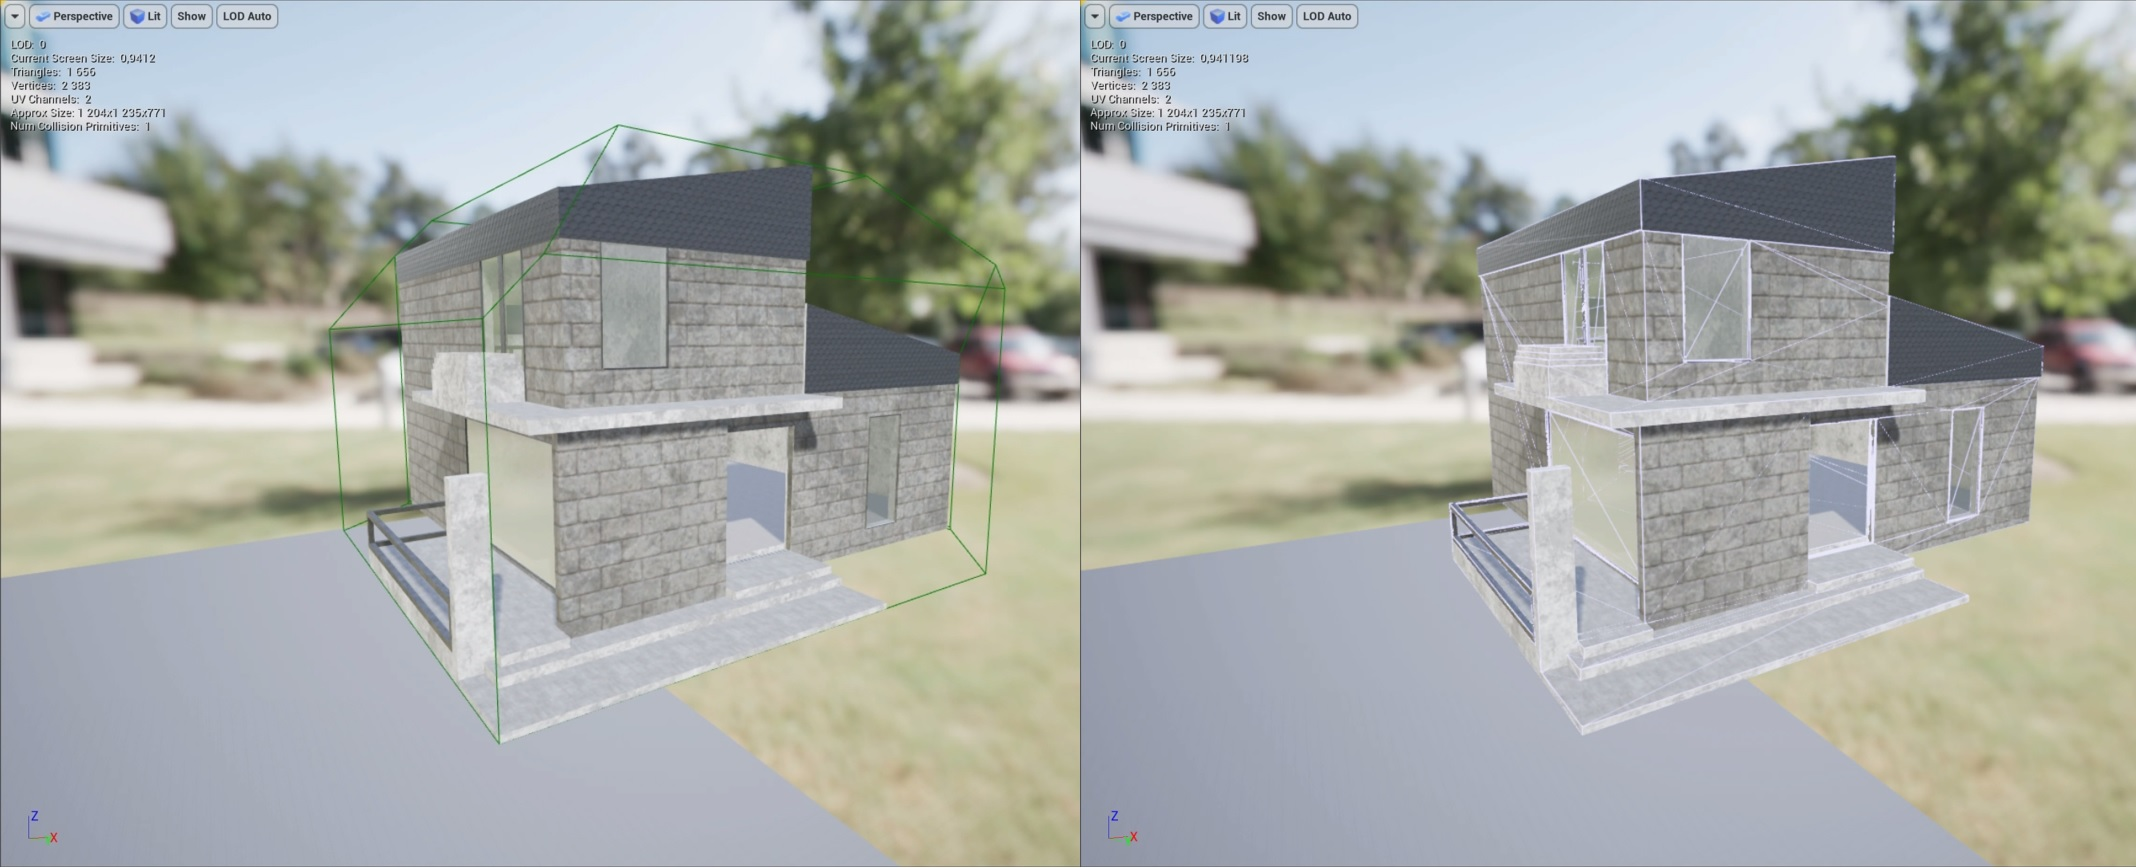
\includegraphics[width=16cm]{Collision.jpg}
	\caption{Vlevo je výchozí jednoduchá kolizní síť (zelené linie). Vpravo je kolizní síť komplexní (světlé linie). }
\end{figure}

\newpage
Jedním ze závěrečných kroků tvorby virtuálního prostředí bylo doplnění 3D prvků krajiny a vegetace. Pro tento krok byla využita funkce \textit{Foliage}. Tato funkce obsahuje nástroj \textit{Paint}, který umožňuje hromadné vkládání vybraných prvků do krajiny. Veškeré použité objekty byly do projektu přidány opět z volně dostupných zdrojů v \textit{Epic Games - Marketplace}. Jako první byly do funkce \textit{Foliage} importovány kameny. Celkem bylo použito 3 různých tvarů. Před začátkem kreslení bylo potřeba provést několik změn nastavení použitého nástroje. Nejprve byla snížena hodnota \textit{Pair Density}, jenž určuje hustotu rozmístění vybraných prvků. Následně byl také přizpůsoben rozměr vykreslované plochy tak, aby bylo možné docílit precizního umístění kamenů na plochu odpovídajícího materiálu krajiny. Jako filtr pro výběr elementů, na které budou kameny umisťovány, byla zvolena možnost \textit{Landscape}. Dalším krokem bylo nastavení parametrů jednotlivých objektů. Hustota umístění daného prvku do plochy odpovídající $1000 \times 1000$ jednotek (\textit{Density/1Kuu}) byla u všech tří typů nastavena na hodnotu 5. Další změna byla provedena v nastavení rozptylu měřítka jednotlivých kamenů. Rozptyl měřítka (\textit{Scale X}) byl nastaven na hodnotu od 0.5 do 1. Možnost zarovnání prvků na normálu (\textit{Align to Normal}) byla vypnuta. Těmito kroky bylo docíleno větší výsledné variace prvků v krajině. Veškeré ostatní možnosti byly ponechány na defaultní hodnotě. Pro provedení výše uvedeného nastavení byly hromadně umisťovány funkcí \textit{Paint} vybrané kameny. Po umístění kamenů byla obdobným způsobem vložena tráva.\\
\\
\textbf{Byly použity 3 typy trav, u kterých bylo provedeno následující nastavení:}\\
$Pair Density = 0.5 - 1; Filters = Landscape; Density/1Kuu = 5;$\\
$ Scale X: Min = 0.5, Max = 0.8; Align to Normal = off;$\\
ostatní hodnoty zůstaly nezměněny. \\
\\
\textbf{Přidávání stromů bylo provedeno s nastavením:} \\
$Pair Density = 0.2 - 1; Filters = Landscape;$ $Density/1Kuu = 1;$\\$
Scale X: Min = 0.7, Max = 1; Align to Normal = off;$\\
ostatní hodnoty zůstaly nezměněny. \\
\\
\textbf{Nastavení nástroje Paint pro křoviny:} \\
$Pair Density = 0.5 - 1; Filters = Landscape; Density/1Kuu = 10;$\\$
Scale X: Min = 0.4, Max = 0.6; Align to Normal = off;$\\  
ostatní hodnoty zůstaly nezměněny. \\
\\
\textbf{Jako poslední byla přidána luční flóra s nastavením:} \\
$Pair Density = 0.2 - 0.5; Filters = Landscape; Density/1Kuu = 5;$\\$
Scale X: Min = 0.5, Max = 1.5; Align to Normal = on;$\\
ostatní hodnoty zůstaly nezměněny. \\
V průběhu vykreslování byla některá nastavení upravována pro docílení co nejlepšího výsledku.\\
\\
Posledním krokem ve tvorbě virtuální krajiny a budovy muzea bylo vytvoření atmosféry a nastavení přírodního osvětlení. Volně dostupný materiál s názvem \textit{UE4 Lighting Presets 3 Pack} pro tvorbu denního osvětlení a atmosféry lze zdarma získat z internetového zdroje \textit{Gumroad.com} [59]. \textit{UE4 Lighting Presets 3 Pack} obsahuje tři složky s již vytvořenými prvky osvětlení, které je možné vložit přímo do vlastního projektu v \textit{UE4}. Samotné nahrání do projektu i dodatečné nastavení je obsahem video-návodu \textit{UNREAL ENGINE 4 LIGHTING TUTORIAL (UE4) - FREE DOWNLOAD LINK INCLUDED} dostupného na serveru $YouTube.com$ [58]. 

\begin{figure}[h!]
	\centering
	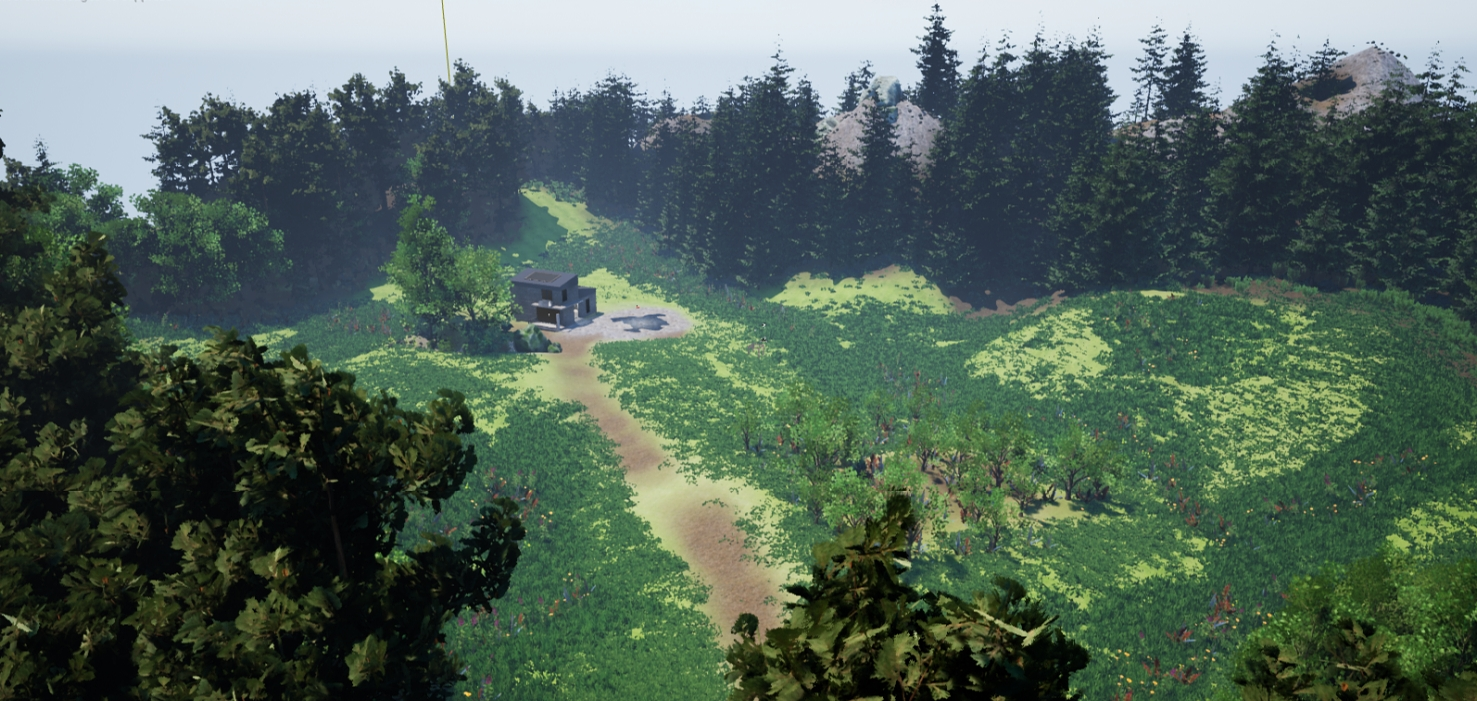
\includegraphics[width=16cm]{prostredi.jpg}
	\caption{Výsledný vzhled krajiny s budovou muzea}
\end{figure}

\chapter{Použitá data}
Dokumentace historických památek byla provedena bezkontaktní metodou, jejímž výstup-em jsou fotografie. Dokumentovány byly celkem čtyři objekty různých velikostí a povahy: dva římské sarkofágy (náhrobky), nacházející se v muzeu pod širým nebem v bývalém přístavu Caesarea v Izraeli, bronzová socha sv. Petra stojící v katedrále ve španělském Avile a chrámová stavba z hinduistické svatyně Pashupatinath v Kathmandu (Nepál).

\begin{figure}[h!]
	\centering
	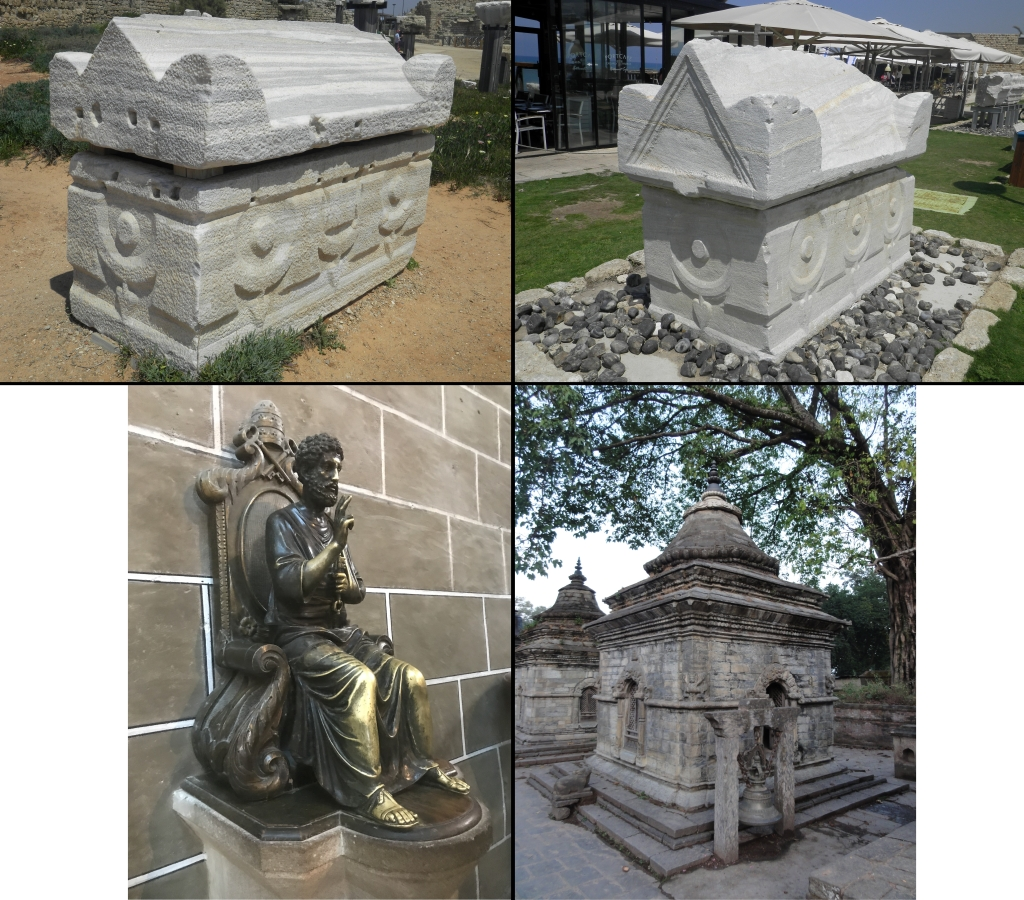
\includegraphics[width=14cm]{objekty.jpg}
	\caption{Fotografie dokumentovaných objektů}
\end{figure}


\section{Sběr dat}
Před samotnou tvorbou virtuálních modelů bylo nutné správně nafotografovat zájmové objekty. Při snímkování je vhodné zajistit neměnnost vnějších vlivů: stálé osvětlení, neměnná vzdálenost k objektu, nastavení fotoaparátu atd. Během fotografování by měla ohnisková vzdálenost objektivu zůstat konstantní. V praxi tento požadavek znamená vyloučení zoomování. Výše uvedené požadavky, vzhledem k následně použitému softwaru \textit{Agisoft Metashape}, není nutné striktně dodržovat. Současný software není určen pouze pro odborníky v oblasti fotogrammetrie, ale i pro širší veřejnost. Počet pořízených snímků se odvíjí od složitosti a rozměrů objektu. Pro kvalitní výsledný model je nutné provádět snímkování pravidelně z různých úrovní kolem celého objektu. Snímky by měly být konvergentní s velkým překrytem o hodnotě 70-80\%. Technologie \textit{image based modeling}, použitá v této práci, nevyžaduje odborné znalosti v oblasti fotogrammetrie. Důležité pro tuto metodu je dostatečné množství snímků s velkým překrytem z různých pozic vzhledem k zájmovému objektu. Část snímků by měla obsahovat i části, které jsou na jiných snímcích zakryté. [29]

\begin{figure}[h!]
	\centering
	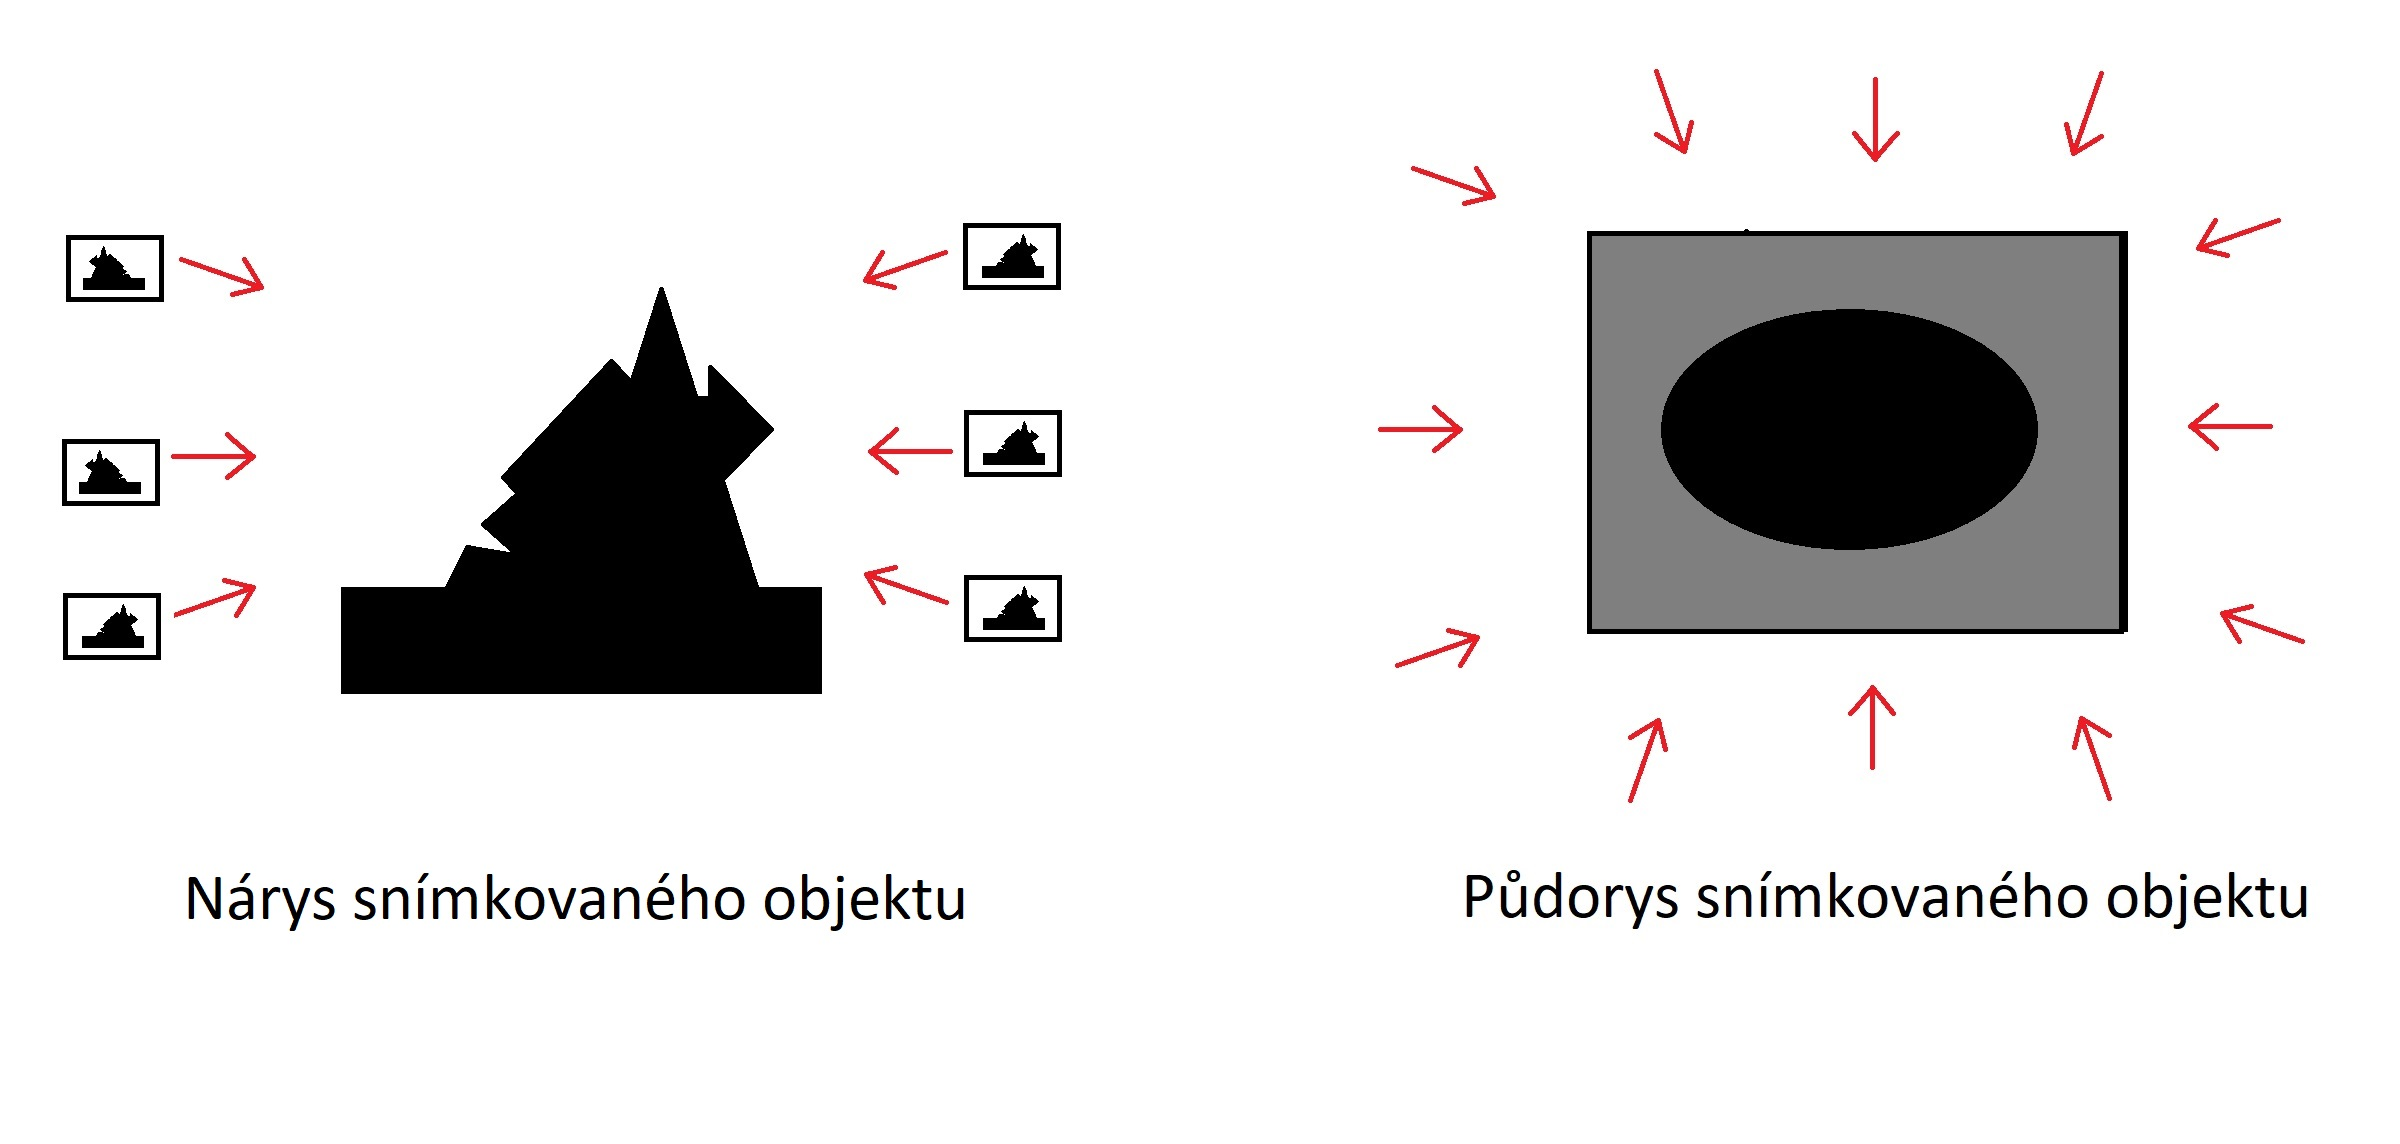
\includegraphics[width=16cm]{snímkování.jpg}
	\caption{Schéma vhodného rozložení os snímkování za účelem následného zpracování IBMR technologií}
\end{figure}

\subsection{Použité přístroje}
Snímky jednotlivých objektů byly pořízeny rozdílnými přístroji. Jednalo se celkem o dva běžné kompaktní fotoaparáty a jeden mobilní telefon. V současné době dovolují moderní technologie využití kamery chytrého telefonu pro účely dokumentace historických objektů, přičemž není problém dosáhnout obdobných výsledků jako při použití kompaktního fotoaparátu. Samozřejmě platí, že čím kvalitnější snímky jsou, tím bude kvalitnější i výsledný model objektu, a to především z hlediska šumu (nepřesně určené jednotlivé body). Zásadní pro kvalitu modelu je objektiv použitého zařízení. V současnosti disponují téměř všechna zařízení vybavená kamerou rozlišením vyšším, než je doporučená hodnota 6MPixelů. Důležitým faktorem je také ohnisková vzdálenost objektivu. U širokoúhlých objektivů je sice možné pořídit snímky s velkým překryvem, ale na úkor větší distorze. Ohnisková vzdálenost objektivu nesmí být ani příliš dlouhá, protože by znemožňovala pořízení snímků s dostatečným překryvem. [29]

\subsection*{Apple iPhone 7}
Socha sv. Petra byla dokumentována chytrým telefonem iPhone 7 od společnosti Apple. 

\begin{tabbing}
    Ohnisková vzdálenost: \=      
    \= 10 \kill
    \bfseries Parametry kamery \> \\[1mm]
    Model:	\>	iPhone 7\\
    Rozlišení:	\>	12 MPx\\
    Závěrka clony:	\>	f/1.8\\
    Ohnisková vzdálenost:	\>	4 mm\\
\end{tabbing}

\subsection*{Ricoh G700SE}
Dokumentace obou sarkofágů byla realizována kompaktním fotoaparátem Ricoh G700SE. Zařízení je vodotěsné a odolné proti pádu z výšky až 2 metry.  Fotoaparát má přesto dostatečnou kvalitu pro potřeby dokumentace. Uvedené jsou hodnoty pro oba objekty, přičemž první hodnota je pro Římský sarkofág 1, hodnota druhá pro Římský sarkofág 2. [44]

\begin{tabbing}
    Ohnisková vzdálenost: \=      
    \= 10 \kill
    \bfseries Parametry kamery \> \\[1mm]
    Model:	\>	G700 SE\\
    Rozlišení:	\>	12.10 MPx\\
    Závěrka clony:	\>	f/4.8; f/4.5\\
    Ohnisková vzdálenost:	\>	7 mm; 6 mm\\
\end{tabbing}

\subsection*{Sony DSC-HX5V}
Nejrozměrnější zpracovávaný objekt, chrámová stavba, byl snímkován kompaktním fotoaparátem od společnosti Sony s označením DSC-HX5V.

\begin{tabbing}
    Ohnisková vzdálenost: \=      
    \= 10 \kill
    \bfseries Parametry kamery \> \\[1mm]
    Model:	\>	DSC-HX5V\\
    Rozlišení:	\>	10.2 MPx\\
    Závěrka clony:	\>	f/3.5\\
    Ohnisková vzdálenost:	\>	4 mm\\
\end{tabbing}
Pořízení snímků pro dokumentaci nebylo předem plánované, vycházelo z okamžitého nápadu pokusit se vytvořit 3D model při návštěvě kulturních historických míst. Obecně snímkování trvalo od minut (sarkofágy) po cca 10-15 minut pro další objekty (sv.Petr a malý chrám).

\section{Zpracování dat}
Tvorba jednotlivých modelů z pořízených snímků probíhala v programu \textit{Agisoft Metashape Professional}. Tento software byl vyvinut společností Agisoft LLC. Společnost byla založena v roce 2006 a zabývá se technologiemi počítačového vidění. V současné době slouží software pro fotogrammetrické zpracování snímku. Hlavní oblastí využití je tvorba 3D dat pro práci v GIS společně s dokumentací kulturního dědictví. [45] Celý postup tvorby modelu s texturami vysoké kvality se skládá z pěti kroků: import dat, zorientování fotografií, tvorba hustého mračna bodů, tvorba trojúhelníkové sítě modelu a tvorba textury.

\subsection{Import}
Import fotografií lze provést přes ikonu \textit{Add Photos toolbar button} nebo přes možnost $Workflow \rightarrow Add Photos$ v horní části okna programu. Obě možnosti otevřou dialogové okno prohlížeče, ve kterém je možné vyhledat umístění a vybrat snímky určené pro tvorbu modelu. Snímky jsou importovány do složky \textit{Cameras} aktuálně vybraného \textit{Chunku}. Fotografie se zobrazí v okně \textit{Photos}, ale nejsou nahrány přímo do softwaru \textit{Metashape}, dokud nebudou skutečně zapotřebí. Po importu je možné snímky prohlížet i odstraňovat z aktuálního projektu. 

\begin{tabbing}
    Římský sarkofág 2:  \=      
    \= 10 \kill
    \bfseries Počet importovaných fotografií pro tvorbu modelů\> \\[1mm]
    sv. Petr:	\> 48\\
    Římský sarkofág 1:	\> 45\\
    Římský sarkofág 2:	\> 48\\
    Chrám:	\> 102\\
\end{tabbing}

\subsection{Aligning photos}
Po importu je potřeba vypočíst pozici a orientaci všech kamer, kterými byly fotografie pořízeny. Možnost \textit{Aligning photos}, která se po importu zpřístupní opět v sekci \textit{Workflow}, všechny fotografie porovná a zjistí, jak se v prostoru překrývají. Před samotným spuštěním procesu \textit{Aligning photos} je potřeba v dialogovém okně správně funkci nastavit. 

\begin{figure}[h!]
	\centering
	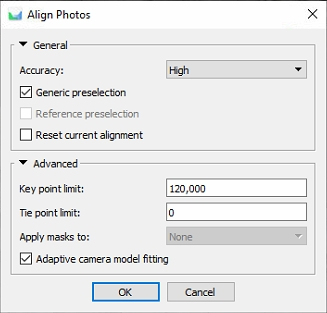
\includegraphics[width=5cm]{align.jpg}
	\caption{Dialogové okno pro nastavení \textit{Aligning photos}}
\end{figure}

\subsubsection*{Accuracy:} 
Nastavení, které určuje, jakou kvalitu fotografií má software pro výpočet použít. Pro tvorbu všech modelů v této práci byla zvolena možnost \textit{High}, při které vstupují fotografie do výpočtu v plném rozlišení.

\subsubsection*{Pair Preselection:} Možnost, která je vhodná pro snížení časové náročnosti výpočtu při zpracování velkého množství vstupujících fotografií. Tato takzvaná předvolba dvojice vytváří podmnožiny párů obrazových dat, které mají být následně porovnány. V programu \textit{Agisoft Metashape} jsou k dispozici dvě možnosti: \\
1) Generic preselection - Odpovídající fotografie jsou nejprve párovány na základě nižší přesnosti. \\
2) Reference preselection - Fotografie jsou vybírány na základě naměřeného umístění kamery, pokud je k dispozici. Šikmé snímky musí obsahovat hodnotu výšky ve stejném souřadnicovém systému, jako jsou souřadnice kamer. \\
Pro výpočet orientace kamer všech objektů v této práci byla zvolena pouze první možnost (\textit{Generic preselection}) z důvodu, že souřadnice kamer ani nadmořských výšek nebyly známy. 

\subsubsection*{Key point limit:}
Hodnota udává horní hranici počtu bodů, které z každého snímku vstupují do výpočetní funkce v aktuální fázi zpracování. Pokud je hodnota 0, pak je programu umožněno nalézt maximální počet vstupních bodů. Rizikem takového nastavení je vysoký počet nespolehlivých bodů. Pro tvorbů modelů byla nastavena mezní hodnota maximálně na 120,000. 

\subsubsection*{Tie point limit:}
Limit, který také umožňuje redukci počtu bodů vstupujících do výpočetních funkcí. Toto omezení způsobí, že z vybraných bodů, které byly v předchozím kroku omezeny horní hodnotou \textit{Key point limit}, vybere software pouze zadaný počet těch nejkvalitnějších. Při zadání hodnoty 0, není tento krok proveden. Hodnota 0 byla zadána při tvorbě všech objektů, vyjma Římského sarkofágu 1, u kterého byla zadána hodnota 4,000.

\subsubsection*{Adaptive camera model fitting:} 
Tato možnost provede automatický výběr parametrů kamery, které budou zahrnuty do výpočtu na základě odhadu jejich spolehlivosti.\\
\\
Po provedení procesu \textit{Aligning photos} se v grafickém okně zobrazí řídké mračno bodů vytvořené na základě výpočtu orientace a polohy snímků. V okně obsahujícím importované fotografie je nutné zkontrolovat, které fotografie nebyly použity. Jestliže nepoužité fotografie je potřeba zařadit do projektu, musí být uměle připojeny prostřednictvím identických bodů obsažených na jiných zařazených fotografiích. Druhou možností, která byla použita pro projekt chrámové stavby, konkrétně pro připojení její vnitřní části, je samostatná tvorba jednotlivých částí v oddělených \textit{chunks}, ty jsou v závěrečné fázi tvorby modelu spojeny. 

\subsection{Build dense cloud}
Po tvorbě a dodatečných úpravách řídkého mračna bodů bylo generováno mračno bodů husté. Husté mračno bodů vytvořené programem \textit{Metashape} ze zorientovaných snímků je velmi podobné mračnům bodů získaných metodou laserového skenování. Na základě odhadu pozice kamery vypočítá software hloubkové informace bodů každého snímku a následně je sloučí do jednoho mračna. Tvorba hustého bodového mračna se skládá ze čtyř částí:\\
1) Kontrola a úprava prostorového ohraničení, ve kterém bude výpočet a tvorba probíhat. \\
2) Výběr příkazu \textit{Build Dense Cloud} z nabídky \textit{Workflow}.\\
3) Zadání parametrů pro tvorbu hustého mračna v dialogovém okně. \\
4) Zpracování dat a tvorba hustého mračna bodů softwarem. \\
Nastavované parametry zadávané v části 3) ovlivňují kvalitu výsledného mračna, dobu procesu tvorby i způsob, jakým budou algoritmy body vyhodnocovat. 

\subsubsection*{Quality:}
Parametr, který určuje podrobnost a přesnost výsledku operace. Vyšší kvalita znamená také vyšší časovou náročnost generování mračna bodů. Princip je obdobný jako u výše uvedeného parametru \textit{Accuracy} v \textit{Photo Alignment}. Pro tvorbu modelů v této práci byla vždy nastavena možnost \textit{High}, která zaručuje plnou kvalitu snímků pro vstup do výpočtů.

\subsubsection*{Depth filtering modes:}
Při tvorbě hustého mračna počítá \textit{Metashape} hloubkovou mapu každého snímku. Z důvodu špatné kvality snímků mohou být některé hodnoty značně odlehlé. Proto je důležité  nastavit správný režim filtrace vzhledem k povaze projektu. Pokud zpracovávaný objekt obsahuje drobné detaily, které je třeba ve výsledném modelu zachovat, pak je vhodná volba režimu \textit{Mild}. Režim \textit{Aggressive depth filtering} je určen pro projekty, které neobsahují smysluplné drobné detaily. Tato možnost je vhodná především pro zpracování leteckých dat. Třetí možnost, \textit{Moderate}, je pomyslným středem mezi oběma výše uvedenými režimy. S nastavením filtrace je vhodné, pro docílení požadovaných výsledků, experimentovat. Objekty zpracovávané v této práci vždy obsahovaly drobné detaily. Experimentálním testováním byla vyhodnocena možnost \textit{Mild} jako nejvhodnější pro tento typ dat. 

\subsubsection*{Calculate point colors:}
Umožňuje vypnutí obarvování bodů. Tato možnost byla vždy aktivní vzhledem k povaze projektu.\\
\\
Po vytvoření hustého mračna bodů bylo provedeno ořezání dat tak, aby pro následující zpracování obsahovala co nejméně odlehlých nebo nevhodných bodů. 

\subsection{Build mesh}
Předposledním krokem bylo vytvoření síťového modelu složeného z trojúhelníků na základě hustého mračna bodů. Postup byl následující:\\
1) Kontrola a případná úprava prostorového ohraničení dat vstupujících do výpočtu. \\
2) Spuštění příkazu \textit{Build Mesh} lze opět provést z nabídky \textit{Workflow}.\\
3) Spuštění příkazu vyvolá dialogové okno, kde je možné zadat parametry nastavení tvorby modelu. \\
4) Po správném nastavení byla spuštěna automatická tvorba síťového modelu. \\
Možnosti volby metod a změny nastavení pro následnou automatickou tvorbu modelu umožňují uživateli dosáhnout optimálních výsledků s ohledem na typ vstupních dat.

\subsubsection*{Source data:}
Nastavení, které určuje zdroj dat vstupujících do výpočtu tvorby síťového modelu. V této práci byly generovány modely pouze na základě vstupu hustého mračna bodů, tedy možnosti \textit{Dense cloud}.

\subsubsection*{Surface type:}
Tato volba skýtá dvě možnosti nastavení typu tvorby modelu: \textit{Arbitrary} a \textit{Height field}. \\
První uvedenou volbu \textit{Arbitrary} je možné použít pro tvorbu libovolného modelu. Metoda nevytváří žádně předpoklady týkající se typu výsledného modelu. Z obou variant je tato možnost z hlediska výpočetní paměti náročnější. Pro tvorbu objektů virtuálního muzea byla volena výhradně tato možnost.\\
Druhá volba \textit{Height field} je 2.5 dimenzionální metoda zpracování, která optimalizuje tvorbu pro rovinné povrchy. Tato možnost je vhodná pro zpracování leteckých snímků a velkých datových sad. 

\subsubsection*{Quality:}
Určuje požadovanou kvalitu tvorby modelu z hloubkových map za předpokladu, že jsou vybrány jako zdroj.

\subsubsection*{Face count:}
Nastavení \textit{Face count} specifikuje maximální počet polygonů tvořící výsledný síťový model. Přednastavené hodnoty (\textit{High, Medium, Low}) představují optimální počet polygonů sítě pro odpovídající kvalitu výsledného modelu. Hodnotu lze nastavit také přímo, zadáním konkrétního čísla horní hranice počtu polygonů. Parametr byl u všech modelů nastaven na hodnotu \textit{High}.
 
\subsubsection*{Interpolation:}
Tvorbu modelu lze provést s možností interpolace v oblastech neobsahujících data. Interpolaci je možné provést v jednom ze tří režimů: vypnutá, povolená základní a povolná extrapolace. Pokud je interpolace vypnuta, vede tvorba sítě k výsledkům, shodujících se s hustým mračnem bodů na vstupu. Tato možnost, na základě experimentálně dosažených výsledků, nebyla volena pro žádný objekt. Výchozí možnost povolující interpolaci vyplňuje určité oblasti bez dat, nacházejících se v kruhu o určitém poloměru. Tato volba nezaručuje kompletní zacelení modelu. Interpolace byla využita, opět na základě experimentálně získaných zkušeností, u většiny zpracovávaných objektů. Režim extrapolace generuje model bez děr, které jsou zaceleny metodou extrapolace. Tato metoda umožňuje vytvářet velké neexistující plochy za účelem doplnění modelu, ty ale mohou být v následném zpracování snadno odstraněny. Extrapolace byla použita u modelu \textit{Římského sarkofágu 1}, a to především z důvodu prezentace využitelnosti různých možností nastavení.

\subsubsection*{Point classes:}
Nastavení volby třídy bodů, vstupujících do výpočtu, je určeno pro projekty obsahující klasifikovaná mračna bodů. V této práci nebyla klasifikace provedena.

\subsubsection*{Calculate vertex colors:}
Pokud zdrojová data obsahují informace o barvách bodů, lze prostřednictvím této možnosti přiřadit barvy vrcholům sítě. Jak je uvedeno v předchozím kroku, zpracovávaná mračna bodů obarvena byla. Proto byla tato možnost využita u všech modelů. 

\subsubsection*{Use strict volumetric masking:}
Tato možnost je určena pro projekty obsahující masky fotografií, které nebyly součástí této práce.

\subsubsection*{Reuse depth maps:}
Volba umožňující opětovné použití hloubkových map. Metoda je dostupná pouze pro tvorbu na základě hloubkových map, která nebyla součástí této práce.

\subsection{Build texture}
Závěrečným krokem tvorby virtuálních modelů bylo vytvoření textury. Pro generování textury aktuálního objektu je ve \textit{Workflow} menu možnost \textit{Build Texture}. Po nastavení níže uvedených parametrů tvorby je textura automaticky vygenerována a umístěna na model. 

\subsubsection*{Mapping mode:}
Způsob mapování určuje, jakým způsobem bude objekt do textury zabalen, z více možností, které jsou popsány v návodu pro Agisoft Metashape Pro, byla u všech modelů volena možnost \textit{Generic}. Jedná se o výchozí režim generického mapování, jenž umožňuje parametrizovat textury pro libovolné geometrie. Nejsou zde obsaženy žádné předpoklady týkající se typu dat, která mají být zpracována. 

\subsubsection*{Blending mode:}
Volba způsobu, jakým budou výsledné textury kombinovat hodnoty pixelů ze zpracovávaných fotografií. Metashape nabízí celkem pět možností: \textit{Mosaic, Average, Max Intensity, Min Intensity a Disabled}.\\
Možnost \textit{Mosaic} má implementovaný dvoufázový přístup. Metoda provádí míchání \\nízkofrekvenční složky dat pro překryv snímků za účelem potlačení viditelnosti švu na textuře. Druhou složkou jsou data s nejvyšší frekvencí, která zajišťují detaily obrazu. Ta jsou převzata pouze z jednoho zdroje s nejlepší kvalitou v zájmové oblasti. \\
\textit{Average} používá vážený průměr hodnoty všech pixelů z jednotlivých fotografií. Váha je určena stejným parametrem, kterým jsou určovány také vysokofrekvenční složky v režimu \textit{Mosaic}. \\
Metoda \textit{Max Intensity} použije fotografii, která má maximální intenzitu odpovídajícího pixelu.\\
Metoda \textit{Min Intensity} použije fotografii, která má minimální intenzitu odpovídajícího pixelu.\\
Poslední možnost \textit{Disabled} vypne kombinování hodnot pixelů a pro tvorbu textury použije fotografie s nejvyšší frekvenční složkou dat. \\
Na základě testování, spočívajícího v tvorbě textur různými metodami kombinace hodnot pixelů, byla pro veškeré textury vytvářené v této práci zvolena možnost mozaikování.

\subsubsection*{Texture size/count:}
Hodnota určuje rozlišení textury v pixelech a počet souborů pro její export. Vícesouborové exportování textur umožňuje vyšší rozlišení výsledné textury modelu. Vzhledem k velikosti zpracovávaných objektů nebylo potřebné vytvářet více souborů pro export textur. 

\subsubsection*{Enable ghosting filter:}
Tato možnost nastavení pro generování textur zabraňuje tzv. \textit{ghosting effect}. V praxi to znamená, že pokud fotografie obsahují například pohybující se rozmazané objekty, které nebylo možné zkonstruovat, jsou obrazová data objektů na textuře potlačena. Tato volba byla při tvorbě všech modelů aktivována.\\
\\
Výsledné virtuální modely historických objektů byly exportovány do formátu \textit{OBJ}. Software automaticky provádí také export textur do souboru ve formátu \textit{JPEG}. Kompletní hodnoty a nastavení, použité při tvorbě modelu v jednotlivých výše popsaných krocích, jsou obsahem přílohy.

\chapter{Příprava modelů pro vizualizaci ve VR}
Před samotným umístěním modelů, vzniklých výše uvedeným způsobem, do virtuálního prostředí, bylo nutné provést úpravy, které zajistí bezproblémovou vizualizaci. Úpravy byly prováděny především s ohledem na výpočetní výkon PC a zachování potřebné kvality detailů objektů. 

\section{Retopologie modelů}
Vizualizace síťového modelu vysoké kvality (počet trojúhelníků v řádech stovek tisíc), tzv. \textit{High-poly} modelu, je náročná na výpočetní výkon i úložný prostor zařízení. Například model sochy sv. Petra měl po exportu do formátu \textit{OBJ} velikost přibližně \textit{166 MB}. Ve vyšším počtu jsou soubory obdobné velikosti obtížně přenositelné i prezentovatelné. Bylo tedy nutné provést decimaci trojúhelníkové sítě jednotlivých objektů (retopologii) a vytvořit tak tzv. \textit{Low-poly} modely. Decimace modelů byla v této práci provedena dvěma způsoby: v aplikaci \textit{Instant Meshes} a přímo v softwaru \textit{Agisoft Metashape}.

\subsection{Instant Meshes}
\textit{Instant Meshes} je volně dostupný program pro automatickou retopologii síťových modelů. Software je založen na článku \textit{Instant Field Aligned Meshes} skupiny pod názvem \textit{Interactive Geometry Lab}, vedené profesorkou Olgou Sorkine-Hornung, který byl představen na konferenci \textit{Siggraph Asia} v listopadu 2015. Hlavním autorem je Wenzel Jakob. Software převede importovanou geometrii na pravidelnou čtyřúhelníkovou nebo trojúhelníkovou síť, automaticky vyhodnotí zakřivení geometrie a generuje hrany s ohledem na tvarově ostré prvky modelu. Software dokáže zpracovat data v podobě mračen bodů z 3D skenerů a je schopen pracovat s velmi velkými množinami. Video prezentující software ukazuje převod sítě složené z 372 milionů trojúhelníků na čtvercovou, s přibližně 100000 vrcholy, za méně než 10 minut (dostupné na serveru \textit{YouTube.com}[58]). Retopologizovaná geometrie může být exportována do souboru ve formátu OBJ.[2]\\
\\
Nejprve byl zájmový \textit{High-poly} model naimportován do softwaru prostřednictvím tlačítka \textit{Open mesh}. Následně byla nastavena možnost \textit{Remesh as} na \textit{triangles}. Hodnota \textit{Target vertex count} udávající horní hranici počtu vrcholů, nově vznikajícího decimovaného modelu, byla nastavena prostřednictvím posuvníku na hodnotu 23.15 K. Následně byl proveden výpočet \textit{N-RoSy} pole prostřednictvím implementované funkce \textit{Orientation field}. Funkce z množiny směrů, získaných z povrchu importovaného modelu, určí hrany, ke kterým bude výsledný model vyrovnáván. Druhým nutným výpočtem je \textit{Position field}. Tento krok vypočítal lokální, \textit{per-vertex} (u;v), parametrizaci. Hodnoty souřadnic v podobě celého čísla v této parametrizaci odpovídají vrcholům výsledné sítě a gradient je přesně zarovnán s vypočteným orientačním polem z kroku předchozího. Po úspěšném provedení výše uvedených výpočtů byla provedena extrakce sítě \textit{Low-poly} modelu a následné uložení do souboru ve formátu \textit{OBJ}.

\begin{figure}[h!]
	\centering
	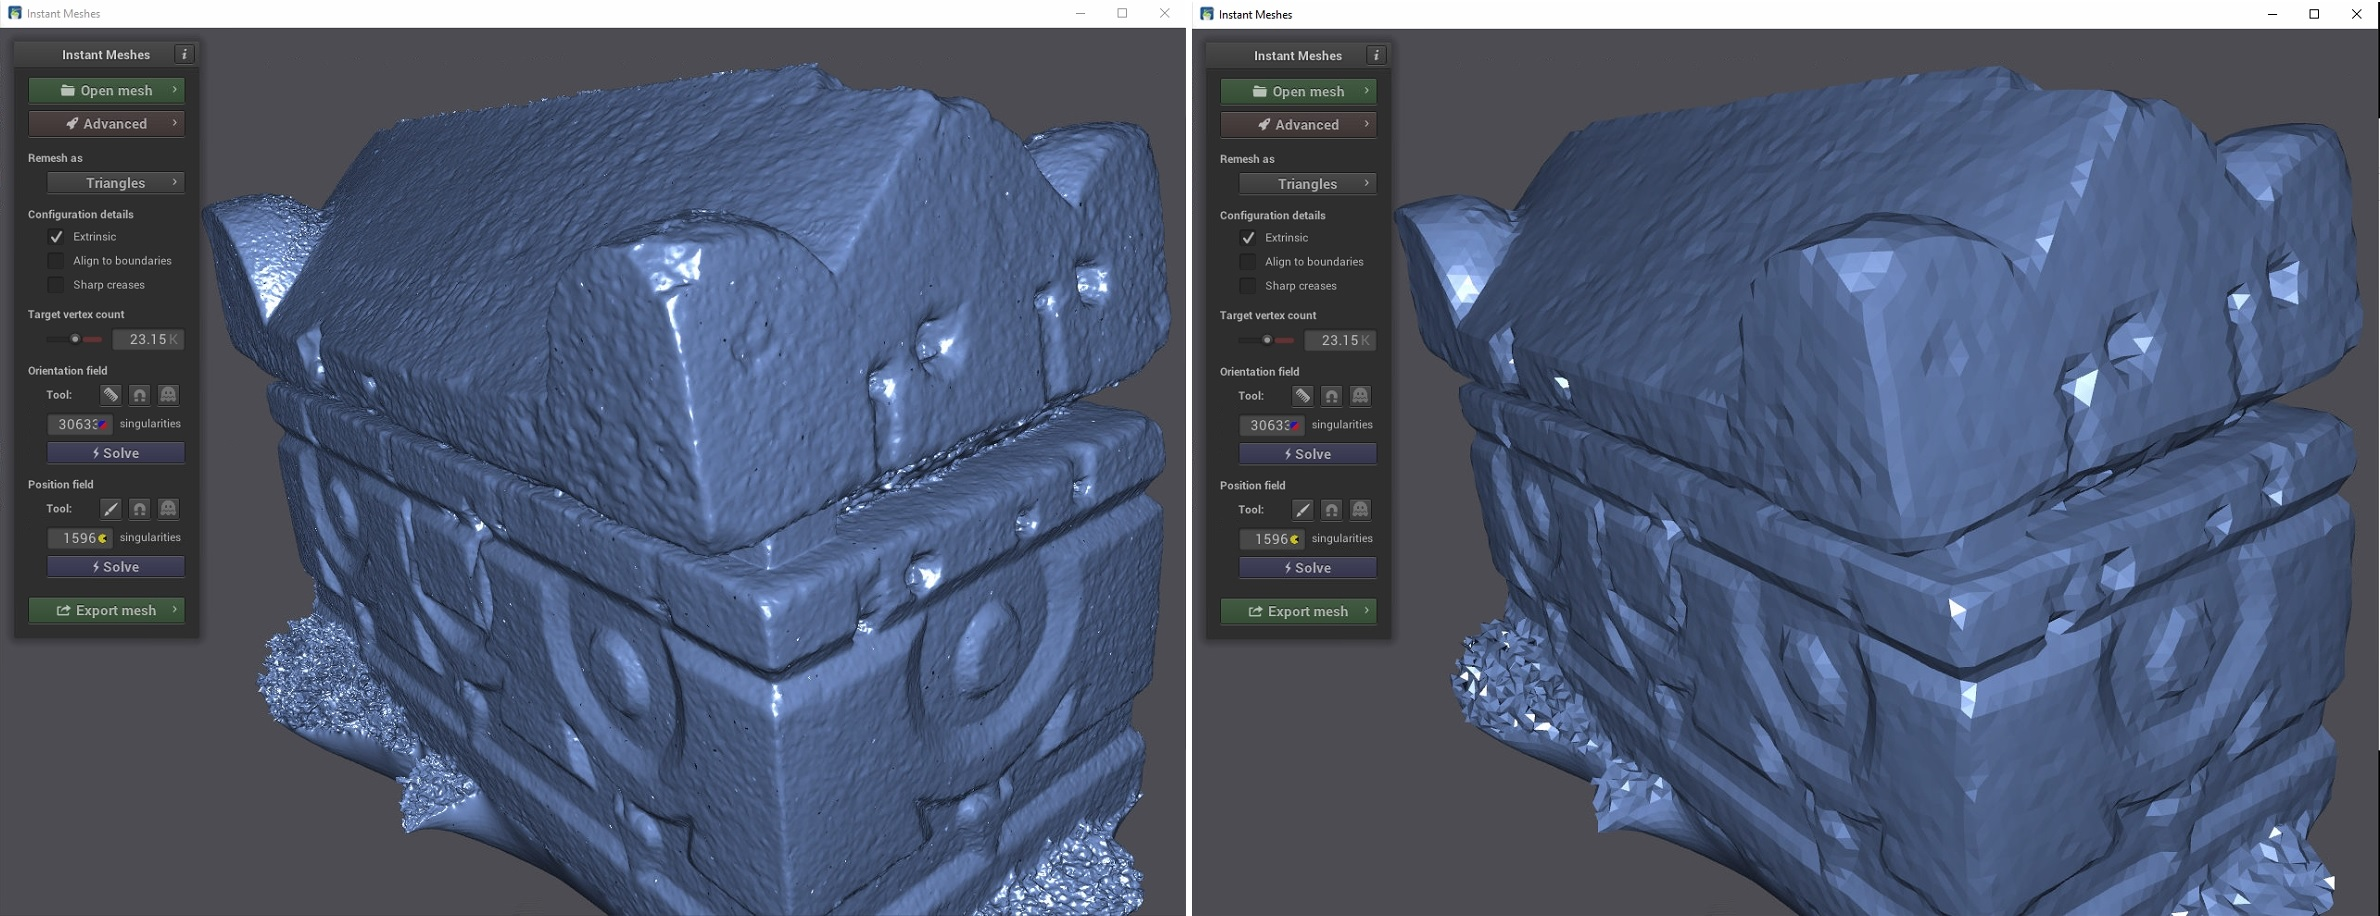
\includegraphics[width=16cm]{IM.jpg}
	\caption{Příklad retopologie modelu Římského sarkofágu 1 v softwaru \textit{Instant Meshes}: vlevo je původní \textit{High-poly} model, který je složen z 3048821 trojúhelníků (hodnota \textit{faces}); vpravo je výsledný \textit{Low-poly} model obsahující pouze 43490 trojúhelníků}
\end{figure}

\subsection{Agisoft Metashape}
Druhý způsob provedení retopologie modelu spočíval v opětovné tvorbě síťového modelu v softwaru \textit{Agisoft Metashape}. Původní projekt, který vznikl při tvorbě \textit{High-poly} modelu, byl uložen pod novým názvem a následně v programu otevřen. Z výše uvedených kroků, pro vytvoření síťového modelu objektu, bylo nutné opětovně provést krok \textit{Build mesh}. Na rozdíl od nastavení parametrů tvorby \textit{High-poly} modelu byla v tomto případě nastavena hodnota \textit{Face count} na řádově nižší číslo. \\

\begin{tabbing}
    Římský sarkofág 2: \=      
    \= 10 \kill
    \bfseries Zadané hodnoty \textit{Face count} pro tvorbu Lo-poly modelů\> \\[1mm]
    sv. Petr:	\>	30 000\\
    Římský sarkofág 1:	\>	provedeno v softwaru \textit{Instant Meshes}\\
    Římský sarkofág 2:	\>	30 000\\
    Chrám:	\>	80 000\\
\end{tabbing}

\newpage
\begin{tabbing}
    Římský sarkofág 2: \=  High-poly: 1110875; \= Low-poly: 30150      
    \= 10 \kill
    \bfseries Skutečná hodnota \textit{Face count} pro jednotlivé modely\> \\[1mm]
    sv. Petr:	        \> \textit{High-poly}: 1110875;\> \textit{Low-poly}: 30150 \\
    Římský sarkofág 1:	\> \textit{High-poly}: 3048821;\> \textit{Low-poly}: 43490 \\
    Římský sarkofág 2:	\> \textit{High-poly}:  438122;\> \textit{Low-poly}: 24932 \\
    Chrám:	            \> \textit{High-poly}: 5183028;\> \textit{Low-poly}: 78652 \\
\end{tabbing}
Po výše uvedeném nastavení byl proveden opětovný výpočet a tvorba modelu. Výsledný model je složen z přibližně stejného počtu trojúhelníků, jako je hodnota, která byla zadána do kolonky parametru \textit{Face count}. Na závěr byl proveden export nově vzniklého \textit{Low-poly} modelu. 

\begin{figure}[h!]
	\centering
	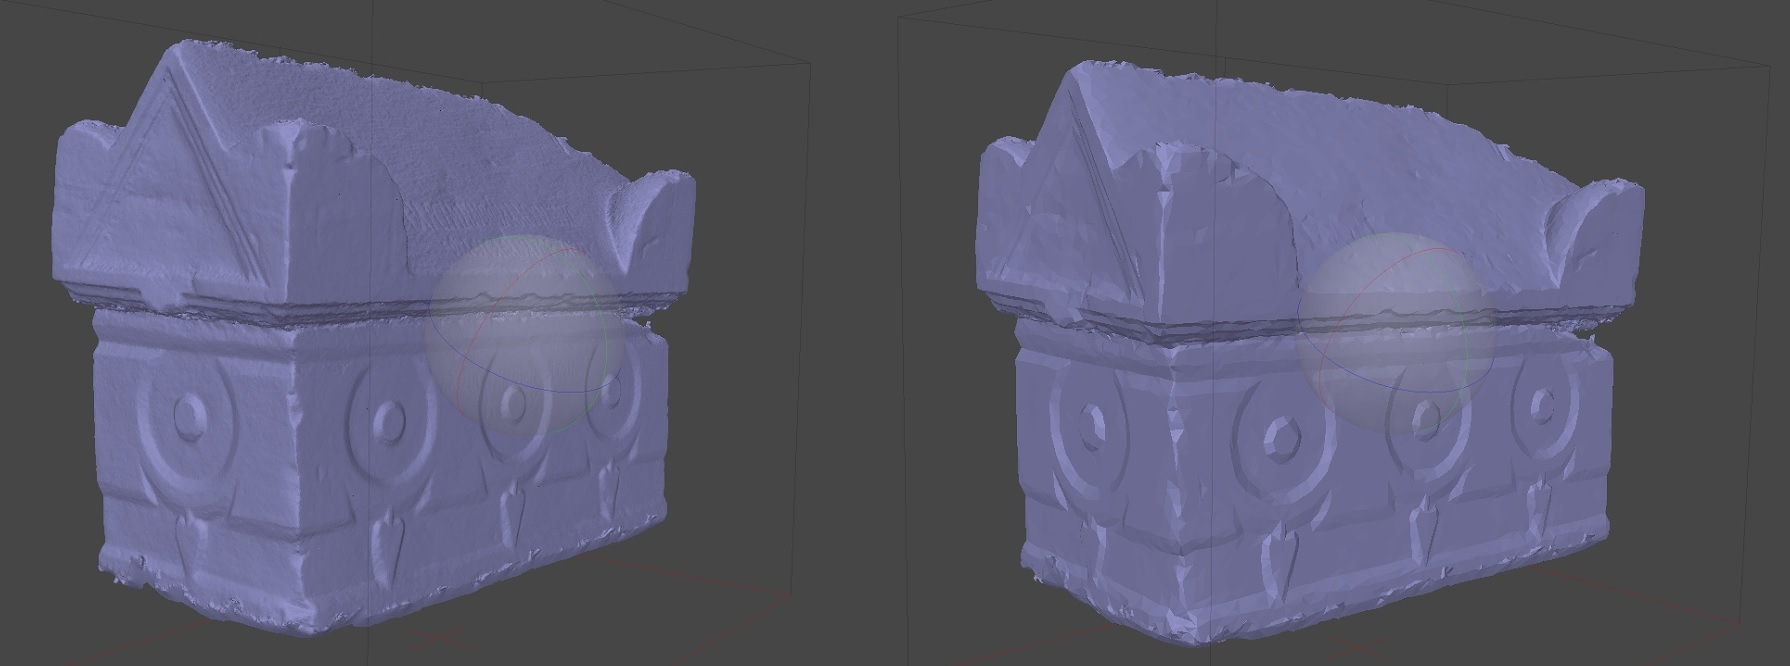
\includegraphics[width=16cm]{retopologie_agisoft.jpg}
	\caption{Příklad retopologie modelu Římského sarkofágu 2 v softwaru \textit{Agisoft Metashape}: vlevo je původní \textit{High-poly} model; vpravo je výsledný \textit{Low-poly} model}
\end{figure}

\section{Tvorba normálových map}
Retopologie sice sníží velikost výsledného modelu z desítek až stovek MB na jednotky, ale zároveň snižuje také kvalitu detailů povrchu. Pro věrnou vizualizaci bylo potřeba provést tzv. vypečení textury z \textit{High-poly} modelu na odpovídající \textit{Low-poly} model. Jednalo se o vytvoření normálové mapy textury, která při následné vizualizaci vytváří iluzi nerovnosti povrchu bez existence její geometrie. Normálové mapy textur ovlivňují výpočet osvětlení plochy. Vypečení textury bylo provedeno ve volně dostupném softwaru \textit{xNormal}. \\
Proces tvorby normálové mapy se skládá z pěti kroků:\\
1) High definition meshes - volba \textit{High-poly} modelu, ze kterého bude textura napečena. \\
2) Low definition meshes - volba \textit{Low-poly} odpovídajícího modelu, na který bude textura napečena.\\
3) Baking options - nastavení exportu a vlastností nově vznikajících map.\\
4) Ray distance calculator
5) Generate maps - vytvoření normálové mapy.\\
\\
Pro každý model v této práci byl proveden stejný postup, složený z výše uvedených kroků. Vytvořené normálové mapy textur jednotlivých objektů byly uloženy do souboru ve formátu JPEG a použity pro následnou tvorbu materiálů v \textit{UE4}. 

\begin{figure}[h!]
	\centering
	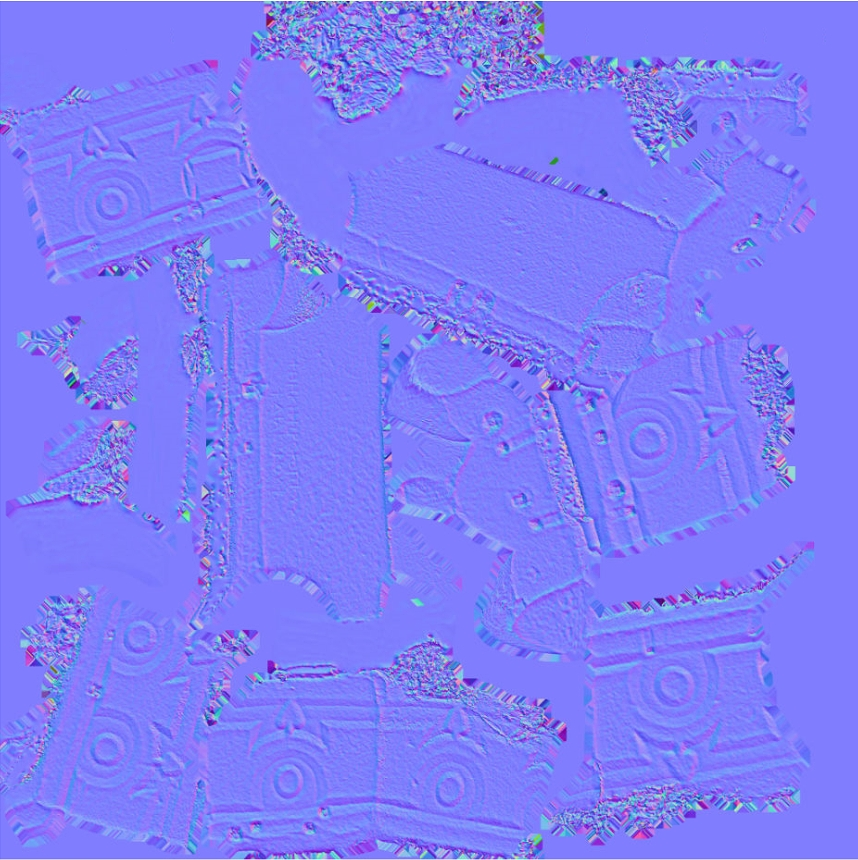
\includegraphics[width=9cm]{normal_maps.jpg}
	\caption{Normálová mapa textury Římského sarkofágu 2}
\end{figure}

\section{Unwrapping textur}
Textury modelů existují pouze ve 2D prostoru. Pro vytvoření mapy textury slouží souřadn-ice \textit{U} a \textit{V}, které reprezentují hodnoty na vodorovné a svislé ose textury. UV mapování je proces, který převede 3D polygonovou síť na 2D informaci tak, že pak lze kolem modelu texturu "omotat". Pro optimální výkon softwaru, ve kterém bude model vizualizován, je vhodné textury přetvořit, neboli provést tzv. \textit{unwrap UV}. Rozbalení UV si lze představit jako obrácený postup skládání krychle z papíru. Na modelu jsou definovány švy, podle kterých bude síť rozložena do roviny. Bodům takto vzniklé plochy jsou následně přiřazeny právě souřadnice U a V. Teto proces je značně časově náročný a nebyl v této práci prováděn, ačkoliv by z hlediska optimalizace pro herní engine byl vhodný. 

\begin{figure}[h!]
	\centering
	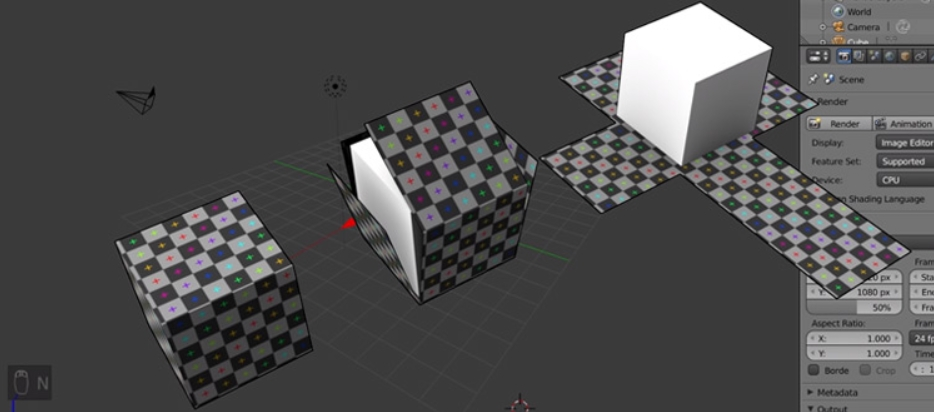
\includegraphics[width=14cm]{wrapping.jpg}
	\caption{Princip rozbalování textury (unwrapping)}
\end{figure}

\chapter{Import a vizualizace historických objektů ve VR}
Pro možnost umístění připravených modelů do virtuálního muzea bylo nutné provést import dat do projektu v \textit{UE4} a následně vytvořit nové materiály pro jednotlivé objekty. 

\section{Import modelů do UE4}
Import modelů do projektu byl proveden obdobným způsobem jako import budovy muzea. Soubory ve formátu \textit{OBJ} byly importovány do příslušné složky s názvem \textit{Geometry} pouhým přetažením. V dialogovém okně, pro nastavení parametrů importu, byla opět zvolena možnost automatické tvorby kolizní sítě. Veškeré ostatní hodnoty zůstaly nezměněné. 

\begin{figure}[h!]
	\centering
	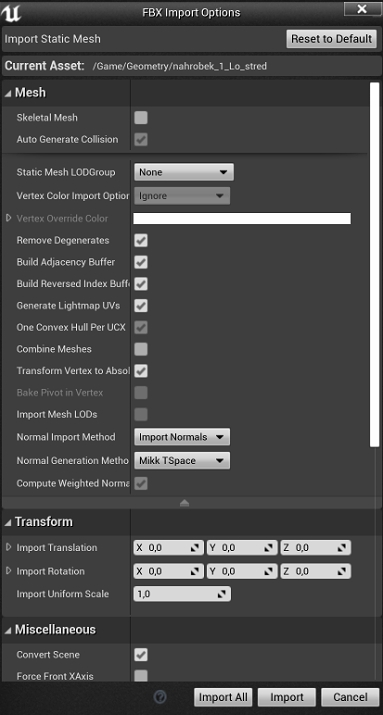
\includegraphics[width=5cm]{import_UE.jpg}
	\caption{Dialogové okno pro nastavení parametrů importu}
\end{figure}

\section{Tvorba a přiřazení materiálů}
Před začátkem tvorby materiálů byly naimportovány do složky \textit{Texture models} textury a normálové mapy jednotlivých modelů. Import byl proveden opět přetažením souboru. Ve složce \textit{Materials}, obsahující již vytvořený multi-materiál krajiny, byly vytvořeny čtyři zcela nové materiály. Grafy materiálů modelů obsahovaly vyjma hlavního uzle tři položky: \\
\\
1) \textit{Texture Sample} obsahující vytvořenou texturu modelu o rozlišení $4096\times4096$ pixelů, propojenou s hlavním uzlem prostřednictvím zdířek \textit{RGB}$\rightarrow$\textit{Base Color}.\\
\\
2) \textit{Scalar Parameter} definující hodnotu hrubosti materiálu, jenž byl propojený s hlavním uzlem přes slot \textit{Roughness}.\\
\\
1) \textit{Texture Sample} obsahující vytvořenou normálovou mapu odpovídající textury o rozlišení $4096\times4096$ pixelů, propojenou s hlavním uzlem prostřednictvím zdířek \textit{RGB}$\rightarrow$\textit{Normal}.\\
Po vytvoření byl každý materiál přiřazen v editoru odpovídajícím modelům. 

\begin{figure}[h!]
	\centering
	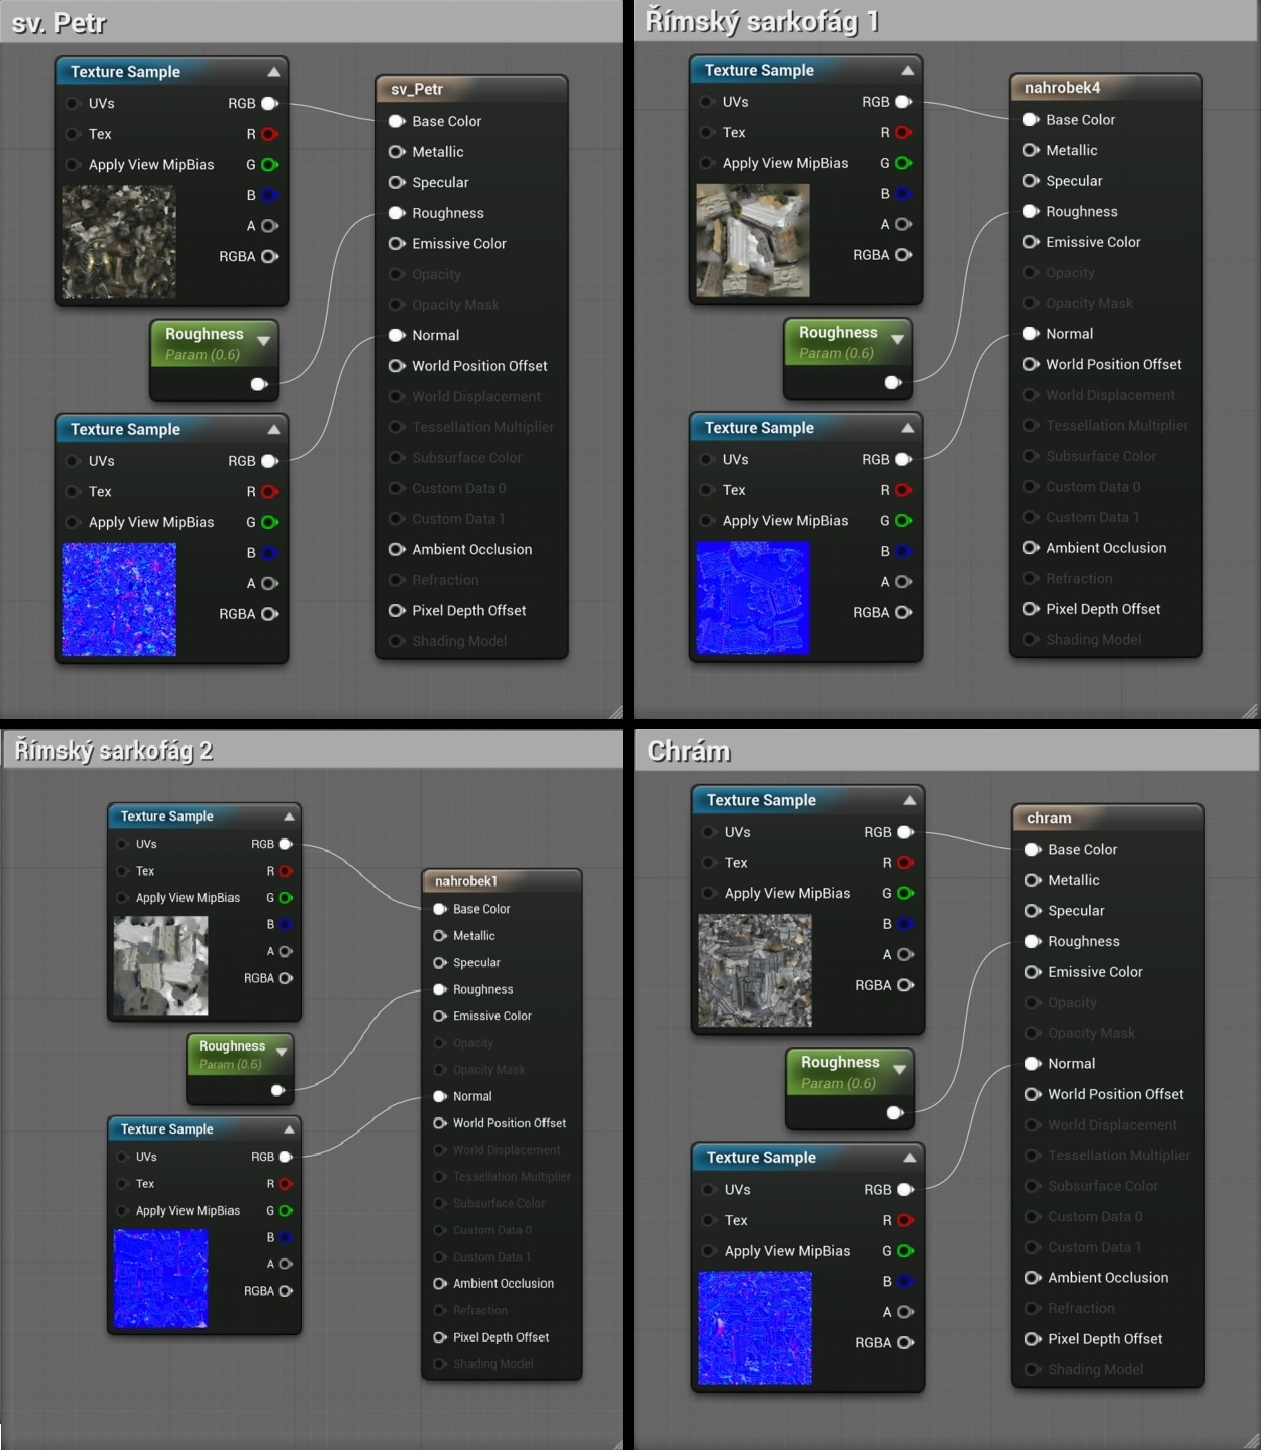
\includegraphics[width=12cm]{modely_materialy.jpg}
	\caption{Grafy nově vytvořených materiálů pro jednotlivé modely}
\end{figure}

\section{Umístění a nasvětlení modelů}
Umístění modelu do virtuálního světa lze provést jeho přetažením  ze složky projektu na požadované místo. Modely byly umístěni do vnitřních prostor budovy muzea a následně jim bylo nastaveno požadované měřítko. Exponáty byly umisťovány na expoziční boxy za účelem dosažení vysoké věrohodnosti virtuální výstavy. Po vhodném umístění a natočení objektů byly vytvořeny popisové tabule uvádějící názvy, měřítka a podrobné informace týkající se památek. \\
\\
Z důvodu špatných světelných podmínek uvnitř budovy bylo nutné vytvořit dodatečné osvětlení. Nástroj \textit{Place} v \textit{UE4} obsahuje záložku \textit{Lights}, ze které byla světla do prostoru uvnitř budovy umisťována. Umisťovaná světla byla typu \textit{Point Light} a byla nastavena jako statická.

\begin{figure}[h!]
	\centering
	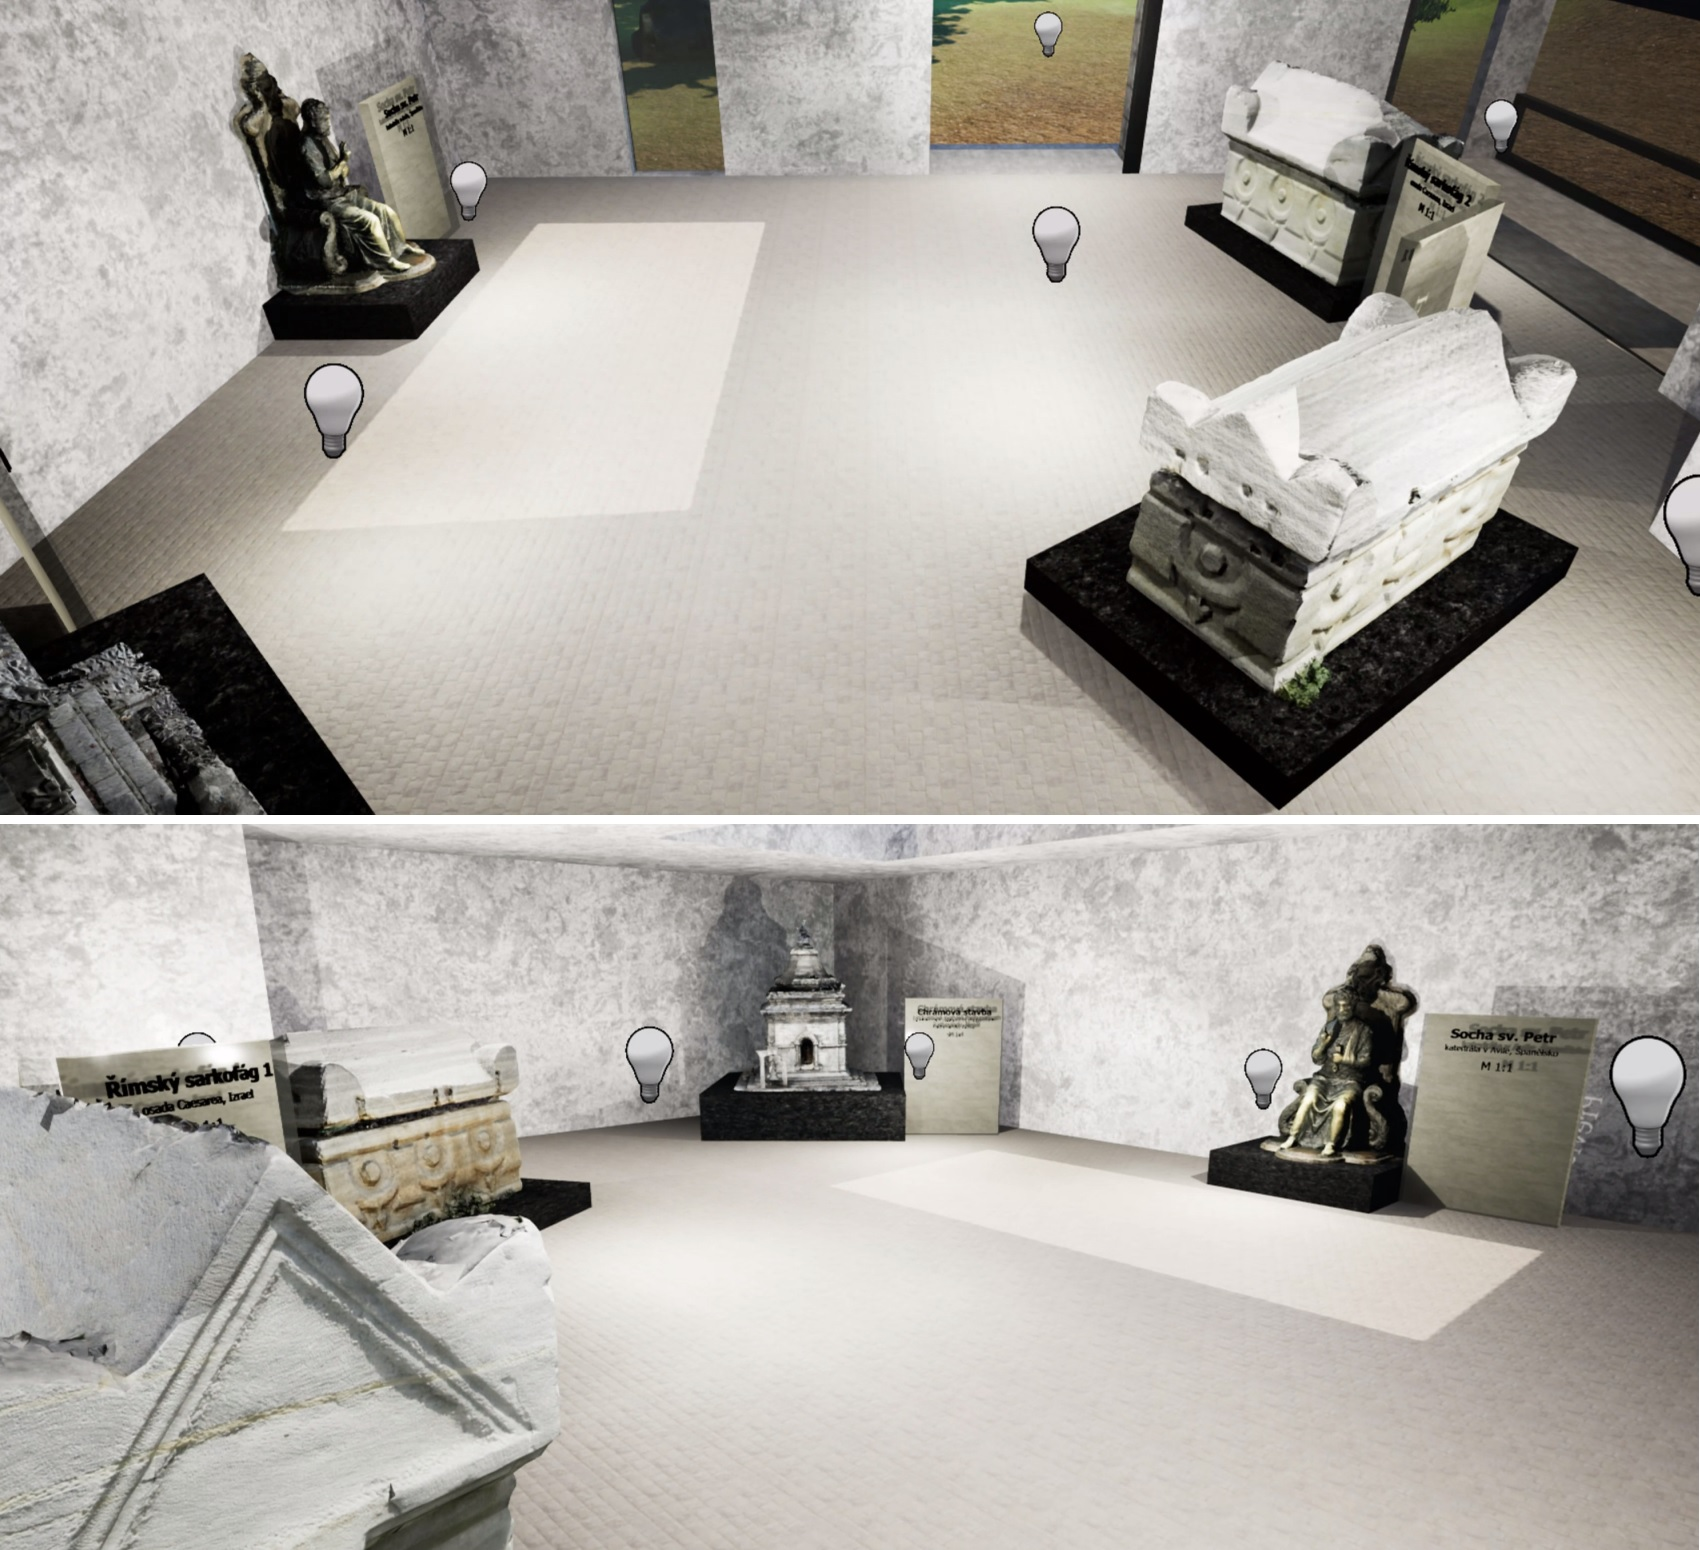
\includegraphics[width=16cm]{svetla.jpg}
	\caption{Rozmístění světel uvnitř virtuálního muzea}
\end{figure}

\chapter{Diskuze}
Hlavním cílem této práce bylo ukázat možnosti využití VR pro dokumentaci a vizualizaci památkových objektů. Pro účely vizualizace ve VR bylo vytvořeno virtuální muzeum, které obsahuje modely objektů zpracované fotogrammetrickou metodou IBMR.\\
\\
V současné době má zájem o historii mezi širokou veřejností značně rostoucí tendenci. Tuto skutečnost lze velmi dobře pozorovat i během aktuální situace, kdy světem hýbe pandemie COVID-19. Mnoho regionů, navštěvovaných masami lidí především pro své kulturní dědictví, je nyní téměř vylidněno. Způsoby, kterými mohou lidé během současné krize památky navštěvovat, jsou značně omezené. Omezení turismu v památkových oblastech má ale také světlé stránky. Historické relikvie, budovy, sochy atd. nejsou bezohlednými návštěvníky poškozovány. Umožnění přístupu k významným historickým objektům široké veřejnosti a zároveň omezení či vyloučení jejich poškození z důvodu neodborného zacházení jsou aktuální témata, kterým je věnována i tato práce. Jedním z možných řešení výše uvedeného problému jsou různé formy virtuálních muzeí. Ta jsou v současné době vyspělých virtuálních technologií snadno přístupná a zároveň vylučují možnost neodborného zacházení s exponáty. Další výhodou takového muzea je možnost alespoň částečné interakce uživatele s vystavovanými předměty. Hlavní nevýhoda využití VR v předešlých letech, která spočívala v nedostatečné kvalitě virtuálního zážitku pro účely vizualizace historických objektů, je díky prudkému rozvoji volně dostupného hardwaru i softwaru téměř potlačena. VR se v současné době jeví jako ideální nástroj pro zprostředkování zážitků ve formě virtuální výstavy.\\
\\
Kvalita virtuálního muzea přímo závisí na metodách sběru dat a použité technologii při tvorbě modelů. Pokud má mít vznikající virtuální muzeum edukační charakter a přínos pro širokou i odbornou veřejnost, musí exponáty v něm obsažené dosahovat určitých kvalit. Na základě výsledků této práce lze říci, že vhodnými prostředky pro dokumentaci a následnou vizualizaci památkových objektů ve VR jsou metody fotogrammetrie a pozemního laserového skenování.\\
\\
Součástí práce je rešerše literatury na témata týkající se VR, AR, metod sledování pohybu u VR i AR zařízení a využití fotogrammetrie a laserového skenování pro sběr dat. Jak je z rešerše zřejmé, virtuální muzea značně nabývají na významu především v horizontu posledních let. Převážná část práce je věnována VR. Na základě odborných zdrojů je zde VR úzce definována společně s vysvětlením čtyř klíčových pojmů: virtuální svět, ponoření, smyslová zpětná vazba a míra interaktivity. Následně je podrobně zmapován vývoj a historie v oblasti VR. Teoretická část práce dále obsahuje výčet a podrobný popis dostupného hardwaru pro zprostředkování zážitku ve formě VR, včetně moderních metod sledování pohybu používaných jednotlivými výrobci. Poslední sekce teoretické části popisuje fotogrammetrickou IBMR metodu zpracování dat. V této části je podrobně popsán vhodný postup pro sběr a zpracování dat touto metodou. Tato technologie byla použita také při tvorbě modelů v praktické části této práce. Její výhodou jsou minimální náklady na používanou techniku v porovnání s pozemním laserovým skenováním při dosažení výsledků obdobné kvality.\\
\\
Praktická část práce představuje a popisuje vhodný způsob sběru a následné vizualizace dat ve VR. Pro sběr dat je zde využito běžných fotoaparátů. Dokumentovány byly celkem čtyři objekty různých velikostí a složitostí geometrie. Na základě výsledků této práce lze říci, že běžně dostupné kompaktní fotoaparáty je možné, za předpokladu dobrých světelných podmínek, využít i pro dokumentaci a následnou vizualizaci historických objektů ve virtuálním světě. Ovšem například pro účely měřické by bylo nutné použití kvalitnějších zrcadlových fotoaparátů. Následné zpracování dat bylo provedeno IBMR technologií. Postup zpracování je v této práci podrobně popsán a vysvětlen. Problémová byla tvorba síťového modelu chrámu. Fotografie obsahující vnitřní prostory budovy nebyly automatizovaným procesem zorientovány. Jako řešení byla zvolena oddělená tvorba modelu vnitřní části chrámu, který byl ve finální fázi k hlavnímu modelu připojen prostřednictvím identických bodů. V souvislosti s nevhodným rozložením a obtížnou identifikací identických bodů, které bylo možné využít, má vnitřní část modelu spíše doplňující charakter. \\
\\
Velmi časově náročná byla část práce věnovaná tvorbě VR prostředí a přípravě vytvořených modelů pro následnou vizualizaci. Budova virtuálního muzea byla vytvořena v softwaru SketchUp. Dalším krokem bylo vytvoření nové virtuální krajiny, ve které se budova nachází. Tvorba probíhala v herním enginu \textit{UE4} z volně dostupných prostředků pro tyto účely. Výsledná virtuální krajina působí přirozeným dojmem, prvky v ní umístěné jsou cíleně nepravidelné a dynamické. Pro rozsáhlejší krajinu by bylo vhodnější zvolit nižší hustotu rozmístění flóry, na rozdíl od stavu v této práci, z důvodu vysokých nároků na výpočetní výkon zprostředkujícího zařízení. Vysoká hustota rozmístění, především stromů, má za účel uživatele obklopit a zaručit tak vysoké ponoření do virtuálního světa.\\
\\
Pro optimální vizualizaci modelů ve VR bylo nutné provést, z důvodu jejich značného datového objemu, retopologii a s tím následně spojenou tvorbu normálových map. Tento postup umožní snížení objemu načítaných a zobrazovaných dat s minimální ztrátou detailů objektu. Následně byl v \textit{UE4} vytvořen z textury a normálové mapy objektu nový materiál, který zajistil realistický vzhled povrchu exponátu.\\
\\
Výsledné virtuální muzeum společně s okolním prostředím je velmi realistické a přirozené. Zážitek uživatele bude jistě dostatečně pohlcující. U vystavených exponátů se podařilo dosáhnout požadované podrobnosti detailů s ohledem na účel vizualizace ve VR. Praktická část ukazuje vhodný a nízkonákladový způsob, jakým lze dokumentovat objekty pro účely památkové péče, společně s následnou vizualizací ve VR vhodnou pro širokou veřejnost, která uživatele přibližuje zážitku ve skutečném světě. Tvorba modelů a zpracování dat jsou díky modernímu softwaru značně zautomatizovány, ale bez odborných znalostí by nebylo možné dosáhnout požadované úrovně kvality. \\
\\
Potenciál propojení VR s metodami fotogrammetrie nebo laserového skenování je jistě stále nevyčerpaný. Možnost přemístit se během okamžiku přes kontinenty, ba dokonce planety, a studovat, objevovat či manipulovat s předměty na tisíce kilometrů vzdálených, často obtížně dostupných, bez možnosti jakéhokoliv poškození či újmy na zdraví uživatele, je směr, kterým se budou jistě mnohé vzdělávací i veřejné instituce vydávat. Například v současné době na mnoha školách praktikovaná distanční forma výuky by mohla být obohacena o společné exkurze prostřednictvím VR zážitku, kde by studenti historie mohli interagovat a pracovat s objekty z celého světa. Dalším, jistě v budoucnosti vhodným využitím kombinace fotogrammetrie a VR, je oblast vesmírného výzkumu. Dokumentace vesmírných těles a jevů z těsné blízkosti a následné vytvoření odpovídajícího virtuálního prostředí s vizualizací ve VR, by mohlo přenést uživatele do téměř identického prostoru, jako by ve vesmíru skutečně byl. To by zajisté usnadnilo výzkum a zároveň minimalizovalo finanční náročnost. 

\chapter{Závěr}
Cílem této práce bylo ukázat možnosti VR pro památkovou péči. Za tímto účelem bylo vytvořeno virtuální prostředí vhodné pro vizualizaci modelů skutečných historických objektů. Vizualizované modely v tomto prostředí byly vytvořeny fotogrammetrickou metodou prostřednictvím IBMR technologie z dat ve formě fotografií.\\
\\
Praktickou část této práce lze rozdělit na dva hlavní okruhy: tvorba virtuálního prostředí a tvorba modelů za účelem dokumentace a vizualizace historických objektů. Tvorba virtuálního prostředí probíhala v softwarech \textit{UE4} a \textit{SketchUp}. Byla vytvořena rozsáhlá virtuální krajina, do které byla umístěna budova muzea. Při tvorbě byl kladen důraz především na realističnost za účelem vysoké míry ponoření uživatele do VR. Krajinné prvky i flóra jsou nepravidelně rozmístěné a mají různé rozměry i tvary, některé elementy krajiny jsou dynamické a úspěšně tak simulují reálný svět. Pro některé elementy prostředí bylo nutné vytvoření nových materiálů. Tato tvorba byla realizována také v softwaru \textit{UE4}.\\
\\
Dokumentace historických objektů v této práci byla provedena běžně dostupnými fotoaparáty. Následné zpracování bylo realizováno ve specializovaném softwaru \textit{Agisoft Metashape}. Celkem byly vytvořeny 4 modely z téměř 250 fotografií. Modely následně prošly retopologií a byly jim vytvořeny normálové mapy textur.\\
\\
Závěrečné zpracování vizualizace, včetně tvorby materiálů a nasvícení objektů, ve VR bylo opět provedeno v softwaru \textit{UE4}. Výsledky této práce si lze prohlédnout prostřednictvím zařízení pro zprostředkování virtuální reality. Návštěvník virtuálního muzea má možnost se kochat okolním prostředím nebo se procházet uvnitř budovy, kde se nachází památkové objekty z různých částí světa. \\
\\
Prezentační video s názvem \textit{VR Museum}, obsahující náhled na část krajiny a exponáty v muzeu, je dostupné na serveru \textit{YouTube.com} [60].



\newpage

\renewcommand{\bibname}{Reference}
\begin{thebibliography}{9}

%Novák, J. 2013. Nové metody geomatiky. New horizons, vol.3, 23. ISBN 1234567, dostupný z: http://www.stavebníobzor.cz/2013/1/novak.pdf

\bibitem{1} Sherman, W., Craig, A. \textit{Understanding Virtual Reality : Interface, Application, and Design.} 1. vyd. Morgan Kaufman, 2002. ISBN: 9781558603530

\bibitem{2} University of Insubria \textit{Instant Field Aligned Meshes (SIGGRAPH ASIA 2015)}. \\YouTube [online]. 2015-9-25 [cit. 2020-5-17]. \\Dostupné z: \textit{https://www.youtube.com/watch?v=U6wtw6W4x3I}

\bibitem{3} The LATEX Project. [online]. [cit 2020-1-8]. Dostupné z: \textit{https://www.latex-project.org/}

\bibitem{4} The Virtual Reality Society. [online]. [cit. 2020-1-11]. \\Dostupné z: \textit{https://www.vrs.org.uk/}

\bibitem{5} Mazuryk, T., Gervautz, M. \textit{History, Applications, Technology and Future.} Institute of Computer Graphics, Vienna University of Technology, Austria.

\bibitem{6} Barnard, D. \textit{History of VR - Timeline of Events and Tech Development.} [online]. 2019-8-6 [cit. 2020-1-17]. Dostupné z: \textit{https://virtualspeech.com/blog/history-of-vr}

\bibitem{7} American Psychological Association. [online]. [cit. 2020-1-17]. \\Dostupné z: \textit{https://dictionary.apa.org/}

\bibitem{8} Sutherland, I.: \textit{The Ultimate Display.} Proceedings of the IFIP Congress, 1965. 506-508. [online]. [cit. 2020-1-17] \\Dostupné z: \textit{http://papers.cumincad.org/data/works/att/c58e.content.pdf}

\bibitem{9}  Jeremy Norman \textit{The DataGlove, a Hand Gesture Interface Device.} [online]. [cit. 2020-1-18]. Dostupné z: \textit{http://www.historyofinformation.com/detail.php?id=3626}

\bibitem{10} Sega Retro. \textit{VR-1.} [online]. [cit. 2020-1-18]. Dostupné z: \textit{https://segaretro.org/VR-1}

\bibitem{11} Filefacts.com. \textit{Virtools VR Pack.} [online]. 2015 [cit. 2020-1-18]. Dostupné z: \textit{http://www.filefacts.com/virtools-vr-pack-info}

\bibitem{12} Google. \textit{Používání funkce Street View v Mapách Google.} [online]. [cit. 2020-1-18]. Dostupné z: \textit{https://support.google.com/maps/}

\bibitem{13} IrisVR. [online]. [cit. 2020-1-19]. Dostupné z: \textit{https://irisvr.com/}

\bibitem{14} COMFOR. \textit{Jak výkonný počítač je potřeba pro virtuální realitu?} [online].\\ 2019-4-27 [cit. 2020-1-19]. Dostupné z: \textit{https://www.comfor.cz/blog/jak-vykonny-pocitac-je-potreba-pro-virtualni-reali}

\bibitem{15} rvdm88. \textit{How the Vive Lighthouse Works.} YouTube [online]. 2015-6-19 [cit. 2020-1-22]. Dostupné z: \textit{https://www.youtube.com/watch?v=oqPaaMR4kY4}

\bibitem{16} UVR Media. \textit{How VR Positional Tracking Systems Work.} [online]. 2019-4-29 [cit. 2020-1-22]. Dostupné z: \textit{https://uploadvr.com/how-vr-tracking-works/}

\bibitem{17} Nunez, M. \textit{HTC Vive Review: A Beautiful Machine With One Major Flaw.} Gizmondo. [online]. 2016-5-4 [cit. 2020-1-22]. Dostupné z: \textit{https://gizmodo.com/htc-vive-review-a-beautiful-machine-with-no-good-games-1768989238}

\bibitem{18} Nth Screen. \textit{Designing for VR: Beginners Guide for ID and IxD.} Barnes \& Noble.

\bibitem{19} Miller, P. \textit{HTC Vive guts reveal photodiodes and spinning lasers.} The Verge. [online]. 2016-4-26 [cit. 2020-1-22]. \\Dostupné z: \textit{https://www.theverge.com/2016/4/26/11509462/htc-vive-ifixit-teardown-photodiodes-spinny-lasers}

\bibitem{20} VIVE. [online]. [cit. 2020-1-29]. Dostupné z: \textit{https://www.vive.com/us/}

\bibitem{21} Najman, J. \textit{Aplikace SLAM algoritmů pro vozidlo s čtyřmu řízenými koly.} Brno, 2015. Diplomová práce. Vysoké učení technické v Brně, fakulta strojního inženýrství, ústav mechaniky těles, mechatroniky a biomechaniky.

\bibitem{22} Endicott, S. \textit{Oculus Quest: Everything you need to know!.} androidcentral. [online]. 2019-12-25 [cit. 2020-2-10]. Dostupné z: \textit{https://www.androidcentral.com/oculus-quest}

\bibitem{23} Oculus from facebook. [online]. [cit. 2020-2-10]. Dostupné z: \textit{https://www.oculus.com/}

\bibitem{24} PlayStation VR. [online]. [cit. 2020-2-14]. \\Dostupné z: \textit{https://www.playstation.com/cs-cz/explore/playstation-vr/}

\bibitem{25} Greenwald, W. \textit{Sony PlayStation VR Review.} PCMag. [online]. 2017-8-29 [cit. 2020-2-14]. Dostupné z: \textit{https://www.pcmag.com/reviews/sony-playstation-vr}

\bibitem{26}  Carbotte, K. \textit{Valve Index VR Headset and Controllers Review: A New Champion.} Tom's Hardware, Future US. [online]. 2020-2-25 [cit. 2020-2-14]. Dostupné z: \textit{https://www.tomshardware.com/reviews/valve-index-vr-headset-controllers,6205.html}

\bibitem{27} Valve Index. [online]. [cit. 2020-2-14]. Dostupné z: \textit{https://www.valvesoftware.com/cs/}

\bibitem{28} Pavelka, K. a kolektiv. \textit{Exaktní metody průzkumu památek s využitím geodetických a geofyzikálních metod.} 1. vyd. ČVUT, Praha, 2017. ISBN: 978-80-01-05260-0

\bibitem{29} Pavelka, K., Šedina, J., Matoušková, E., Faltýnová, M., Řezníček, J. \textit{Ověřená technologie nízkonákladové 3D fotogrammetrické dokumentace památkových objektů.} ČVUT, Praha, 2015 [cit. 2020-2-22]. Dostupné z: \textit{https://docplayer.cz/23740954-Overena-technologie-nizkonakladove-3d-fotogrammetricke-dokumentace-pamatkovych-objektu.html}

\bibitem{30} Campbell, D. \textit{6 Ways Virtual Reality Construction Technology Can Save You Money NOW}. Connect \& Construct. [online]. 2017-6-9 [cit. 2020-2-23]. Dostupné z: \textit{https://connect.bim360.autodesk.com/virtual-reality-construction-technology-saves-money}

\bibitem{31} Ma, D., Gausemeier, J., Fan, X., Grafe, M. \textit{Virtual Reality \& Augmented Reality in Industry.} Shanghai Jiao Tong University Press, Shanghai and Springer-Verlag Berlin Heidelberg, 2011.

\bibitem{32} Kysilka, M. \textit{VR kiosky od Amazonu představují budoucnost nakupování}. 6D HUB. [online]. 2018-8-2 [cit. 2020-2-23]. Dostupné z: \textit{https://www.6dhub.cz/virtualni-realita/virtualni-realita/vr-kiosky-od-amazonu-predstavuji-budoucnost-nakupovani/}

\bibitem{33} Carfagno, J. \textit{Top 4 Virtual Reality (VR) Breakthroughs in Medicine} docwirenews. [online]. 2019-12-1 [cit. 2020-2-27]. Dostupné z: \textit{https://www.docwirenews.com/docwire-pick/top-4-virtual-reality-vr-breakthroughs-in-medicine/}

\bibitem{34} Walczak, K., Cellary, W., White, M. \textit{Virtual Museum Exhibitions.} IEEE Computer, 39, 93–95. [online]. 2006 [cit. 2020-3-3]. \\Dostupné z: \textit{https://ieeexplore.ieee.org/abstract/document/1607962}

\bibitem{35} Jůva, V. \textit{Virtuální muzeum a nové možnosti
vzdělávání.} Mimoškolní edukační média. Pedagogická encyklopedie. Praha, Portál, 282–286, ISBN 978-80-7367-546-2. [online]. 2009 [cit. 2020-4-3]. Dostupné z: \textit{https://journals.muni.cz/pedor/article/view/1152/892}

\bibitem{36} SketchUp. Trimble. [online]. [cit. 2020-4-9]. Dostupné z: \textit{https://www.sketchup.com/}

\bibitem{37} Grand View Research \textit{Healthcare Augmented \& Virtual Reality Market Worth \$5.1 Billion By 2025.} [online]. 2017-6 [cit. 2020-4-12]. Dostupné z: \textit{https://www.grandview\\-research.com/press-release/global-augmented-reality-ar-virtual-reality-vr-in-healthcare-market}

\bibitem{38} Ribo, M., Pinz, A., Fuhrmann, A. L. \textit{A new optical tracking system for virtual and augmented reality applications}. IMTC 2001. Proceedings of the 18th IEEE Instrumentation and Measurement Technology Conference. Rediscovering Measurement in the Age of Informatics (Cat. No.01CH 37188), Budapest, 1932-1936. [online]. [cit. 2020-4-12].  Dostupné z: \textit{https://ieeexplore.ieee.org/abstract/document/929537}

\bibitem{39} LaValle, S. M., Yershova, A., Katsev, M., Antonov, M. \textit{Head Tracking for the Oculus Rift}, 2014 IEEE International Conference on Robotics and Automation (ICRA), Hong Kong, 187-194. 2014 [cit. 2020-4-12].  \\Dostupné z: \textit{https://ieeexplore.ieee.org/abstract/document/6906608}

\bibitem{40} Jašek, P. \textit{Zvyšovaní přesnosti dat 3D skenování pro geodetický monitoring.} Praha, 2018. Disertační práce. ČVUT, fakulta stavební,katedra speciální geodézie.

\bibitem{41} Bethany \textit{Everything You Need To Know About SketchUp} Scan2CAD. [online]. 2018-3-12 [cit. 2020-5-2]. Dostupné z: \textit{https://www.scan2cad.com/cad/everything-about-sketchup}

\bibitem{42} Unreal Engine. [online]. [cit. 2020-5-2]. Dostupné z: \textit{https://www.unrealengine.com/en-US/}

\bibitem{43} Unreal Engine 4 Documentation. Unreal Engine. [online]. [cit. 2020-5-3]. Dostupné z: \textit{https://docs.unrealengine.com/en-US/index.html}

\bibitem{44} FotoŠkoda \textit{RICOH G700SE}. [online]. [cit. 2020-5-7]. \\Dostupné z: \textit{https://www.fotoskoda.cz/ricoh-g700se/}

\bibitem{45} G4D \textit{Agisoft Metashape}. [online]. [cit. 2020-5-7]. Dostupné z: \textit{https://www.metashape.cz/}

\bibitem{46} Agisoft LLC \textit{Agisoft Metashape User Manual
Professional Edition.} [online]. [cit. 2020-5-7]. Dostupné z: \textit{https://www.agisoft.com/pdf/metashape-pro\textunderscore 1\textunderscore 5\textunderscore en.pdf}

\bibitem{47} ETH Zurich \textit{Instant Field-Aligned Meshes}. Intertactive geometry lab. [online]. [cit. 2020-5-9]. Dostupné z: \textit{https://igl.ethz.ch/projects/instant-meshes/}

\bibitem{48}Muñoz-Saavedra, L., Miró-Amarante, L., Domínguez-Morales, M. \textit{Augmented and Virtual Reality Evolution and Future Tendency} Applied Sciences 10.1: 322. [online].2020 [cit. 2020-5-9]. Dostupné z: \textit{https://www.mdpi.com/2076-3417/10/1/322}

\bibitem{49} LaValle, M. S. \textit{Virtual Reality}. Cambridge University Press. [online]. 2015 [cit. 2020-5-11] Dostupné z: \textit{http://lavalle.pl/vr/}

\bibitem{50} Yastikli, N. \textit{Documentation of cultural heritage using digital photogrammetry and laser scanning.} Journal of Cultural Heritage, 423-427. [online]. 2007 [cit. 2020-5-11] Dostupné z: \textit{https://www.sciencedirect.com/science/article/abs/pii/S1296207407001082}

\bibitem{51} Grussenmeyer, P., Landes, T., Voegtle, T., Ringle, K. \textit{Comparison methods of terrestrial laser scanning, photogrammetry and tacheometry data for recording of cultural heritage buildings.} International Archives of Photogrammetry, Remote Sensing and Spatial Information Sciences, 213-218.

\bibitem{52} Furht, B.: \textit{Handbook of Augmented Reality.} Springer Science \& Business Media. 2011 [cit. 2020-5-10]

\bibitem{53} Carmigniani, J., Furht, B., Anisetti, M., Ceravolo, P., Damiani, E., Ivkovic, M.: \textit{Augmented reality technologies, systems and applications}. Multimedia tools and applications, 341-377. [online]. 2011 [cit. 2020-5-12]. Dostupné z: \textit{https://link.springer.com/art-icle/10.1007\%2Fs11042-010-0660-6}

\bibitem{54} Jung, T., Dieck, M. C., Lee, H., Chung, N. \textit{Effects of Virtual Reality and Augmented Reality on Visitor Experiences in Museum}. Information and communication technologies in tourism, 621-635. [online]. 2016 [cit. 2020-5-12]. Dostupné z: \textit{https://link.springer.com/chapter/10.1007/978-3-319-28231-2\textunderscore 45}

\bibitem{55} Denham, D.\textit{ What is UV Mapping \& Unwrapping?}. Concept Art Empire. [online]. [cit. 2020-5-13]. Dostupné z: \textit{https://conceptartempire.com/uv-mapping-unwrapping/}

\bibitem{56} VR Education. \textit{Virtuální realita – historie a současnost.} [online]. [cit. 2020-5-17]. Dostupné z: \textit{https://vreducation.cz/virtualni-realita-historie-a-soucasnost/}

\bibitem{57} Halata, O. \textit{HTC Vive má potvrzenou cenovku.} Android market. [online]. 2016-2-22 [cit. 2020-5-17]. Dostupné z: \textit{https://androidmarket.cz/ruzne/htc-vive-ma-potvrzenou-cenovku/}

\bibitem{58} Polygon Academy \textit{UNREAL ENGINE 4 LIGHTING TUTORIAL (UE4) - FREE DOWNLOAD LINK INCLUDED}. YouTube [online]. 2015-3-21 [cit. 2020-5-17]. Dostupné z: \textit{https://www.youtube.com/watch?v=\_bqpw5sOwr4}

\bibitem{59} Polygon Academy \textit{UE4 Lighting Presets 3 Pack}. Gumroad [online]. [cit. 2020-5-17]. Dostupné z: \textit{https://gumroad.com/l/ue4light}

\bibitem{60} Robin Pflug \textit{VR Museum}. YouTube [online]. 2020-23-5. [cit. 2020-23-5]. Dostupné z: \textit{https://youtu.be/7Yv9p6NI5Lk}

\newpage
\chapter{Přílohy}
\section{Příloha A - Reporty}
Výstupy ve formě reportů z tvorby \textit{high-poly} modelů v softwaru \textit{Agisoft Metashape}.

\begin{enumerate}

\item \textit{Report\textunderscore Sv\textunderscore Petr.pdf} - Report z tvorby modelu sochy sv. Petra.

\item \textit{Report\textunderscore Sarkofág\textunderscore 1.pdf} - Report z tvorby modelu Římského sarkofágu 1.

\item \textit{Report\textunderscore Sarkofág\textunderscore 2.pdf} - Report z tvorby modelu Římského sarkofágu 2.

\item \textit{Report\textunderscore Chrám\textunderscore vnitřní\textunderscore část.pdf} - Report z tvorby modelu vnitřní části chrámu.

\item \textit{Report\textunderscore Chrám\textunderscore vnější\textunderscore část.pdf} - Report z tvorby modelu vnější části chrámu.

\item \textit{Report\textunderscore Chrám.pdf} - Report z tvorby kompletního modelu chrámu.

\end{enumerate}


\section{Příloha B - Obsah přiloženého USB flash drivu}
USB flash drive obsahuje kompletní projekt Virtuálního muzea.\\
Obsahem je dále soubor readme.txt, ve kterém se nachází popis obsahu USB flash drivu, složka LaTex obsahující zdrojovou formu práce a složka text obsahující text práce ve formátu PDF.

\end{thebibliography}
\end{document}